\documentclass[twoside]{book}

% Packages required by doxygen
\usepackage{fixltx2e}
\usepackage{calc}
\usepackage{doxygen}
\usepackage[export]{adjustbox} % also loads graphicx
\usepackage{graphicx}
\usepackage[utf8]{inputenc}
\usepackage{makeidx}
\usepackage{multicol}
\usepackage{multirow}
\PassOptionsToPackage{warn}{textcomp}
\usepackage{textcomp}
\usepackage[nointegrals]{wasysym}
\usepackage[table]{xcolor}

% Font selection
\usepackage[T1]{fontenc}
\usepackage[scaled=.90]{helvet}
\usepackage{courier}
\usepackage{amssymb}
\usepackage{sectsty}
\renewcommand{\familydefault}{\sfdefault}
\allsectionsfont{%
  \fontseries{bc}\selectfont%
  \color{darkgray}%
}
\renewcommand{\DoxyLabelFont}{%
  \fontseries{bc}\selectfont%
  \color{darkgray}%
}
\newcommand{\+}{\discretionary{\mbox{\scriptsize$\hookleftarrow$}}{}{}}

% Page & text layout
\usepackage{geometry}
\geometry{%
  a4paper,%
  top=2.5cm,%
  bottom=2.5cm,%
  left=2.5cm,%
  right=2.5cm%
}
\tolerance=750
\hfuzz=15pt
\hbadness=750
\setlength{\emergencystretch}{15pt}
\setlength{\parindent}{0cm}
\setlength{\parskip}{3ex plus 2ex minus 2ex}
\makeatletter
\renewcommand{\paragraph}{%
  \@startsection{paragraph}{4}{0ex}{-1.0ex}{1.0ex}{%
    \normalfont\normalsize\bfseries\SS@parafont%
  }%
}
\renewcommand{\subparagraph}{%
  \@startsection{subparagraph}{5}{0ex}{-1.0ex}{1.0ex}{%
    \normalfont\normalsize\bfseries\SS@subparafont%
  }%
}
\makeatother

% Headers & footers
\usepackage{fancyhdr}
\pagestyle{fancyplain}
\fancyhead[LE]{\fancyplain{}{\bfseries\thepage}}
\fancyhead[CE]{\fancyplain{}{}}
\fancyhead[RE]{\fancyplain{}{\bfseries\leftmark}}
\fancyhead[LO]{\fancyplain{}{\bfseries\rightmark}}
\fancyhead[CO]{\fancyplain{}{}}
\fancyhead[RO]{\fancyplain{}{\bfseries\thepage}}
\fancyfoot[LE]{\fancyplain{}{}}
\fancyfoot[CE]{\fancyplain{}{}}
\fancyfoot[RE]{\fancyplain{}{\bfseries\scriptsize Generated by Doxygen }}
\fancyfoot[LO]{\fancyplain{}{\bfseries\scriptsize Generated by Doxygen }}
\fancyfoot[CO]{\fancyplain{}{}}
\fancyfoot[RO]{\fancyplain{}{}}
\renewcommand{\footrulewidth}{0.4pt}
\renewcommand{\chaptermark}[1]{%
  \markboth{#1}{}%
}
\renewcommand{\sectionmark}[1]{%
  \markright{\thesection\ #1}%
}

% Indices & bibliography
\usepackage{natbib}
\usepackage[titles]{tocloft}
\setcounter{tocdepth}{3}
\setcounter{secnumdepth}{5}
\makeindex

% Hyperlinks (required, but should be loaded last)
\usepackage{ifpdf}
\ifpdf
  \usepackage[pdftex,pagebackref=true]{hyperref}
\else
  \usepackage[ps2pdf,pagebackref=true]{hyperref}
\fi
\hypersetup{%
  colorlinks=true,%
  linkcolor=blue,%
  citecolor=blue,%
  unicode%
}

% Custom commands
\newcommand{\clearemptydoublepage}{%
  \newpage{\pagestyle{empty}\cleardoublepage}%
}

\usepackage{caption}
\captionsetup{labelsep=space,justification=centering,font={bf},singlelinecheck=off,skip=4pt,position=top}

%===== C O N T E N T S =====

\begin{document}

% Titlepage & ToC
\hypersetup{pageanchor=false,
             bookmarksnumbered=true,
             pdfencoding=unicode
            }
\pagenumbering{roman}
\begin{titlepage}
\vspace*{7cm}
\begin{center}%
{\Large qecc \\[1ex]\large 0.\+8 }\\
\vspace*{1cm}
{\large Generated by Doxygen 1.8.11}\\
\end{center}
\end{titlepage}
\clearemptydoublepage
\tableofcontents
\clearemptydoublepage
\pagenumbering{arabic}
\hypersetup{pageanchor=true}

%--- Begin generated contents ---
\chapter{qecc}
\label{md__home_attila_src_qecc-netbeans_qecc_README}
\hypertarget{md__home_attila_src_qecc-netbeans_qecc_README}{}
Quantum error correcting code simulator 
\chapter{Hierarchical Index}
\section{Class Hierarchy}
This inheritance list is sorted roughly, but not completely, alphabetically\+:\begin{DoxyCompactList}
\item \contentsline{section}{Channel}{\pageref{class_channel}}{}
\item \contentsline{section}{Code}{\pageref{class_code}}{}
\begin{DoxyCompactList}
\item \contentsline{section}{Aad4}{\pageref{class_aad4}}{}
\item \contentsline{section}{Bit\+Flip}{\pageref{class_bit_flip}}{}
\item \contentsline{section}{Code5}{\pageref{class_code5}}{}
\item \contentsline{section}{None}{\pageref{class_none}}{}
\item \contentsline{section}{Shor}{\pageref{class_shor}}{}
\item \contentsline{section}{Steane}{\pageref{class_steane}}{}
\end{DoxyCompactList}
\item \contentsline{section}{Error}{\pageref{class_error}}{}
\item \contentsline{section}{Node}{\pageref{class_node}}{}
\item \contentsline{section}{Runable}{\pageref{class_runable}}{}
\begin{DoxyCompactList}
\item \contentsline{section}{Network}{\pageref{class_network}}{}
\item \contentsline{section}{Single}{\pageref{class_single}}{}
\item \contentsline{section}{Test}{\pageref{class_test}}{}
\end{DoxyCompactList}
\item \contentsline{section}{Runner}{\pageref{class_runner}}{}
\end{DoxyCompactList}

\chapter{Class Index}
\section{Class List}
Here are the classes, structs, unions and interfaces with brief descriptions\+:\begin{DoxyCompactList}
\item\contentsline{section}{\hyperlink{class_aad4}{Aad4} }{\pageref{class_aad4}}{}
\item\contentsline{section}{\hyperlink{class_bit_flip}{Bit\+Flip} }{\pageref{class_bit_flip}}{}
\item\contentsline{section}{\hyperlink{class_channel}{Channel} }{\pageref{class_channel}}{}
\item\contentsline{section}{\hyperlink{class_code}{Code} }{\pageref{class_code}}{}
\item\contentsline{section}{\hyperlink{class_code5}{Code5} }{\pageref{class_code5}}{}
\item\contentsline{section}{\hyperlink{class_error}{Error} }{\pageref{class_error}}{}
\item\contentsline{section}{\hyperlink{class_network}{Network} }{\pageref{class_network}}{}
\item\contentsline{section}{\hyperlink{class_node}{Node} }{\pageref{class_node}}{}
\item\contentsline{section}{\hyperlink{class_none}{None} }{\pageref{class_none}}{}
\item\contentsline{section}{\hyperlink{class_runable}{Runable} }{\pageref{class_runable}}{}
\item\contentsline{section}{\hyperlink{class_runner}{Runner} }{\pageref{class_runner}}{}
\item\contentsline{section}{\hyperlink{class_shor}{Shor} }{\pageref{class_shor}}{}
\item\contentsline{section}{\hyperlink{class_single}{Single} }{\pageref{class_single}}{}
\item\contentsline{section}{\hyperlink{class_steane}{Steane} }{\pageref{class_steane}}{}
\item\contentsline{section}{\hyperlink{class_test}{Test} }{\pageref{class_test}}{}
\end{DoxyCompactList}

\chapter{File Index}
\section{File List}
Here is a list of all files with brief descriptions\+:\begin{DoxyCompactList}
\item\contentsline{section}{/home/attila/src/qecc-\/netbeans/qecc/\hyperlink{_8dep_8inc}{.\+dep.\+inc} }{\pageref{_8dep_8inc}}{}
\item\contentsline{section}{/home/attila/src/qecc-\/netbeans/qecc/\hyperlink{_aad4_8cpp}{Aad4.\+cpp} }{\pageref{_aad4_8cpp}}{}
\item\contentsline{section}{/home/attila/src/qecc-\/netbeans/qecc/\hyperlink{_aad4_8h}{Aad4.\+h} }{\pageref{_aad4_8h}}{}
\item\contentsline{section}{/home/attila/src/qecc-\/netbeans/qecc/\hyperlink{_bit_flip_8cpp}{Bit\+Flip.\+cpp} }{\pageref{_bit_flip_8cpp}}{}
\item\contentsline{section}{/home/attila/src/qecc-\/netbeans/qecc/\hyperlink{_bit_flip_8h}{Bit\+Flip.\+h} }{\pageref{_bit_flip_8h}}{}
\item\contentsline{section}{/home/attila/src/qecc-\/netbeans/qecc/\hyperlink{_channel_8cpp}{Channel.\+cpp} }{\pageref{_channel_8cpp}}{}
\item\contentsline{section}{/home/attila/src/qecc-\/netbeans/qecc/\hyperlink{_channel_8h}{Channel.\+h} }{\pageref{_channel_8h}}{}
\item\contentsline{section}{/home/attila/src/qecc-\/netbeans/qecc/\hyperlink{_code_8cpp}{Code.\+cpp} }{\pageref{_code_8cpp}}{}
\item\contentsline{section}{/home/attila/src/qecc-\/netbeans/qecc/\hyperlink{_code_8h}{Code.\+h} }{\pageref{_code_8h}}{}
\item\contentsline{section}{/home/attila/src/qecc-\/netbeans/qecc/\hyperlink{_code5_8cpp}{Code5.\+cpp} }{\pageref{_code5_8cpp}}{}
\item\contentsline{section}{/home/attila/src/qecc-\/netbeans/qecc/\hyperlink{_code5_8h}{Code5.\+h} }{\pageref{_code5_8h}}{}
\item\contentsline{section}{/home/attila/src/qecc-\/netbeans/qecc/\hyperlink{_error_8cpp}{Error.\+cpp} }{\pageref{_error_8cpp}}{}
\item\contentsline{section}{/home/attila/src/qecc-\/netbeans/qecc/\hyperlink{_error_8h}{Error.\+h} }{\pageref{_error_8h}}{}
\item\contentsline{section}{/home/attila/src/qecc-\/netbeans/qecc/\hyperlink{_network_8cpp}{Network.\+cpp} }{\pageref{_network_8cpp}}{}
\item\contentsline{section}{/home/attila/src/qecc-\/netbeans/qecc/\hyperlink{_network_8h}{Network.\+h} }{\pageref{_network_8h}}{}
\item\contentsline{section}{/home/attila/src/qecc-\/netbeans/qecc/\hyperlink{_node_8cpp}{Node.\+cpp} }{\pageref{_node_8cpp}}{}
\item\contentsline{section}{/home/attila/src/qecc-\/netbeans/qecc/\hyperlink{_node_8h}{Node.\+h} }{\pageref{_node_8h}}{}
\item\contentsline{section}{/home/attila/src/qecc-\/netbeans/qecc/\hyperlink{_none_8cpp}{None.\+cpp} }{\pageref{_none_8cpp}}{}
\item\contentsline{section}{/home/attila/src/qecc-\/netbeans/qecc/\hyperlink{_none_8h}{None.\+h} }{\pageref{_none_8h}}{}
\item\contentsline{section}{/home/attila/src/qecc-\/netbeans/qecc/\hyperlink{qecc_8cpp}{qecc.\+cpp} }{\pageref{qecc_8cpp}}{}
\item\contentsline{section}{/home/attila/src/qecc-\/netbeans/qecc/\hyperlink{_runable_8cpp}{Runable.\+cpp} }{\pageref{_runable_8cpp}}{}
\item\contentsline{section}{/home/attila/src/qecc-\/netbeans/qecc/\hyperlink{_runable_8h}{Runable.\+h} }{\pageref{_runable_8h}}{}
\item\contentsline{section}{/home/attila/src/qecc-\/netbeans/qecc/\hyperlink{_runner_8cpp}{Runner.\+cpp} }{\pageref{_runner_8cpp}}{}
\item\contentsline{section}{/home/attila/src/qecc-\/netbeans/qecc/\hyperlink{_runner_8h}{Runner.\+h} }{\pageref{_runner_8h}}{}
\item\contentsline{section}{/home/attila/src/qecc-\/netbeans/qecc/\hyperlink{_shor_8cpp}{Shor.\+cpp} }{\pageref{_shor_8cpp}}{}
\item\contentsline{section}{/home/attila/src/qecc-\/netbeans/qecc/\hyperlink{_shor_8h}{Shor.\+h} }{\pageref{_shor_8h}}{}
\item\contentsline{section}{/home/attila/src/qecc-\/netbeans/qecc/\hyperlink{_single_8cpp}{Single.\+cpp} }{\pageref{_single_8cpp}}{}
\item\contentsline{section}{/home/attila/src/qecc-\/netbeans/qecc/\hyperlink{_single_8h}{Single.\+h} }{\pageref{_single_8h}}{}
\item\contentsline{section}{/home/attila/src/qecc-\/netbeans/qecc/\hyperlink{_steane_8cpp}{Steane.\+cpp} }{\pageref{_steane_8cpp}}{}
\item\contentsline{section}{/home/attila/src/qecc-\/netbeans/qecc/\hyperlink{_steane_8h}{Steane.\+h} }{\pageref{_steane_8h}}{}
\item\contentsline{section}{/home/attila/src/qecc-\/netbeans/qecc/\hyperlink{_test_8cpp}{Test.\+cpp} }{\pageref{_test_8cpp}}{}
\item\contentsline{section}{/home/attila/src/qecc-\/netbeans/qecc/\hyperlink{_test_8h}{Test.\+h} }{\pageref{_test_8h}}{}
\end{DoxyCompactList}

\chapter{Class Documentation}
\hypertarget{class_aad4}{}\section{Aad4 Class Reference}
\label{class_aad4}\index{Aad4@{Aad4}}


{\ttfamily \#include $<$Aad4.\+h$>$}



Inheritance diagram for Aad4\+:
\nopagebreak
\begin{figure}[H]
\begin{center}
\leavevmode
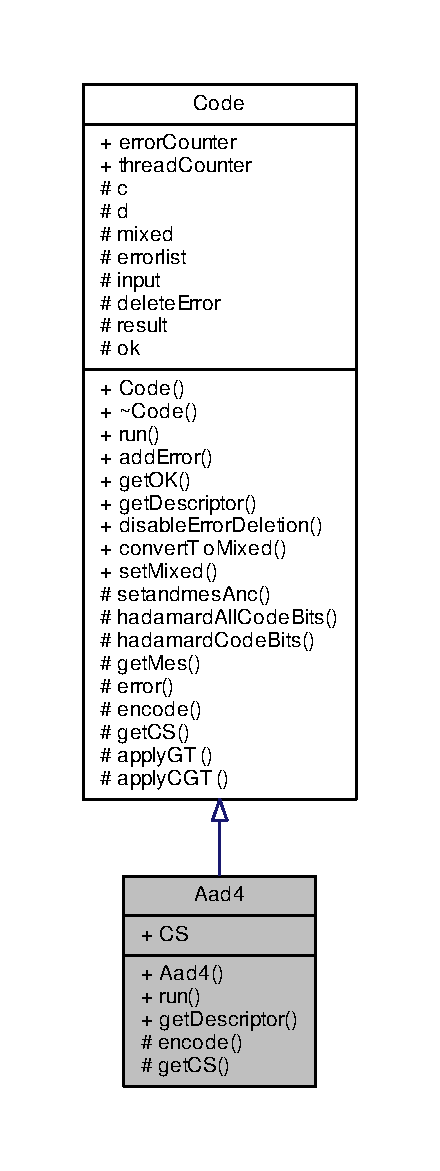
\includegraphics[height=550pt]{class_aad4__inherit__graph}
\end{center}
\end{figure}
\subsection*{Public Member Functions}
\begin{DoxyCompactItemize}
\item 
\hyperlink{class_aad4_af5a8655a7236239eeaddd65fb04bbf98}{Aad4} (bool b)
\item 
bool \hyperlink{class_aad4_a95f5ec483584c48bde0fd96d4d347c34}{run} () override
\item 
std\+::string \hyperlink{class_aad4_ad697e56ab152cd1228bd26f73451ec42}{get\+Descriptor} () override
\end{DoxyCompactItemize}
\subsection*{Static Public Attributes}
\begin{DoxyCompactItemize}
\item 
static const unsigned \hyperlink{class_aad4_a342120f0f5c7fe2240ad1de4bbda3a1b}{CS} = 4
\end{DoxyCompactItemize}
\subsection*{Protected Member Functions}
\begin{DoxyCompactItemize}
\item 
void \hyperlink{class_aad4_ad3febfa430563be08f78c3b7e8517ff6}{encode} (bool b) override
\item 
void \hyperlink{class_aad4_a48a811e7fc947a8da71fee4adecebff7}{decode} ()
\item 
unsigned \hyperlink{class_aad4_af4cb779e50399fcdca7a2f62282b7e78}{get\+CS} () override
\item 
bool \hyperlink{class_aad4_a6346f183da2c906f57113cb1c061822a}{no\+Error\+Op} ()
\item 
bool \hyperlink{class_aad4_ad36e1bd0550df1266efc3987207b4686}{error\+Op} (bool $\ast$f)
\item 
bool $\ast$ \hyperlink{class_aad4_ab0e6b87b58a9b73f6bfeb4eeba7bf1d4}{setandmes2\+Anc} ()
\end{DoxyCompactItemize}
\subsection*{Additional Inherited Members}


\subsection{Constructor \& Destructor Documentation}
\index{Aad4@{Aad4}!Aad4@{Aad4}}
\index{Aad4@{Aad4}!Aad4@{Aad4}}
\subsubsection[{\texorpdfstring{Aad4(bool b)}{Aad4(bool b)}}]{\setlength{\rightskip}{0pt plus 5cm}Aad4\+::\+Aad4 (
\begin{DoxyParamCaption}
\item[{bool}]{b}
\end{DoxyParamCaption}
)\hspace{0.3cm}{\ttfamily [inline]}}\hypertarget{class_aad4_af5a8655a7236239eeaddd65fb04bbf98}{}\label{class_aad4_af5a8655a7236239eeaddd65fb04bbf98}


\subsection{Member Function Documentation}
\index{Aad4@{Aad4}!decode@{decode}}
\index{decode@{decode}!Aad4@{Aad4}}
\subsubsection[{\texorpdfstring{decode()}{decode()}}]{\setlength{\rightskip}{0pt plus 5cm}void Aad4\+::decode (
\begin{DoxyParamCaption}
{}
\end{DoxyParamCaption}
)\hspace{0.3cm}{\ttfamily [protected]}}\hypertarget{class_aad4_a48a811e7fc947a8da71fee4adecebff7}{}\label{class_aad4_a48a811e7fc947a8da71fee4adecebff7}
\index{Aad4@{Aad4}!encode@{encode}}
\index{encode@{encode}!Aad4@{Aad4}}
\subsubsection[{\texorpdfstring{encode(bool b) override}{encode(bool b) override}}]{\setlength{\rightskip}{0pt plus 5cm}void Aad4\+::encode (
\begin{DoxyParamCaption}
\item[{bool}]{b}
\end{DoxyParamCaption}
)\hspace{0.3cm}{\ttfamily [override]}, {\ttfamily [protected]}, {\ttfamily [virtual]}}\hypertarget{class_aad4_ad3febfa430563be08f78c3b7e8517ff6}{}\label{class_aad4_ad3febfa430563be08f78c3b7e8517ff6}
Encode input bit 
\begin{DoxyParams}{Parameters}
{\em b} & Classical input converted to $\vert$0$>$ or $\vert$1$>$ \\
\hline
\end{DoxyParams}


Implements \hyperlink{class_code_a5f90b0f96002c9b999d8ed7bab319906}{Code}.

\index{Aad4@{Aad4}!error\+Op@{error\+Op}}
\index{error\+Op@{error\+Op}!Aad4@{Aad4}}
\subsubsection[{\texorpdfstring{error\+Op(bool $\ast$f)}{errorOp(bool *f)}}]{\setlength{\rightskip}{0pt plus 5cm}bool Aad4\+::error\+Op (
\begin{DoxyParamCaption}
\item[{bool $\ast$}]{f}
\end{DoxyParamCaption}
)\hspace{0.3cm}{\ttfamily [protected]}}\hypertarget{class_aad4_ad36e1bd0550df1266efc3987207b4686}{}\label{class_aad4_ad36e1bd0550df1266efc3987207b4686}
\index{Aad4@{Aad4}!get\+CS@{get\+CS}}
\index{get\+CS@{get\+CS}!Aad4@{Aad4}}
\subsubsection[{\texorpdfstring{get\+C\+S() override}{getCS() override}}]{\setlength{\rightskip}{0pt plus 5cm}unsigned Aad4\+::get\+CS (
\begin{DoxyParamCaption}
{}
\end{DoxyParamCaption}
)\hspace{0.3cm}{\ttfamily [inline]}, {\ttfamily [override]}, {\ttfamily [protected]}, {\ttfamily [virtual]}}\hypertarget{class_aad4_af4cb779e50399fcdca7a2f62282b7e78}{}\label{class_aad4_af4cb779e50399fcdca7a2f62282b7e78}
Return code size of a child \begin{DoxyReturn}{Returns}
code size 
\end{DoxyReturn}


Implements \hyperlink{class_code_a34f52b25d78aeaec3c1fd381f025ad00}{Code}.

\index{Aad4@{Aad4}!get\+Descriptor@{get\+Descriptor}}
\index{get\+Descriptor@{get\+Descriptor}!Aad4@{Aad4}}
\subsubsection[{\texorpdfstring{get\+Descriptor() override}{getDescriptor() override}}]{\setlength{\rightskip}{0pt plus 5cm}std\+::string Aad4\+::get\+Descriptor (
\begin{DoxyParamCaption}
{}
\end{DoxyParamCaption}
)\hspace{0.3cm}{\ttfamily [override]}, {\ttfamily [virtual]}}\hypertarget{class_aad4_ad697e56ab152cd1228bd26f73451ec42}{}\label{class_aad4_ad697e56ab152cd1228bd26f73451ec42}
Log of run ~\newline
 To be defined in child class ~\newline
 Contains code type, input, output, ancilla bit measurements ~\newline
 Format\+:~\newline
 {\itshape C\+O\+D\+E\+T\+Y\+PE ancillas input-\/$>$result O\+K/\+E\+R\+R\+OR} \begin{DoxyReturn}{Returns}
log string 
\end{DoxyReturn}


Implements \hyperlink{class_code_a60db2f615a7cff76e3ece1c486b2fd16}{Code}.

\index{Aad4@{Aad4}!no\+Error\+Op@{no\+Error\+Op}}
\index{no\+Error\+Op@{no\+Error\+Op}!Aad4@{Aad4}}
\subsubsection[{\texorpdfstring{no\+Error\+Op()}{noErrorOp()}}]{\setlength{\rightskip}{0pt plus 5cm}bool Aad4\+::no\+Error\+Op (
\begin{DoxyParamCaption}
{}
\end{DoxyParamCaption}
)\hspace{0.3cm}{\ttfamily [protected]}}\hypertarget{class_aad4_a6346f183da2c906f57113cb1c061822a}{}\label{class_aad4_a6346f183da2c906f57113cb1c061822a}
\index{Aad4@{Aad4}!run@{run}}
\index{run@{run}!Aad4@{Aad4}}
\subsubsection[{\texorpdfstring{run() override}{run() override}}]{\setlength{\rightskip}{0pt plus 5cm}bool Aad4\+::run (
\begin{DoxyParamCaption}
{}
\end{DoxyParamCaption}
)\hspace{0.3cm}{\ttfamily [override]}, {\ttfamily [virtual]}}\hypertarget{class_aad4_a95f5ec483584c48bde0fd96d4d347c34}{}\label{class_aad4_a95f5ec483584c48bde0fd96d4d347c34}
Function to simulate the transmission and get the result. To be defined in child classes. \begin{DoxyReturn}{Returns}
Measured bit at Bob 
\end{DoxyReturn}


Implements \hyperlink{class_code_a5621bbd050948ba1e41f69f451a05990}{Code}.

\index{Aad4@{Aad4}!setandmes2\+Anc@{setandmes2\+Anc}}
\index{setandmes2\+Anc@{setandmes2\+Anc}!Aad4@{Aad4}}
\subsubsection[{\texorpdfstring{setandmes2\+Anc()}{setandmes2Anc()}}]{\setlength{\rightskip}{0pt plus 5cm}bool $\ast$ Aad4\+::setandmes2\+Anc (
\begin{DoxyParamCaption}
{}
\end{DoxyParamCaption}
)\hspace{0.3cm}{\ttfamily [protected]}}\hypertarget{class_aad4_ab0e6b87b58a9b73f6bfeb4eeba7bf1d4}{}\label{class_aad4_ab0e6b87b58a9b73f6bfeb4eeba7bf1d4}


\subsection{Member Data Documentation}
\index{Aad4@{Aad4}!CS@{CS}}
\index{CS@{CS}!Aad4@{Aad4}}
\subsubsection[{\texorpdfstring{CS}{CS}}]{\setlength{\rightskip}{0pt plus 5cm}const unsigned Aad4\+::\+CS = 4\hspace{0.3cm}{\ttfamily [static]}}\hypertarget{class_aad4_a342120f0f5c7fe2240ad1de4bbda3a1b}{}\label{class_aad4_a342120f0f5c7fe2240ad1de4bbda3a1b}


The documentation for this class was generated from the following files\+:\begin{DoxyCompactItemize}
\item 
/home/attila/src/qecc-\/netbeans/qecc/\hyperlink{_aad4_8h}{Aad4.\+h}\item 
/home/attila/src/qecc-\/netbeans/qecc/\hyperlink{_aad4_8cpp}{Aad4.\+cpp}\end{DoxyCompactItemize}

\hypertarget{class_bit_flip}{}\section{Bit\+Flip Class Reference}
\label{class_bit_flip}\index{Bit\+Flip@{Bit\+Flip}}


{\ttfamily \#include $<$Bit\+Flip.\+h$>$}



Inheritance diagram for Bit\+Flip\+:\nopagebreak
\begin{figure}[H]
\begin{center}
\leavevmode
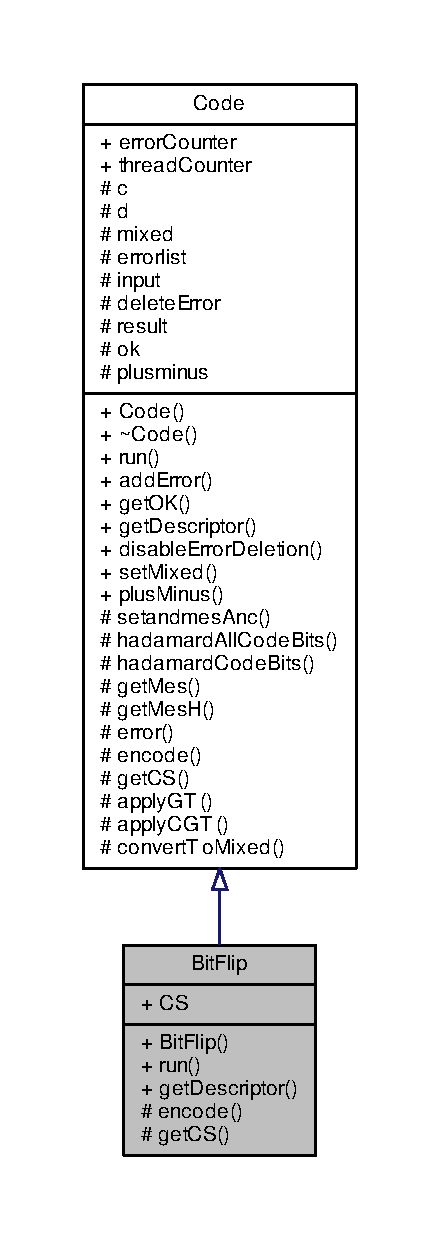
\includegraphics[height=550pt]{class_bit_flip__inherit__graph}
\end{center}
\end{figure}
\subsection*{Public Member Functions}
\begin{DoxyCompactItemize}
\item 
\hyperlink{class_bit_flip_ae5135dd8438d0c1f1d2a9d19ed753e32}{Bit\+Flip} (bool b)
\item 
bool \hyperlink{class_bit_flip_a3022463e79c6624b2123617d1957d716}{run} () override
\item 
std\+::string \hyperlink{class_bit_flip_adc65379e4eeb6eb908318a98c304e16e}{get\+Descriptor} () override
\end{DoxyCompactItemize}
\subsection*{Static Public Attributes}
\begin{DoxyCompactItemize}
\item 
static const unsigned \hyperlink{class_bit_flip_a8f5442dd93f87ea35fcb0b0bb423bbf0}{CS} = 3
\end{DoxyCompactItemize}
\subsection*{Protected Member Functions}
\begin{DoxyCompactItemize}
\item 
void \hyperlink{class_bit_flip_a45fdb2512ee2092d0c1f877afda2bb50}{encode} (bool b) override
\item 
unsigned \hyperlink{class_bit_flip_ad3c275a5fe1cb5188cb1ab3049fcfd70}{get\+CS} () override
\end{DoxyCompactItemize}
\subsection*{Additional Inherited Members}


\subsection{Detailed Description}
Bit Flip code class 

\subsection{Constructor \& Destructor Documentation}
\index{Bit\+Flip@{Bit\+Flip}!Bit\+Flip@{Bit\+Flip}}
\index{Bit\+Flip@{Bit\+Flip}!Bit\+Flip@{Bit\+Flip}}
\subsubsection[{\texorpdfstring{Bit\+Flip(bool b)}{BitFlip(bool b)}}]{\setlength{\rightskip}{0pt plus 5cm}Bit\+Flip\+::\+Bit\+Flip (
\begin{DoxyParamCaption}
\item[{bool}]{b}
\end{DoxyParamCaption}
)\hspace{0.3cm}{\ttfamily [inline]}}\hypertarget{class_bit_flip_ae5135dd8438d0c1f1d2a9d19ed753e32}{}\label{class_bit_flip_ae5135dd8438d0c1f1d2a9d19ed753e32}


\subsection{Member Function Documentation}
\index{Bit\+Flip@{Bit\+Flip}!encode@{encode}}
\index{encode@{encode}!Bit\+Flip@{Bit\+Flip}}
\subsubsection[{\texorpdfstring{encode(bool b) override}{encode(bool b) override}}]{\setlength{\rightskip}{0pt plus 5cm}void Bit\+Flip\+::encode (
\begin{DoxyParamCaption}
\item[{bool}]{b}
\end{DoxyParamCaption}
)\hspace{0.3cm}{\ttfamily [override]}, {\ttfamily [protected]}, {\ttfamily [virtual]}}\hypertarget{class_bit_flip_a45fdb2512ee2092d0c1f877afda2bb50}{}\label{class_bit_flip_a45fdb2512ee2092d0c1f877afda2bb50}
Encode input bit 
\begin{DoxyParams}{Parameters}
{\em b} & Classical input converted to $\vert$0$>$ or $\vert$1$>$ \\
\hline
\end{DoxyParams}


Implements \hyperlink{class_code_a5f90b0f96002c9b999d8ed7bab319906}{Code}.

\index{Bit\+Flip@{Bit\+Flip}!get\+CS@{get\+CS}}
\index{get\+CS@{get\+CS}!Bit\+Flip@{Bit\+Flip}}
\subsubsection[{\texorpdfstring{get\+C\+S() override}{getCS() override}}]{\setlength{\rightskip}{0pt plus 5cm}unsigned Bit\+Flip\+::get\+CS (
\begin{DoxyParamCaption}
{}
\end{DoxyParamCaption}
)\hspace{0.3cm}{\ttfamily [inline]}, {\ttfamily [override]}, {\ttfamily [protected]}, {\ttfamily [virtual]}}\hypertarget{class_bit_flip_ad3c275a5fe1cb5188cb1ab3049fcfd70}{}\label{class_bit_flip_ad3c275a5fe1cb5188cb1ab3049fcfd70}
Return code size of a child \begin{DoxyReturn}{Returns}
code size 
\end{DoxyReturn}


Implements \hyperlink{class_code_a34f52b25d78aeaec3c1fd381f025ad00}{Code}.

\index{Bit\+Flip@{Bit\+Flip}!get\+Descriptor@{get\+Descriptor}}
\index{get\+Descriptor@{get\+Descriptor}!Bit\+Flip@{Bit\+Flip}}
\subsubsection[{\texorpdfstring{get\+Descriptor() override}{getDescriptor() override}}]{\setlength{\rightskip}{0pt plus 5cm}std\+::string Bit\+Flip\+::get\+Descriptor (
\begin{DoxyParamCaption}
{}
\end{DoxyParamCaption}
)\hspace{0.3cm}{\ttfamily [override]}, {\ttfamily [virtual]}}\hypertarget{class_bit_flip_adc65379e4eeb6eb908318a98c304e16e}{}\label{class_bit_flip_adc65379e4eeb6eb908318a98c304e16e}
Returns descriptor string ~\newline
 Format\+: ~\newline
 B\+I\+T\+F\+L\+IP aa i-\/$>$o O\+K/\+E\+R\+R\+OR ~\newline
 Where aa is flip array \begin{DoxyReturn}{Returns}
Log string 
\end{DoxyReturn}


Implements \hyperlink{class_code_a60db2f615a7cff76e3ece1c486b2fd16}{Code}.

\index{Bit\+Flip@{Bit\+Flip}!run@{run}}
\index{run@{run}!Bit\+Flip@{Bit\+Flip}}
\subsubsection[{\texorpdfstring{run() override}{run() override}}]{\setlength{\rightskip}{0pt plus 5cm}bool Bit\+Flip\+::run (
\begin{DoxyParamCaption}
{}
\end{DoxyParamCaption}
)\hspace{0.3cm}{\ttfamily [override]}, {\ttfamily [virtual]}}\hypertarget{class_bit_flip_a3022463e79c6624b2123617d1957d716}{}\label{class_bit_flip_a3022463e79c6624b2123617d1957d716}
Function to simulate the transmission and get the result. To be defined in child classes. \begin{DoxyReturn}{Returns}
Measured bit at Bob 
\end{DoxyReturn}


Implements \hyperlink{class_code_a5621bbd050948ba1e41f69f451a05990}{Code}.



\subsection{Member Data Documentation}
\index{Bit\+Flip@{Bit\+Flip}!CS@{CS}}
\index{CS@{CS}!Bit\+Flip@{Bit\+Flip}}
\subsubsection[{\texorpdfstring{CS}{CS}}]{\setlength{\rightskip}{0pt plus 5cm}const unsigned Bit\+Flip\+::\+CS = 3\hspace{0.3cm}{\ttfamily [static]}}\hypertarget{class_bit_flip_a8f5442dd93f87ea35fcb0b0bb423bbf0}{}\label{class_bit_flip_a8f5442dd93f87ea35fcb0b0bb423bbf0}
\hyperlink{class_code}{Code} size for bit flip which is 3 

The documentation for this class was generated from the following files\+:\begin{DoxyCompactItemize}
\item 
/home/attila/src/qecc-\/netbeans/qecc/\hyperlink{_bit_flip_8h}{Bit\+Flip.\+h}\item 
/home/attila/src/qecc-\/netbeans/qecc/\hyperlink{_bit_flip_8cpp}{Bit\+Flip.\+cpp}\end{DoxyCompactItemize}

\hypertarget{class_channel}{}\section{Channel Class Reference}
\label{class_channel}\index{Channel@{Channel}}


{\ttfamily \#include $<$Channel.\+h$>$}

\subsection*{Public Member Functions}
\begin{DoxyCompactItemize}
\item 
\hyperlink{class_channel_a5c4f341674fed76b66ae766d268c574a}{Channel} (int nodeid0, int nodeid1, \hyperlink{class_error}{Error} $\ast$e)
\item 
bool \hyperlink{class_channel_a089e35cdef5be2b10d630c2ef4914dc1}{match\+Id} (int nid0, int nid1)
\item 
int \hyperlink{class_channel_a5b81ce0b217813d9b0ec13d5042d297f}{match\+One\+Get\+Other} (int id)
\item 
int $\ast$ \hyperlink{class_channel_adae91e67fc9e0d22d47606efe7a704ec}{get\+Ids} ()
\item 
std\+::string \hyperlink{class_channel_ac91f51b1333e8b69a936b8cd0d39bb65}{debug\+Print} ()
\item 
\hyperlink{class_error}{Error} $\ast$ \hyperlink{class_channel_a4c99f5f2b94cf100a1f91dd9df7eee81}{get\+Error} ()
\item 
\hyperlink{class_channel_a5f15ebd302464069f1a9e3f0ded14482}{$\sim$\+Channel} ()
\end{DoxyCompactItemize}


\subsection{Detailed Description}
Used by network mode ~\newline
 Stores two node ids and an error between them 

\subsection{Constructor \& Destructor Documentation}
\index{Channel@{Channel}!Channel@{Channel}}
\index{Channel@{Channel}!Channel@{Channel}}
\subsubsection[{\texorpdfstring{Channel(int nodeid0, int nodeid1, Error $\ast$e)}{Channel(int nodeid0, int nodeid1, Error *e)}}]{\setlength{\rightskip}{0pt plus 5cm}Channel\+::\+Channel (
\begin{DoxyParamCaption}
\item[{int}]{nodeid0, }
\item[{int}]{nodeid1, }
\item[{{\bf Error} $\ast$}]{e}
\end{DoxyParamCaption}
)\hspace{0.3cm}{\ttfamily [inline]}}\hypertarget{class_channel_a5c4f341674fed76b66ae766d268c574a}{}\label{class_channel_a5c4f341674fed76b66ae766d268c574a}
Constuctor 
\begin{DoxyParams}{Parameters}
{\em nodeid0} & Id of first node \\
\hline
{\em nodeid1} & Id of second node \\
\hline
{\em e} & \hyperlink{class_error}{Error} of the channel \\
\hline
\end{DoxyParams}
\index{Channel@{Channel}!````~Channel@{$\sim$\+Channel}}
\index{````~Channel@{$\sim$\+Channel}!Channel@{Channel}}
\subsubsection[{\texorpdfstring{$\sim$\+Channel()}{~Channel()}}]{\setlength{\rightskip}{0pt plus 5cm}Channel\+::$\sim$\+Channel (
\begin{DoxyParamCaption}
{}
\end{DoxyParamCaption}
)\hspace{0.3cm}{\ttfamily [inline]}}\hypertarget{class_channel_a5f15ebd302464069f1a9e3f0ded14482}{}\label{class_channel_a5f15ebd302464069f1a9e3f0ded14482}


\subsection{Member Function Documentation}
\index{Channel@{Channel}!debug\+Print@{debug\+Print}}
\index{debug\+Print@{debug\+Print}!Channel@{Channel}}
\subsubsection[{\texorpdfstring{debug\+Print()}{debugPrint()}}]{\setlength{\rightskip}{0pt plus 5cm}std\+::string Channel\+::debug\+Print (
\begin{DoxyParamCaption}
{}
\end{DoxyParamCaption}
)\hspace{0.3cm}{\ttfamily [inline]}}\hypertarget{class_channel_ac91f51b1333e8b69a936b8cd0d39bb65}{}\label{class_channel_ac91f51b1333e8b69a936b8cd0d39bb65}
Print data to string \begin{DoxyReturn}{Returns}
String which describes the instance 
\end{DoxyReturn}
\index{Channel@{Channel}!get\+Error@{get\+Error}}
\index{get\+Error@{get\+Error}!Channel@{Channel}}
\subsubsection[{\texorpdfstring{get\+Error()}{getError()}}]{\setlength{\rightskip}{0pt plus 5cm}{\bf Error}$\ast$ Channel\+::get\+Error (
\begin{DoxyParamCaption}
{}
\end{DoxyParamCaption}
)\hspace{0.3cm}{\ttfamily [inline]}}\hypertarget{class_channel_a4c99f5f2b94cf100a1f91dd9df7eee81}{}\label{class_channel_a4c99f5f2b94cf100a1f91dd9df7eee81}
Get \hyperlink{class_error}{Error} \begin{DoxyReturn}{Returns}
returns pointer to error 
\end{DoxyReturn}
\index{Channel@{Channel}!get\+Ids@{get\+Ids}}
\index{get\+Ids@{get\+Ids}!Channel@{Channel}}
\subsubsection[{\texorpdfstring{get\+Ids()}{getIds()}}]{\setlength{\rightskip}{0pt plus 5cm}int$\ast$ Channel\+::get\+Ids (
\begin{DoxyParamCaption}
{}
\end{DoxyParamCaption}
)\hspace{0.3cm}{\ttfamily [inline]}}\hypertarget{class_channel_adae91e67fc9e0d22d47606efe7a704ec}{}\label{class_channel_adae91e67fc9e0d22d47606efe7a704ec}
Get node ids \begin{DoxyReturn}{Returns}
Array of our the nodeids 
\end{DoxyReturn}
\index{Channel@{Channel}!match\+Id@{match\+Id}}
\index{match\+Id@{match\+Id}!Channel@{Channel}}
\subsubsection[{\texorpdfstring{match\+Id(int nid0, int nid1)}{matchId(int nid0, int nid1)}}]{\setlength{\rightskip}{0pt plus 5cm}bool Channel\+::match\+Id (
\begin{DoxyParamCaption}
\item[{int}]{nid0, }
\item[{int}]{nid1}
\end{DoxyParamCaption}
)\hspace{0.3cm}{\ttfamily [inline]}}\hypertarget{class_channel_a089e35cdef5be2b10d630c2ef4914dc1}{}\label{class_channel_a089e35cdef5be2b10d630c2ef4914dc1}
Check if two ids given is what we have, order does not matter 
\begin{DoxyParams}{Parameters}
{\em nid0} & First node id \\
\hline
{\em nid1} & Second node id \\
\hline
\end{DoxyParams}
\begin{DoxyReturn}{Returns}
True if our ids match the input 
\end{DoxyReturn}
\index{Channel@{Channel}!match\+One\+Get\+Other@{match\+One\+Get\+Other}}
\index{match\+One\+Get\+Other@{match\+One\+Get\+Other}!Channel@{Channel}}
\subsubsection[{\texorpdfstring{match\+One\+Get\+Other(int id)}{matchOneGetOther(int id)}}]{\setlength{\rightskip}{0pt plus 5cm}int Channel\+::match\+One\+Get\+Other (
\begin{DoxyParamCaption}
\item[{int}]{id}
\end{DoxyParamCaption}
)\hspace{0.3cm}{\ttfamily [inline]}}\hypertarget{class_channel_a5b81ce0b217813d9b0ec13d5042d297f}{}\label{class_channel_a5b81ce0b217813d9b0ec13d5042d297f}
Check if one of our ids is same as input and return the other or zero if no match 
\begin{DoxyParams}{Parameters}
{\em id} & \hyperlink{class_node}{Node} id \\
\hline
\end{DoxyParams}
\begin{DoxyReturn}{Returns}
The id of our other node on match 
\end{DoxyReturn}


The documentation for this class was generated from the following file\+:\begin{DoxyCompactItemize}
\item 
/home/attila/src/qecc-\/netbeans/qecc/\hyperlink{_channel_8h}{Channel.\+h}\end{DoxyCompactItemize}

\hypertarget{class_code}{}\section{Code Class Reference}
\label{class_code}\index{Code@{Code}}


{\ttfamily \#include $<$Code.\+h$>$}



Inheritance diagram for Code\+:
\nopagebreak
\begin{figure}[H]
\begin{center}
\leavevmode
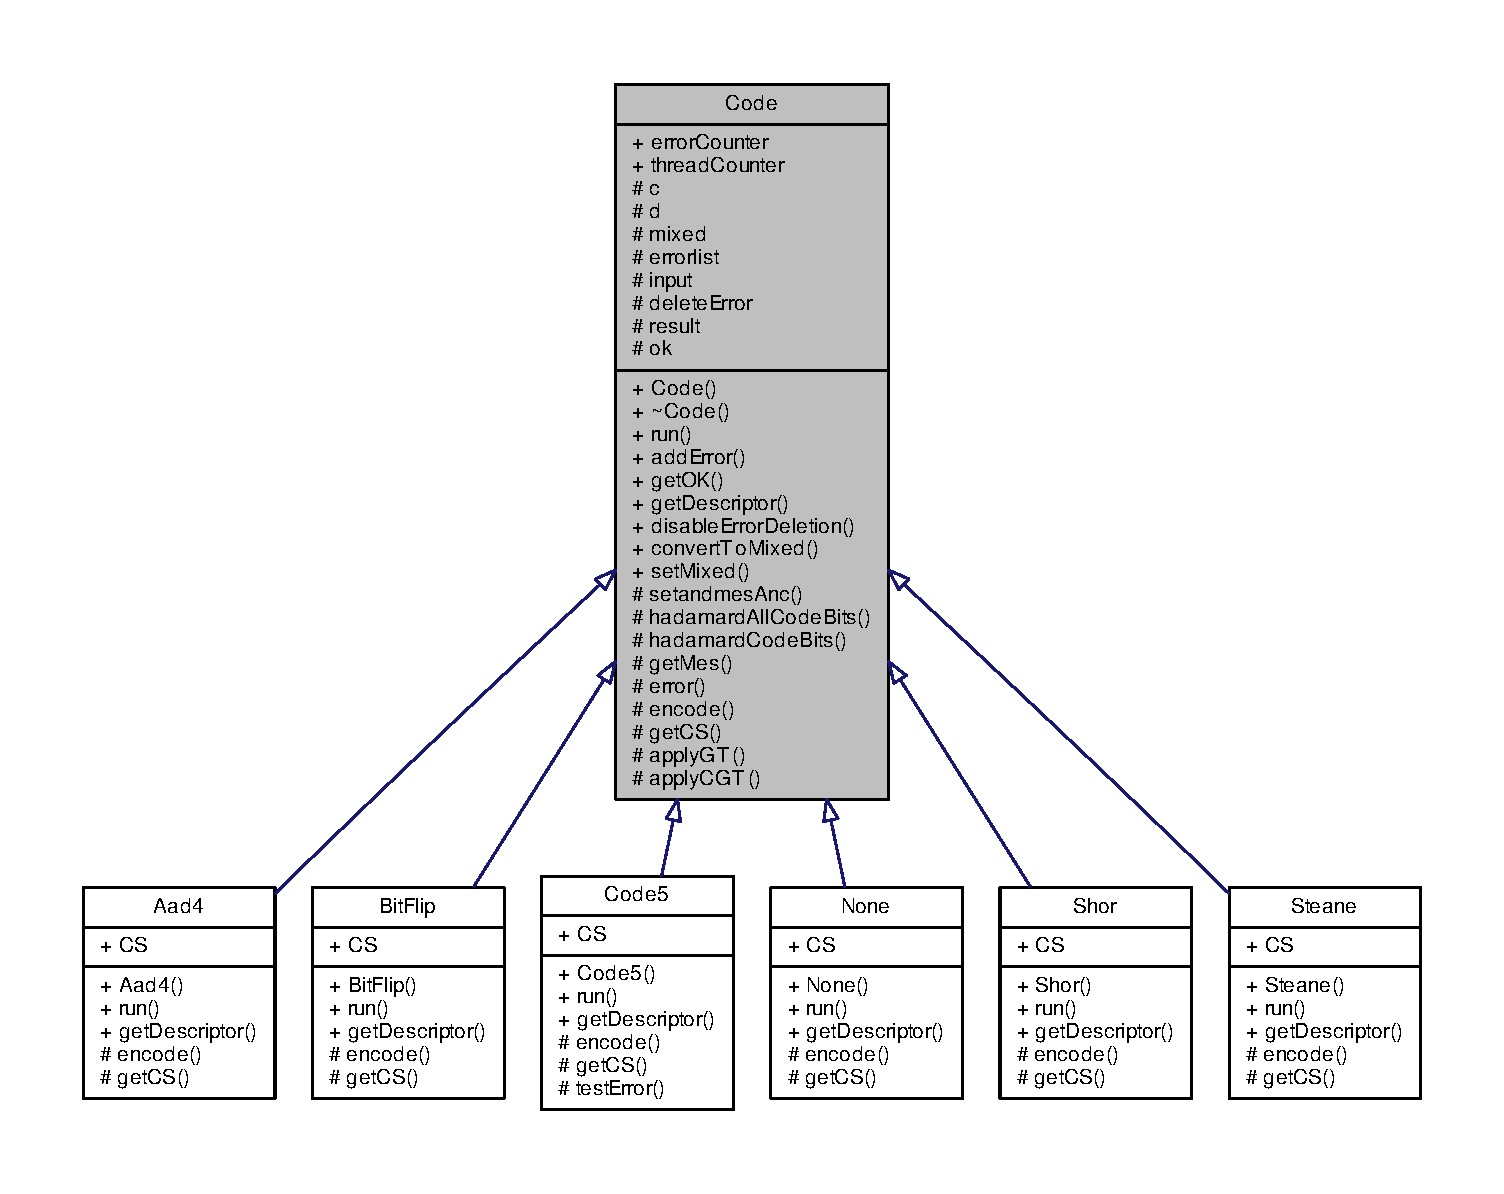
\includegraphics[width=350pt]{class_code__inherit__graph}
\end{center}
\end{figure}
\subsection*{Public Member Functions}
\begin{DoxyCompactItemize}
\item 
\hyperlink{class_code_ac37d2241363b2bfcd11db0e02d3acad6}{Code} (bool b)
\item 
virtual \hyperlink{class_code_ad9a1e323c3ed4d36aeff17faffe1e770}{$\sim$\+Code} ()
\item 
virtual bool \hyperlink{class_code_a5621bbd050948ba1e41f69f451a05990}{run} ()=0
\item 
void \hyperlink{class_code_a79f6282eeac2d8c2d61bab55ddf2e797}{add\+Error} (\hyperlink{class_error}{Error} $\ast$e)
\item 
bool \hyperlink{class_code_a6a7ff74d4db8bc010c750afa1f1743c1}{get\+OK} ()
\item 
virtual std\+::string \hyperlink{class_code_a60db2f615a7cff76e3ece1c486b2fd16}{get\+Descriptor} ()=0
\item 
void \hyperlink{class_code_a58a0c6a1b046c6d20703d32c6a7fefbc}{disable\+Error\+Deletion} ()
\item 
void \hyperlink{class_code_a85f5a2e8133b68173334f24d66f4d5a9}{set\+Mixed} ()
\item 
void \hyperlink{class_code_ac4248e25a1ca509c128ec236be57c946}{plus\+Minus} ()
\end{DoxyCompactItemize}
\subsection*{Public Attributes}
\begin{DoxyCompactItemize}
\item 
std\+::atomic\+\_\+int $\ast$ \hyperlink{class_code_ab4f00a8ff5a23276a54c7b163b34219a}{error\+Counter}
\item 
std\+::atomic\+\_\+int $\ast$ \hyperlink{class_code_a3c6a29ddf07c39bda3e78d05cada42b5}{thread\+Counter}
\end{DoxyCompactItemize}
\subsection*{Protected Member Functions}
\begin{DoxyCompactItemize}
\item 
bool \hyperlink{class_code_a30cba39121d9b63fd3344f639fe42487}{setandmes\+Anc} (const std\+::vector$<$ unsigned $>$ \&b, unsigned CS)
\item 
void \hyperlink{class_code_ad554df1048f44e7e02404e9670a3d8de}{hadamard\+All\+Code\+Bits} ()
\item 
void \hyperlink{class_code_ac67d0cdd389466240874cc124137b6ac}{hadamard\+Code\+Bits} (const std\+::vector$<$ unsigned $>$ \&b)
\item 
bool \hyperlink{class_code_ac1116dcd1573b570cfee1a044f4526a9}{get\+Mes} (unsigned i)
\item 
bool \hyperlink{class_code_a080e5bd0105b1f02a5c3568b01a7758a}{get\+MesH} (unsigned i)
\item 
void \hyperlink{class_code_af87289ca8b76769d7a572a0d1b324155}{error} ()
\item 
virtual void \hyperlink{class_code_a5f90b0f96002c9b999d8ed7bab319906}{encode} (bool b)=0
\item 
virtual unsigned \hyperlink{class_code_a34f52b25d78aeaec3c1fd381f025ad00}{get\+CS} ()=0
\item 
void \hyperlink{class_code_a63474ffa6825d0efcfa8a40cac225d4a}{apply\+GT} (const cmat gate, unsigned b)
\item 
void \hyperlink{class_code_a3fe9fc7acd3f4c9cc80d5fd39322ca04}{apply\+C\+GT} (const cmat gate, const std\+::vector$<$ unsigned $>$ \&b)
\item 
void \hyperlink{class_code_ae26ecba630093dcac2b7c01946678cb0}{convert\+To\+Mixed} ()
\end{DoxyCompactItemize}
\subsection*{Protected Attributes}
\begin{DoxyCompactItemize}
\item 
ket $\ast$ \hyperlink{class_code_a01a6ba9da79914bc6980ffddf53ecb24}{c}
\item 
cmat $\ast$ \hyperlink{class_code_a92025265fbd17156f2a3dc7a6e5364f6}{d}
\item 
bool \hyperlink{class_code_a299e61614fc7ae8e3cbcba232d57d042}{mixed}
\item 
std\+::queue$<$ \hyperlink{class_error}{Error} $\ast$ $>$ \hyperlink{class_code_a8eed999145874a4fe25c8a3ad589d225}{errorlist}
\item 
bool \hyperlink{class_code_a0bdc22fcdc5b2a78a8ace1aea2d96d34}{input}
\item 
bool \hyperlink{class_code_ae448fe74faf959e28ae7a17d13dd4790}{delete\+Error}
\item 
bool \hyperlink{class_code_ac65cd5a89311ea1059ba7d3772d812f9}{result}
\item 
bool \hyperlink{class_code_a62ce9f737b915662364116664261969a}{ok}
\item 
bool \hyperlink{class_code_abd650233920e3b6778032b7d58282976}{plusminus}
\end{DoxyCompactItemize}
\subsection*{Friends}
\begin{DoxyCompactItemize}
\item 
class \hyperlink{class_code_a16d3937baa3679c525821223427be40b}{Error}
\end{DoxyCompactItemize}


\subsection{Detailed Description}
\hyperlink{class_code}{Code} class is provides a way to simulate a code on an erroneous channel ~\newline
 This is the parent of all specific code classes 

\subsection{Constructor \& Destructor Documentation}
\index{Code@{Code}!Code@{Code}}
\index{Code@{Code}!Code@{Code}}
\subsubsection[{\texorpdfstring{Code(bool b)}{Code(bool b)}}]{\setlength{\rightskip}{0pt plus 5cm}Code\+::\+Code (
\begin{DoxyParamCaption}
\item[{bool}]{b}
\end{DoxyParamCaption}
)}\hypertarget{class_code_ac37d2241363b2bfcd11db0e02d3acad6}{}\label{class_code_ac37d2241363b2bfcd11db0e02d3acad6}
Constructor 
\begin{DoxyParams}{Parameters}
{\em b} & Input bit 1 or 0 \\
\hline
\end{DoxyParams}
\index{Code@{Code}!````~Code@{$\sim$\+Code}}
\index{````~Code@{$\sim$\+Code}!Code@{Code}}
\subsubsection[{\texorpdfstring{$\sim$\+Code()}{~Code()}}]{\setlength{\rightskip}{0pt plus 5cm}Code\+::$\sim$\+Code (
\begin{DoxyParamCaption}
{}
\end{DoxyParamCaption}
)\hspace{0.3cm}{\ttfamily [virtual]}}\hypertarget{class_code_ad9a1e323c3ed4d36aeff17faffe1e770}{}\label{class_code_ad9a1e323c3ed4d36aeff17faffe1e770}
Destructor 

\subsection{Member Function Documentation}
\index{Code@{Code}!add\+Error@{add\+Error}}
\index{add\+Error@{add\+Error}!Code@{Code}}
\subsubsection[{\texorpdfstring{add\+Error(\+Error $\ast$e)}{addError(Error *e)}}]{\setlength{\rightskip}{0pt plus 5cm}void Code\+::add\+Error (
\begin{DoxyParamCaption}
\item[{{\bf Error} $\ast$}]{e}
\end{DoxyParamCaption}
)\hspace{0.3cm}{\ttfamily [inline]}}\hypertarget{class_code_a79f6282eeac2d8c2d61bab55ddf2e797}{}\label{class_code_a79f6282eeac2d8c2d61bab55ddf2e797}
Add an error to the error list 
\begin{DoxyParams}{Parameters}
{\em e} & Pointer to an error to be added \\
\hline
\end{DoxyParams}
\index{Code@{Code}!apply\+C\+GT@{apply\+C\+GT}}
\index{apply\+C\+GT@{apply\+C\+GT}!Code@{Code}}
\subsubsection[{\texorpdfstring{apply\+C\+G\+T(const cmat gate, const std\+::vector$<$ unsigned $>$ \&b)}{applyCGT(const cmat gate, const std::vector< unsigned > &b)}}]{\setlength{\rightskip}{0pt plus 5cm}void Code\+::apply\+C\+GT (
\begin{DoxyParamCaption}
\item[{const cmat}]{gate, }
\item[{const std\+::vector$<$ unsigned $>$ \&}]{b}
\end{DoxyParamCaption}
)\hspace{0.3cm}{\ttfamily [inline]}, {\ttfamily [protected]}}\hypertarget{class_code_a3fe9fc7acd3f4c9cc80d5fd39322ca04}{}\label{class_code_a3fe9fc7acd3f4c9cc80d5fd39322ca04}
Applies a 2 qubit gate 
\begin{DoxyParams}{Parameters}
{\em gate} & Matrix of the gate \\
\hline
{\em b} & array of two subsystem ids \\
\hline
\end{DoxyParams}
\index{Code@{Code}!apply\+GT@{apply\+GT}}
\index{apply\+GT@{apply\+GT}!Code@{Code}}
\subsubsection[{\texorpdfstring{apply\+G\+T(const cmat gate, unsigned b)}{applyGT(const cmat gate, unsigned b)}}]{\setlength{\rightskip}{0pt plus 5cm}void Code\+::apply\+GT (
\begin{DoxyParamCaption}
\item[{const cmat}]{gate, }
\item[{unsigned}]{b}
\end{DoxyParamCaption}
)\hspace{0.3cm}{\ttfamily [inline]}, {\ttfamily [protected]}}\hypertarget{class_code_a63474ffa6825d0efcfa8a40cac225d4a}{}\label{class_code_a63474ffa6825d0efcfa8a40cac225d4a}
Applies a single qubit gate 
\begin{DoxyParams}{Parameters}
{\em gate} & Matrix of the gate \\
\hline
{\em b} & subsystem id \\
\hline
\end{DoxyParams}
\index{Code@{Code}!convert\+To\+Mixed@{convert\+To\+Mixed}}
\index{convert\+To\+Mixed@{convert\+To\+Mixed}!Code@{Code}}
\subsubsection[{\texorpdfstring{convert\+To\+Mixed()}{convertToMixed()}}]{\setlength{\rightskip}{0pt plus 5cm}void Code\+::convert\+To\+Mixed (
\begin{DoxyParamCaption}
{}
\end{DoxyParamCaption}
)\hspace{0.3cm}{\ttfamily [inline]}, {\ttfamily [protected]}}\hypertarget{class_code_ae26ecba630093dcac2b7c01946678cb0}{}\label{class_code_ae26ecba630093dcac2b7c01946678cb0}
Convert vector notation to density matrix. {\bfseries Must be called inside run!} From outside class stays the same but inside it will use density matrix. This has a performance drawback but needed for some errors for example amplitude damping. An amplitude damping \hyperlink{class_error}{Error} does this conversion automatically. \index{Code@{Code}!disable\+Error\+Deletion@{disable\+Error\+Deletion}}
\index{disable\+Error\+Deletion@{disable\+Error\+Deletion}!Code@{Code}}
\subsubsection[{\texorpdfstring{disable\+Error\+Deletion()}{disableErrorDeletion()}}]{\setlength{\rightskip}{0pt plus 5cm}void Code\+::disable\+Error\+Deletion (
\begin{DoxyParamCaption}
{}
\end{DoxyParamCaption}
)\hspace{0.3cm}{\ttfamily [inline]}}\hypertarget{class_code_a58a0c6a1b046c6d20703d32c6a7fefbc}{}\label{class_code_a58a0c6a1b046c6d20703d32c6a7fefbc}
Normally Errors are deleted by run function. If the given \hyperlink{class_error}{Error} instance is being used by multiple \hyperlink{class_code}{Code} instances this will disable deletion of it . \index{Code@{Code}!encode@{encode}}
\index{encode@{encode}!Code@{Code}}
\subsubsection[{\texorpdfstring{encode(bool b)=0}{encode(bool b)=0}}]{\setlength{\rightskip}{0pt plus 5cm}virtual void Code\+::encode (
\begin{DoxyParamCaption}
\item[{bool}]{b}
\end{DoxyParamCaption}
)\hspace{0.3cm}{\ttfamily [protected]}, {\ttfamily [pure virtual]}}\hypertarget{class_code_a5f90b0f96002c9b999d8ed7bab319906}{}\label{class_code_a5f90b0f96002c9b999d8ed7bab319906}
Encode input bit 
\begin{DoxyParams}{Parameters}
{\em b} & Classical input converted to $\vert$0$>$ or $\vert$1$>$ \\
\hline
\end{DoxyParams}


Implemented in \hyperlink{class_code5_a17456381dabab2ba1b28bf232376908f}{Code5}, \hyperlink{class_shor_a77db4d99076a0e581057faae8071574c}{Shor}, \hyperlink{class_none_a5f7b2a6913822dff79ce6d90b7428ecc}{None}, \hyperlink{class_steane_a3c64f20d7329b609984f115cd35651ab}{Steane}, \hyperlink{class_bit_flip_a45fdb2512ee2092d0c1f877afda2bb50}{Bit\+Flip}, and \hyperlink{class_aad4_ad3febfa430563be08f78c3b7e8517ff6}{Aad4}.

\index{Code@{Code}!error@{error}}
\index{error@{error}!Code@{Code}}
\subsubsection[{\texorpdfstring{error()}{error()}}]{\setlength{\rightskip}{0pt plus 5cm}void Code\+::error (
\begin{DoxyParamCaption}
{}
\end{DoxyParamCaption}
)\hspace{0.3cm}{\ttfamily [protected]}}\hypertarget{class_code_af87289ca8b76769d7a572a0d1b324155}{}\label{class_code_af87289ca8b76769d7a572a0d1b324155}
Applies errors on c or d \index{Code@{Code}!get\+CS@{get\+CS}}
\index{get\+CS@{get\+CS}!Code@{Code}}
\subsubsection[{\texorpdfstring{get\+C\+S()=0}{getCS()=0}}]{\setlength{\rightskip}{0pt plus 5cm}virtual unsigned Code\+::get\+CS (
\begin{DoxyParamCaption}
{}
\end{DoxyParamCaption}
)\hspace{0.3cm}{\ttfamily [protected]}, {\ttfamily [pure virtual]}}\hypertarget{class_code_a34f52b25d78aeaec3c1fd381f025ad00}{}\label{class_code_a34f52b25d78aeaec3c1fd381f025ad00}
Return code size of a child \begin{DoxyReturn}{Returns}
code size 
\end{DoxyReturn}


Implemented in \hyperlink{class_code5_a518d2eb49ea82e92b74458db5477abf6}{Code5}, \hyperlink{class_shor_a5cfb32ea0c6f73fd9478ce93b7fafb4f}{Shor}, \hyperlink{class_none_a6e8b66f3489dbc5e1b231c27534c484d}{None}, \hyperlink{class_steane_a7b84b86f9d9737890a146e11479683e6}{Steane}, \hyperlink{class_bit_flip_ad3c275a5fe1cb5188cb1ab3049fcfd70}{Bit\+Flip}, and \hyperlink{class_aad4_af4cb779e50399fcdca7a2f62282b7e78}{Aad4}.

\index{Code@{Code}!get\+Descriptor@{get\+Descriptor}}
\index{get\+Descriptor@{get\+Descriptor}!Code@{Code}}
\subsubsection[{\texorpdfstring{get\+Descriptor()=0}{getDescriptor()=0}}]{\setlength{\rightskip}{0pt plus 5cm}virtual std\+::string Code\+::get\+Descriptor (
\begin{DoxyParamCaption}
{}
\end{DoxyParamCaption}
)\hspace{0.3cm}{\ttfamily [pure virtual]}}\hypertarget{class_code_a60db2f615a7cff76e3ece1c486b2fd16}{}\label{class_code_a60db2f615a7cff76e3ece1c486b2fd16}
Log of run ~\newline
 To be defined in child class ~\newline
 Contains code type, input, output, ancilla bit measurements ~\newline
 Format\+:~\newline
 {\itshape C\+O\+D\+E\+T\+Y\+PE ancillas input-\/$>$result O\+K/\+E\+R\+R\+OR} \begin{DoxyReturn}{Returns}
log string 
\end{DoxyReturn}


Implemented in \hyperlink{class_code5_ab7cd6f3c172a4a0c45bc0fa41a3ff535}{Code5}, \hyperlink{class_shor_ad9a43efd28edf5df378d0c6b7dfbb051}{Shor}, \hyperlink{class_none_a0ad5c4d177835a8fc0498d606fefbd79}{None}, \hyperlink{class_steane_a1fb53da78a66d64cd6aad02735fab4c3}{Steane}, \hyperlink{class_bit_flip_adc65379e4eeb6eb908318a98c304e16e}{Bit\+Flip}, and \hyperlink{class_aad4_ad697e56ab152cd1228bd26f73451ec42}{Aad4}.

\index{Code@{Code}!get\+Mes@{get\+Mes}}
\index{get\+Mes@{get\+Mes}!Code@{Code}}
\subsubsection[{\texorpdfstring{get\+Mes(unsigned i)}{getMes(unsigned i)}}]{\setlength{\rightskip}{0pt plus 5cm}bool Code\+::get\+Mes (
\begin{DoxyParamCaption}
\item[{unsigned}]{i}
\end{DoxyParamCaption}
)\hspace{0.3cm}{\ttfamily [protected]}}\hypertarget{class_code_ac1116dcd1573b570cfee1a044f4526a9}{}\label{class_code_ac1116dcd1573b570cfee1a044f4526a9}
Measures bit 
\begin{DoxyParams}{Parameters}
{\em i} & Subsystem id \\
\hline
\end{DoxyParams}
\begin{DoxyReturn}{Returns}
Measured classical value 
\end{DoxyReturn}
\index{Code@{Code}!get\+MesH@{get\+MesH}}
\index{get\+MesH@{get\+MesH}!Code@{Code}}
\subsubsection[{\texorpdfstring{get\+Mes\+H(unsigned i)}{getMesH(unsigned i)}}]{\setlength{\rightskip}{0pt plus 5cm}bool Code\+::get\+MesH (
\begin{DoxyParamCaption}
\item[{unsigned}]{i}
\end{DoxyParamCaption}
)\hspace{0.3cm}{\ttfamily [protected]}}\hypertarget{class_code_a080e5bd0105b1f02a5c3568b01a7758a}{}\label{class_code_a080e5bd0105b1f02a5c3568b01a7758a}
\index{Code@{Code}!get\+OK@{get\+OK}}
\index{get\+OK@{get\+OK}!Code@{Code}}
\subsubsection[{\texorpdfstring{get\+O\+K()}{getOK()}}]{\setlength{\rightskip}{0pt plus 5cm}bool Code\+::get\+OK (
\begin{DoxyParamCaption}
{}
\end{DoxyParamCaption}
)\hspace{0.3cm}{\ttfamily [inline]}}\hypertarget{class_code_a6a7ff74d4db8bc010c750afa1f1743c1}{}\label{class_code_a6a7ff74d4db8bc010c750afa1f1743c1}
Check whether transmission was successful \begin{DoxyReturn}{Returns}
True if input is same as result, false if otherwise 
\end{DoxyReturn}
\index{Code@{Code}!hadamard\+All\+Code\+Bits@{hadamard\+All\+Code\+Bits}}
\index{hadamard\+All\+Code\+Bits@{hadamard\+All\+Code\+Bits}!Code@{Code}}
\subsubsection[{\texorpdfstring{hadamard\+All\+Code\+Bits()}{hadamardAllCodeBits()}}]{\setlength{\rightskip}{0pt plus 5cm}void Code\+::hadamard\+All\+Code\+Bits (
\begin{DoxyParamCaption}
{}
\end{DoxyParamCaption}
)\hspace{0.3cm}{\ttfamily [protected]}}\hypertarget{class_code_ad554df1048f44e7e02404e9670a3d8de}{}\label{class_code_ad554df1048f44e7e02404e9670a3d8de}
Hadamard transforms all codebits \index{Code@{Code}!hadamard\+Code\+Bits@{hadamard\+Code\+Bits}}
\index{hadamard\+Code\+Bits@{hadamard\+Code\+Bits}!Code@{Code}}
\subsubsection[{\texorpdfstring{hadamard\+Code\+Bits(const std\+::vector$<$ unsigned $>$ \&b)}{hadamardCodeBits(const std::vector< unsigned > &b)}}]{\setlength{\rightskip}{0pt plus 5cm}void Code\+::hadamard\+Code\+Bits (
\begin{DoxyParamCaption}
\item[{const std\+::vector$<$ unsigned $>$ \&}]{b}
\end{DoxyParamCaption}
)\hspace{0.3cm}{\ttfamily [protected]}}\hypertarget{class_code_ac67d0cdd389466240874cc124137b6ac}{}\label{class_code_ac67d0cdd389466240874cc124137b6ac}
Hadamard transforms a set of codebits 
\begin{DoxyParams}{Parameters}
{\em b} & Bits to transform \\
\hline
\end{DoxyParams}
\index{Code@{Code}!plus\+Minus@{plus\+Minus}}
\index{plus\+Minus@{plus\+Minus}!Code@{Code}}
\subsubsection[{\texorpdfstring{plus\+Minus()}{plusMinus()}}]{\setlength{\rightskip}{0pt plus 5cm}void Code\+::plus\+Minus (
\begin{DoxyParamCaption}
{}
\end{DoxyParamCaption}
)\hspace{0.3cm}{\ttfamily [inline]}}\hypertarget{class_code_ac4248e25a1ca509c128ec236be57c946}{}\label{class_code_ac4248e25a1ca509c128ec236be57c946}
Run code in ket+, ket-\/ basis \index{Code@{Code}!run@{run}}
\index{run@{run}!Code@{Code}}
\subsubsection[{\texorpdfstring{run()=0}{run()=0}}]{\setlength{\rightskip}{0pt plus 5cm}virtual bool Code\+::run (
\begin{DoxyParamCaption}
{}
\end{DoxyParamCaption}
)\hspace{0.3cm}{\ttfamily [pure virtual]}}\hypertarget{class_code_a5621bbd050948ba1e41f69f451a05990}{}\label{class_code_a5621bbd050948ba1e41f69f451a05990}
Function to simulate the transmission and get the result. To be defined in child classes. \begin{DoxyReturn}{Returns}
Measured bit at Bob 
\end{DoxyReturn}


Implemented in \hyperlink{class_code5_ad2aec9994037880f38205e739a8f8a4a}{Code5}, \hyperlink{class_shor_abe454e38fed6f33d832c3d7fd64627ea}{Shor}, \hyperlink{class_none_aa8386e7d54637a7fd089bb84b5518c9d}{None}, \hyperlink{class_steane_a0d891a1213b62e1b225fab265fab3fc9}{Steane}, \hyperlink{class_bit_flip_a3022463e79c6624b2123617d1957d716}{Bit\+Flip}, and \hyperlink{class_aad4_a95f5ec483584c48bde0fd96d4d347c34}{Aad4}.

\index{Code@{Code}!setandmes\+Anc@{setandmes\+Anc}}
\index{setandmes\+Anc@{setandmes\+Anc}!Code@{Code}}
\subsubsection[{\texorpdfstring{setandmes\+Anc(const std\+::vector$<$ unsigned $>$ \&b, unsigned C\+S)}{setandmesAnc(const std::vector< unsigned > &b, unsigned CS)}}]{\setlength{\rightskip}{0pt plus 5cm}bool Code\+::setandmes\+Anc (
\begin{DoxyParamCaption}
\item[{const std\+::vector$<$ unsigned $>$ \&}]{b, }
\item[{unsigned}]{CS}
\end{DoxyParamCaption}
)\hspace{0.3cm}{\ttfamily [protected]}}\hypertarget{class_code_a30cba39121d9b63fd3344f639fe42487}{}\label{class_code_a30cba39121d9b63fd3344f639fe42487}
Applies C\+N\+OT gates controlled by bits in b on ancilla one-\/by-\/one. Than measures ancilla and returns its classical value. 
\begin{DoxyParams}{Parameters}
{\em b} & Bits controlling ancilla \\
\hline
{\em CS} & \hyperlink{class_code}{Code} size \\
\hline
\end{DoxyParams}
\begin{DoxyReturn}{Returns}
Classical value of ancilla 
\end{DoxyReturn}
\index{Code@{Code}!set\+Mixed@{set\+Mixed}}
\index{set\+Mixed@{set\+Mixed}!Code@{Code}}
\subsubsection[{\texorpdfstring{set\+Mixed()}{setMixed()}}]{\setlength{\rightskip}{0pt plus 5cm}void Code\+::set\+Mixed (
\begin{DoxyParamCaption}
{}
\end{DoxyParamCaption}
)\hspace{0.3cm}{\ttfamily [inline]}}\hypertarget{class_code_a85f5a2e8133b68173334f24d66f4d5a9}{}\label{class_code_a85f5a2e8133b68173334f24d66f4d5a9}
Converts vector notation to density matrix. {\bfseries Must be called before run!} Useful for testing. 

\subsection{Friends And Related Function Documentation}
\index{Code@{Code}!Error@{Error}}
\index{Error@{Error}!Code@{Code}}
\subsubsection[{\texorpdfstring{Error}{Error}}]{\setlength{\rightskip}{0pt plus 5cm}friend class {\bf Error}\hspace{0.3cm}{\ttfamily [friend]}}\hypertarget{class_code_a16d3937baa3679c525821223427be40b}{}\label{class_code_a16d3937baa3679c525821223427be40b}


\subsection{Member Data Documentation}
\index{Code@{Code}!c@{c}}
\index{c@{c}!Code@{Code}}
\subsubsection[{\texorpdfstring{c}{c}}]{\setlength{\rightskip}{0pt plus 5cm}ket$\ast$ Code\+::c\hspace{0.3cm}{\ttfamily [protected]}}\hypertarget{class_code_a01a6ba9da79914bc6980ffddf53ecb24}{}\label{class_code_a01a6ba9da79914bc6980ffddf53ecb24}
Contains state in vector notation \index{Code@{Code}!d@{d}}
\index{d@{d}!Code@{Code}}
\subsubsection[{\texorpdfstring{d}{d}}]{\setlength{\rightskip}{0pt plus 5cm}cmat$\ast$ Code\+::d\hspace{0.3cm}{\ttfamily [protected]}}\hypertarget{class_code_a92025265fbd17156f2a3dc7a6e5364f6}{}\label{class_code_a92025265fbd17156f2a3dc7a6e5364f6}
Contains state in density matrix \index{Code@{Code}!delete\+Error@{delete\+Error}}
\index{delete\+Error@{delete\+Error}!Code@{Code}}
\subsubsection[{\texorpdfstring{delete\+Error}{deleteError}}]{\setlength{\rightskip}{0pt plus 5cm}bool Code\+::delete\+Error\hspace{0.3cm}{\ttfamily [protected]}}\hypertarget{class_code_ae448fe74faf959e28ae7a17d13dd4790}{}\label{class_code_ae448fe74faf959e28ae7a17d13dd4790}
Delete Errors on run. True by default. \index{Code@{Code}!error\+Counter@{error\+Counter}}
\index{error\+Counter@{error\+Counter}!Code@{Code}}
\subsubsection[{\texorpdfstring{error\+Counter}{errorCounter}}]{\setlength{\rightskip}{0pt plus 5cm}std\+::atomic\+\_\+int$\ast$ Code\+::error\+Counter}\hypertarget{class_code_ab4f00a8ff5a23276a54c7b163b34219a}{}\label{class_code_ab4f00a8ff5a23276a54c7b163b34219a}
External error counter provided by \hyperlink{class_runner}{Runner} class. If an error occurs this is incremented. \index{Code@{Code}!errorlist@{errorlist}}
\index{errorlist@{errorlist}!Code@{Code}}
\subsubsection[{\texorpdfstring{errorlist}{errorlist}}]{\setlength{\rightskip}{0pt plus 5cm}std\+::queue$<${\bf Error} $\ast$$>$ Code\+::errorlist\hspace{0.3cm}{\ttfamily [protected]}}\hypertarget{class_code_a8eed999145874a4fe25c8a3ad589d225}{}\label{class_code_a8eed999145874a4fe25c8a3ad589d225}
List of errors to be applied \index{Code@{Code}!input@{input}}
\index{input@{input}!Code@{Code}}
\subsubsection[{\texorpdfstring{input}{input}}]{\setlength{\rightskip}{0pt plus 5cm}bool Code\+::input\hspace{0.3cm}{\ttfamily [protected]}}\hypertarget{class_code_a0bdc22fcdc5b2a78a8ace1aea2d96d34}{}\label{class_code_a0bdc22fcdc5b2a78a8ace1aea2d96d34}
Input bit, converted to $\vert$0$>$ or $\vert$1$>$ \index{Code@{Code}!mixed@{mixed}}
\index{mixed@{mixed}!Code@{Code}}
\subsubsection[{\texorpdfstring{mixed}{mixed}}]{\setlength{\rightskip}{0pt plus 5cm}bool Code\+::mixed\hspace{0.3cm}{\ttfamily [protected]}}\hypertarget{class_code_a299e61614fc7ae8e3cbcba232d57d042}{}\label{class_code_a299e61614fc7ae8e3cbcba232d57d042}
True if density matrix is used \index{Code@{Code}!ok@{ok}}
\index{ok@{ok}!Code@{Code}}
\subsubsection[{\texorpdfstring{ok}{ok}}]{\setlength{\rightskip}{0pt plus 5cm}bool Code\+::ok\hspace{0.3cm}{\ttfamily [protected]}}\hypertarget{class_code_a62ce9f737b915662364116664261969a}{}\label{class_code_a62ce9f737b915662364116664261969a}
True if result is same as input, false otherwise \index{Code@{Code}!plusminus@{plusminus}}
\index{plusminus@{plusminus}!Code@{Code}}
\subsubsection[{\texorpdfstring{plusminus}{plusminus}}]{\setlength{\rightskip}{0pt plus 5cm}bool Code\+::plusminus\hspace{0.3cm}{\ttfamily [protected]}}\hypertarget{class_code_abd650233920e3b6778032b7d58282976}{}\label{class_code_abd650233920e3b6778032b7d58282976}
Run code in ket+, ket-\/ basis \index{Code@{Code}!result@{result}}
\index{result@{result}!Code@{Code}}
\subsubsection[{\texorpdfstring{result}{result}}]{\setlength{\rightskip}{0pt plus 5cm}bool Code\+::result\hspace{0.3cm}{\ttfamily [protected]}}\hypertarget{class_code_ac65cd5a89311ea1059ba7d3772d812f9}{}\label{class_code_ac65cd5a89311ea1059ba7d3772d812f9}
Measured bit, being set by run \index{Code@{Code}!thread\+Counter@{thread\+Counter}}
\index{thread\+Counter@{thread\+Counter}!Code@{Code}}
\subsubsection[{\texorpdfstring{thread\+Counter}{threadCounter}}]{\setlength{\rightskip}{0pt plus 5cm}std\+::atomic\+\_\+int$\ast$ Code\+::thread\+Counter}\hypertarget{class_code_a3c6a29ddf07c39bda3e78d05cada42b5}{}\label{class_code_a3c6a29ddf07c39bda3e78d05cada42b5}
Thread counter of \hyperlink{class_runner}{Runner} class. After run \hyperlink{class_runner}{Runner} decrements this. 

The documentation for this class was generated from the following files\+:\begin{DoxyCompactItemize}
\item 
/home/attila/src/qecc-\/netbeans/qecc/\hyperlink{_code_8h}{Code.\+h}\item 
/home/attila/src/qecc-\/netbeans/qecc/\hyperlink{_code_8cpp}{Code.\+cpp}\end{DoxyCompactItemize}

\hypertarget{class_code5}{}\section{Code5 Class Reference}
\label{class_code5}\index{Code5@{Code5}}


{\ttfamily \#include $<$Code5.\+h$>$}



Inheritance diagram for Code5\+:
\nopagebreak
\begin{figure}[H]
\begin{center}
\leavevmode
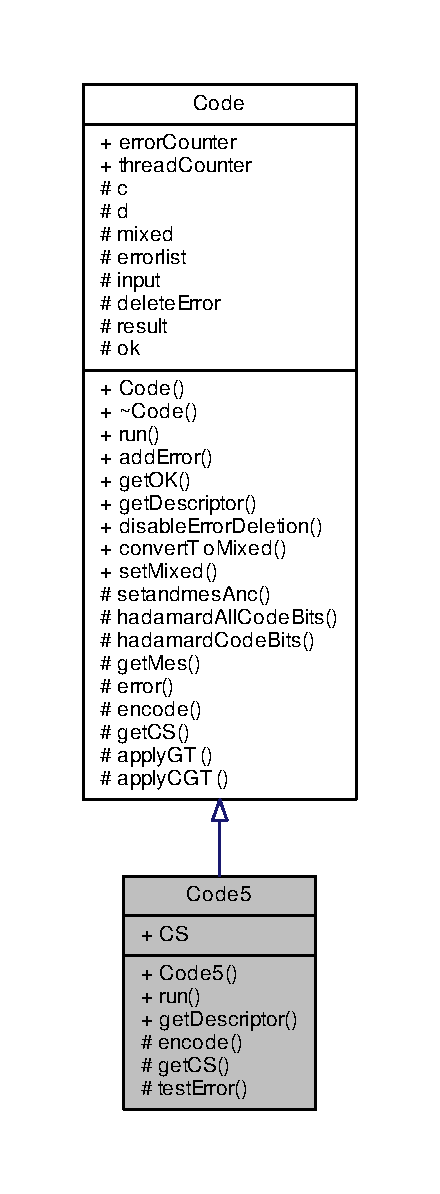
\includegraphics[height=550pt]{class_code5__inherit__graph}
\end{center}
\end{figure}
\subsection*{Public Member Functions}
\begin{DoxyCompactItemize}
\item 
\hyperlink{class_code5_ae98c6fa8281984fdc2f78e7d989a8664}{Code5} (bool b)
\item 
bool \hyperlink{class_code5_ad2aec9994037880f38205e739a8f8a4a}{run} () override
\item 
std\+::string \hyperlink{class_code5_ab7cd6f3c172a4a0c45bc0fa41a3ff535}{get\+Descriptor} () override
\end{DoxyCompactItemize}
\subsection*{Static Public Attributes}
\begin{DoxyCompactItemize}
\item 
static const unsigned \hyperlink{class_code5_ac252f1c41568341657456564d0417630}{CS} = 5
\end{DoxyCompactItemize}
\subsection*{Protected Member Functions}
\begin{DoxyCompactItemize}
\item 
void \hyperlink{class_code5_a17456381dabab2ba1b28bf232376908f}{encode} (bool b) override
\item 
unsigned \hyperlink{class_code5_a518d2eb49ea82e92b74458db5477abf6}{get\+CS} () override
\item 
void \hyperlink{class_code5_aadf204a584266bdf5bbb860191ed7c2a}{test\+Error} ()
\end{DoxyCompactItemize}
\subsection*{Additional Inherited Members}


\subsection{Detailed Description}
5\+Qubit code class 

\subsection{Constructor \& Destructor Documentation}
\index{Code5@{Code5}!Code5@{Code5}}
\index{Code5@{Code5}!Code5@{Code5}}
\subsubsection[{\texorpdfstring{Code5(bool b)}{Code5(bool b)}}]{\setlength{\rightskip}{0pt plus 5cm}Code5\+::\+Code5 (
\begin{DoxyParamCaption}
\item[{bool}]{b}
\end{DoxyParamCaption}
)\hspace{0.3cm}{\ttfamily [inline]}}\hypertarget{class_code5_ae98c6fa8281984fdc2f78e7d989a8664}{}\label{class_code5_ae98c6fa8281984fdc2f78e7d989a8664}


\subsection{Member Function Documentation}
\index{Code5@{Code5}!encode@{encode}}
\index{encode@{encode}!Code5@{Code5}}
\subsubsection[{\texorpdfstring{encode(bool b) override}{encode(bool b) override}}]{\setlength{\rightskip}{0pt plus 5cm}void Code5\+::encode (
\begin{DoxyParamCaption}
\item[{bool}]{b}
\end{DoxyParamCaption}
)\hspace{0.3cm}{\ttfamily [override]}, {\ttfamily [protected]}, {\ttfamily [virtual]}}\hypertarget{class_code5_a17456381dabab2ba1b28bf232376908f}{}\label{class_code5_a17456381dabab2ba1b28bf232376908f}
Encode 5qubit code 
\begin{DoxyParams}{Parameters}
{\em b} & Input bit \\
\hline
\end{DoxyParams}


Implements \hyperlink{class_code_a5f90b0f96002c9b999d8ed7bab319906}{Code}.

\index{Code5@{Code5}!get\+CS@{get\+CS}}
\index{get\+CS@{get\+CS}!Code5@{Code5}}
\subsubsection[{\texorpdfstring{get\+C\+S() override}{getCS() override}}]{\setlength{\rightskip}{0pt plus 5cm}unsigned Code5\+::get\+CS (
\begin{DoxyParamCaption}
{}
\end{DoxyParamCaption}
)\hspace{0.3cm}{\ttfamily [inline]}, {\ttfamily [override]}, {\ttfamily [protected]}, {\ttfamily [virtual]}}\hypertarget{class_code5_a518d2eb49ea82e92b74458db5477abf6}{}\label{class_code5_a518d2eb49ea82e92b74458db5477abf6}
Return code size of a child \begin{DoxyReturn}{Returns}
code size 
\end{DoxyReturn}


Implements \hyperlink{class_code_a34f52b25d78aeaec3c1fd381f025ad00}{Code}.

\index{Code5@{Code5}!get\+Descriptor@{get\+Descriptor}}
\index{get\+Descriptor@{get\+Descriptor}!Code5@{Code5}}
\subsubsection[{\texorpdfstring{get\+Descriptor() override}{getDescriptor() override}}]{\setlength{\rightskip}{0pt plus 5cm}std\+::string Code5\+::get\+Descriptor (
\begin{DoxyParamCaption}
{}
\end{DoxyParamCaption}
)\hspace{0.3cm}{\ttfamily [override]}, {\ttfamily [virtual]}}\hypertarget{class_code5_ab7cd6f3c172a4a0c45bc0fa41a3ff535}{}\label{class_code5_ab7cd6f3c172a4a0c45bc0fa41a3ff535}
Returns descriptor string {\bfseries  Format\+: {\bfseries  {\itshape 5\+Q\+U\+B\+IT aaaa i-\/$>$o O\+K/\+E\+R\+R\+OR} Where aaaa is flip array \begin{DoxyReturn}{Returns}
Log string 
\end{DoxyReturn}
}}

Implements \hyperlink{class_code_a60db2f615a7cff76e3ece1c486b2fd16}{Code}.

\index{Code5@{Code5}!run@{run}}
\index{run@{run}!Code5@{Code5}}
\subsubsection[{\texorpdfstring{run() override}{run() override}}]{\setlength{\rightskip}{0pt plus 5cm}bool Code5\+::run (
\begin{DoxyParamCaption}
{}
\end{DoxyParamCaption}
)\hspace{0.3cm}{\ttfamily [override]}, {\ttfamily [virtual]}}\hypertarget{class_code5_ad2aec9994037880f38205e739a8f8a4a}{}\label{class_code5_ad2aec9994037880f38205e739a8f8a4a}
Function to simulate the transmission and get the result. To be defined in child classes. \begin{DoxyReturn}{Returns}
Measured bit at Bob 
\end{DoxyReturn}


Implements \hyperlink{class_code_a5621bbd050948ba1e41f69f451a05990}{Code}.

\index{Code5@{Code5}!test\+Error@{test\+Error}}
\index{test\+Error@{test\+Error}!Code5@{Code5}}
\subsubsection[{\texorpdfstring{test\+Error()}{testError()}}]{\setlength{\rightskip}{0pt plus 5cm}void Code5\+::test\+Error (
\begin{DoxyParamCaption}
{}
\end{DoxyParamCaption}
)\hspace{0.3cm}{\ttfamily [protected]}}\hypertarget{class_code5_aadf204a584266bdf5bbb860191ed7c2a}{}\label{class_code5_aadf204a584266bdf5bbb860191ed7c2a}


\subsection{Member Data Documentation}
\index{Code5@{Code5}!CS@{CS}}
\index{CS@{CS}!Code5@{Code5}}
\subsubsection[{\texorpdfstring{CS}{CS}}]{\setlength{\rightskip}{0pt plus 5cm}const unsigned Code5\+::\+CS = 5\hspace{0.3cm}{\ttfamily [static]}}\hypertarget{class_code5_ac252f1c41568341657456564d0417630}{}\label{class_code5_ac252f1c41568341657456564d0417630}
\hyperlink{class_code}{Code} size for 5\+Qubit is 5 

The documentation for this class was generated from the following files\+:\begin{DoxyCompactItemize}
\item 
/home/attila/src/qecc-\/netbeans/qecc/\hyperlink{_code5_8h}{Code5.\+h}\item 
/home/attila/src/qecc-\/netbeans/qecc/\hyperlink{_code5_8cpp}{Code5.\+cpp}\end{DoxyCompactItemize}

\hypertarget{class_error}{}\section{Error Class Reference}
\label{class_error}\index{Error@{Error}}


{\ttfamily \#include $<$Error.\+h$>$}

\subsection*{Public Member Functions}
\begin{DoxyCompactItemize}
\item 
\hyperlink{class_error_af749bf9f766e8139c7e26cd2ef6982cf}{Error} (int errt)
\item 
\hyperlink{class_error_a754d76d6fd93c4c278f62def18070e0c}{Error} (unsigned bit, int errt)
\item 
void \hyperlink{class_error_a54160b22c0c970e5a699a9f9eb3c6544}{run\+Error} (\hyperlink{class_code}{Code} $\ast$code)
\item 
void \hyperlink{class_error_a1d0f3af05cddc0b4314ce606e280acd6}{run\+Error\+One\+Bit} (\hyperlink{class_code}{Code} $\ast$code, unsigned index)
\item 
void \hyperlink{class_error_a80966bf786c23265085e3f1a521cc56c}{set\+Error} (unsigned x, unsigned y, unsigned z)
\item 
std\+::string \hyperlink{class_error_aa2aec02f62fb7e8325c5bb793da64a90}{get\+Error} ()
\item 
void \hyperlink{class_error_acc31b7d7ac4345350495021eacf9b7bf}{set\+Error} (double adcg)
\end{DoxyCompactItemize}
\subsection*{Static Public Attributes}
\begin{DoxyCompactItemize}
\item 
static const int \hyperlink{class_error_a0f92db18254bcb69e96363e3cc696453}{C\+O\+N\+ST} = 42
\item 
static const int \hyperlink{class_error_aa2dfc83f8a57b08d80000df840fd2103}{R\+A\+ND} = 43
\item 
static const int \hyperlink{class_error_a638ef052fbe781ece5b3604e1bbce4ea}{A\+DC} = 44
\end{DoxyCompactItemize}


\subsection{Detailed Description}
Class to provide errors, friend of \hyperlink{class_code}{Code} 

\subsection{Constructor \& Destructor Documentation}
\index{Error@{Error}!Error@{Error}}
\index{Error@{Error}!Error@{Error}}
\subsubsection[{\texorpdfstring{Error(int errt)}{Error(int errt)}}]{\setlength{\rightskip}{0pt plus 5cm}Error\+::\+Error (
\begin{DoxyParamCaption}
\item[{int}]{errt}
\end{DoxyParamCaption}
)\hspace{0.3cm}{\ttfamily [inline]}}\hypertarget{class_error_af749bf9f766e8139c7e26cd2ef6982cf}{}\label{class_error_af749bf9f766e8139c7e26cd2ef6982cf}
Constructor, runs on all bits 
\begin{DoxyParams}{Parameters}
{\em errt} & Type \\
\hline
\end{DoxyParams}
\index{Error@{Error}!Error@{Error}}
\index{Error@{Error}!Error@{Error}}
\subsubsection[{\texorpdfstring{Error(unsigned bit, int errt)}{Error(unsigned bit, int errt)}}]{\setlength{\rightskip}{0pt plus 5cm}Error\+::\+Error (
\begin{DoxyParamCaption}
\item[{unsigned}]{bit, }
\item[{int}]{errt}
\end{DoxyParamCaption}
)\hspace{0.3cm}{\ttfamily [inline]}}\hypertarget{class_error_a754d76d6fd93c4c278f62def18070e0c}{}\label{class_error_a754d76d6fd93c4c278f62def18070e0c}
Constructor 
\begin{DoxyParams}{Parameters}
{\em bit} & Subsystem id to run on \\
\hline
{\em errt} & Type \\
\hline
\end{DoxyParams}


\subsection{Member Function Documentation}
\index{Error@{Error}!get\+Error@{get\+Error}}
\index{get\+Error@{get\+Error}!Error@{Error}}
\subsubsection[{\texorpdfstring{get\+Error()}{getError()}}]{\setlength{\rightskip}{0pt plus 5cm}std\+::string Error\+::get\+Error (
\begin{DoxyParamCaption}
{}
\end{DoxyParamCaption}
)\hspace{0.3cm}{\ttfamily [inline]}}\hypertarget{class_error_aa2aec02f62fb7e8325c5bb793da64a90}{}\label{class_error_aa2aec02f62fb7e8325c5bb793da64a90}
Returns descriptor string \begin{DoxyReturn}{Returns}
Descriptor 
\end{DoxyReturn}
\index{Error@{Error}!run\+Error@{run\+Error}}
\index{run\+Error@{run\+Error}!Error@{Error}}
\subsubsection[{\texorpdfstring{run\+Error(\+Code $\ast$code)}{runError(Code *code)}}]{\setlength{\rightskip}{0pt plus 5cm}void Error\+::run\+Error (
\begin{DoxyParamCaption}
\item[{{\bf Code} $\ast$}]{code}
\end{DoxyParamCaption}
)}\hypertarget{class_error_a54160b22c0c970e5a699a9f9eb3c6544}{}\label{class_error_a54160b22c0c970e5a699a9f9eb3c6544}
Run error on code 
\begin{DoxyParams}{Parameters}
{\em code} & \hyperlink{class_code}{Code} to run on \\
\hline
\end{DoxyParams}
\index{Error@{Error}!run\+Error\+One\+Bit@{run\+Error\+One\+Bit}}
\index{run\+Error\+One\+Bit@{run\+Error\+One\+Bit}!Error@{Error}}
\subsubsection[{\texorpdfstring{run\+Error\+One\+Bit(\+Code $\ast$code, unsigned index)}{runErrorOneBit(Code *code, unsigned index)}}]{\setlength{\rightskip}{0pt plus 5cm}void Error\+::run\+Error\+One\+Bit (
\begin{DoxyParamCaption}
\item[{{\bf Code} $\ast$}]{code, }
\item[{unsigned}]{index}
\end{DoxyParamCaption}
)}\hypertarget{class_error_a1d0f3af05cddc0b4314ce606e280acd6}{}\label{class_error_a1d0f3af05cddc0b4314ce606e280acd6}
Run one bit error on code 
\begin{DoxyParams}{Parameters}
{\em code} & \hyperlink{class_code}{Code} instance \\
\hline
{\em index} & Bit to run on \\
\hline
\end{DoxyParams}
\index{Error@{Error}!set\+Error@{set\+Error}}
\index{set\+Error@{set\+Error}!Error@{Error}}
\subsubsection[{\texorpdfstring{set\+Error(unsigned x, unsigned y, unsigned z)}{setError(unsigned x, unsigned y, unsigned z)}}]{\setlength{\rightskip}{0pt plus 5cm}void Error\+::set\+Error (
\begin{DoxyParamCaption}
\item[{unsigned}]{x, }
\item[{unsigned}]{y, }
\item[{unsigned}]{z}
\end{DoxyParamCaption}
)\hspace{0.3cm}{\ttfamily [inline]}}\hypertarget{class_error_a80966bf786c23265085e3f1a521cc56c}{}\label{class_error_a80966bf786c23265085e3f1a521cc56c}
Sets X, Y, Z effective if C\+O\+N\+ST or R\+A\+ND 
\begin{DoxyParams}{Parameters}
{\em x} & X error \\
\hline
{\em y} & Y error \\
\hline
{\em z} & Z error \\
\hline
\end{DoxyParams}
\index{Error@{Error}!set\+Error@{set\+Error}}
\index{set\+Error@{set\+Error}!Error@{Error}}
\subsubsection[{\texorpdfstring{set\+Error(double adcg)}{setError(double adcg)}}]{\setlength{\rightskip}{0pt plus 5cm}void Error\+::set\+Error (
\begin{DoxyParamCaption}
\item[{double}]{adcg}
\end{DoxyParamCaption}
)\hspace{0.3cm}{\ttfamily [inline]}}\hypertarget{class_error_acc31b7d7ac4345350495021eacf9b7bf}{}\label{class_error_acc31b7d7ac4345350495021eacf9b7bf}
Sets gamma for amplitude damping effective if A\+DC 
\begin{DoxyParams}{Parameters}
{\em adcg} & Gamma \\
\hline
\end{DoxyParams}


\subsection{Member Data Documentation}
\index{Error@{Error}!A\+DC@{A\+DC}}
\index{A\+DC@{A\+DC}!Error@{Error}}
\subsubsection[{\texorpdfstring{A\+DC}{ADC}}]{\setlength{\rightskip}{0pt plus 5cm}const int Error\+::\+A\+DC = 44\hspace{0.3cm}{\ttfamily [static]}}\hypertarget{class_error_a638ef052fbe781ece5b3604e1bbce4ea}{}\label{class_error_a638ef052fbe781ece5b3604e1bbce4ea}
A\+DC type int \index{Error@{Error}!C\+O\+N\+ST@{C\+O\+N\+ST}}
\index{C\+O\+N\+ST@{C\+O\+N\+ST}!Error@{Error}}
\subsubsection[{\texorpdfstring{C\+O\+N\+ST}{CONST}}]{\setlength{\rightskip}{0pt plus 5cm}const int Error\+::\+C\+O\+N\+ST = 42\hspace{0.3cm}{\ttfamily [static]}}\hypertarget{class_error_a0f92db18254bcb69e96363e3cc696453}{}\label{class_error_a0f92db18254bcb69e96363e3cc696453}
C\+O\+N\+ST type int \index{Error@{Error}!R\+A\+ND@{R\+A\+ND}}
\index{R\+A\+ND@{R\+A\+ND}!Error@{Error}}
\subsubsection[{\texorpdfstring{R\+A\+ND}{RAND}}]{\setlength{\rightskip}{0pt plus 5cm}const int Error\+::\+R\+A\+ND = 43\hspace{0.3cm}{\ttfamily [static]}}\hypertarget{class_error_aa2dfc83f8a57b08d80000df840fd2103}{}\label{class_error_aa2dfc83f8a57b08d80000df840fd2103}
R\+A\+ND type int 

The documentation for this class was generated from the following files\+:\begin{DoxyCompactItemize}
\item 
/home/attila/src/qecc-\/netbeans/qecc/\hyperlink{_error_8h}{Error.\+h}\item 
/home/attila/src/qecc-\/netbeans/qecc/\hyperlink{_error_8cpp}{Error.\+cpp}\end{DoxyCompactItemize}

\hypertarget{class_network}{}\section{Network Class Reference}
\label{class_network}\index{Network@{Network}}


{\ttfamily \#include $<$Network.\+h$>$}



Inheritance diagram for Network\+:\nopagebreak
\begin{figure}[H]
\begin{center}
\leavevmode
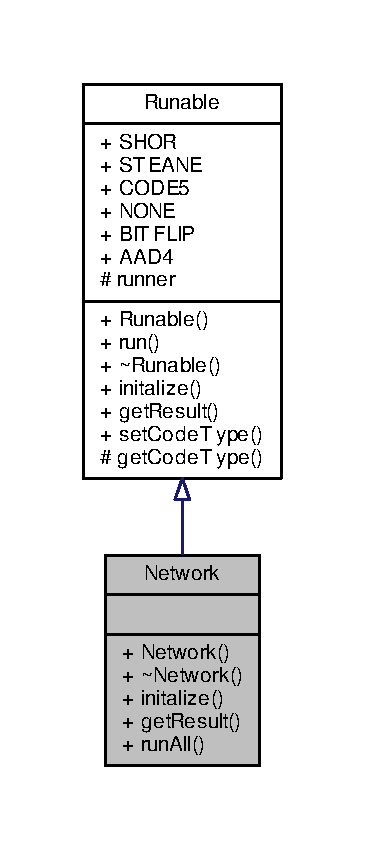
\includegraphics[width=175pt]{class_network__inherit__graph}
\end{center}
\end{figure}
\subsection*{Public Member Functions}
\begin{DoxyCompactItemize}
\item 
\hyperlink{class_network_a7d15ac5c7574b7cf8184e9efd2f5af22}{Network} (int type, unsigned maxnumthreads, std\+::string filename, int n, std\+::string x, bool p)
\item 
virtual \hyperlink{class_network_a7a4e19cdb4bf0c7ecf82baa643831492}{$\sim$\+Network} ()
\item 
void \hyperlink{class_network_aac12b9028bdef1c44984b1c8e111e69d}{initalize} () override
\item 
std\+::string \hyperlink{class_network_a8bd2e1e2117b07661a149b7e6debb99d}{get\+Result} () override
\item 
void \hyperlink{class_network_a10a99f08c6d2f7f019c83b0899a0c56c}{run\+All} ()
\end{DoxyCompactItemize}
\subsection*{Additional Inherited Members}


\subsection{Detailed Description}
Provides parser and \hyperlink{class_runner}{Runner} for network mode 

\subsection{Constructor \& Destructor Documentation}
\index{Network@{Network}!Network@{Network}}
\index{Network@{Network}!Network@{Network}}
\subsubsection[{\texorpdfstring{Network(int type, unsigned maxnumthreads, std\+::string filename, int n, std\+::string x, bool p)}{Network(int type, unsigned maxnumthreads, std::string filename, int n, std::string x, bool p)}}]{\setlength{\rightskip}{0pt plus 5cm}Network\+::\+Network (
\begin{DoxyParamCaption}
\item[{int}]{type, }
\item[{unsigned}]{maxnumthreads, }
\item[{std\+::string}]{filename, }
\item[{int}]{n, }
\item[{std\+::string}]{x, }
\item[{bool}]{p}
\end{DoxyParamCaption}
)\hspace{0.3cm}{\ttfamily [inline]}}\hypertarget{class_network_a7d15ac5c7574b7cf8184e9efd2f5af22}{}\label{class_network_a7d15ac5c7574b7cf8184e9efd2f5af22}
Constructor 
\begin{DoxyParams}{Parameters}
{\em type} & \hyperlink{class_code}{Code} type \\
\hline
{\em maxnumthreads} & Maximum number of threads running \\
\hline
{\em filename} & Input file name \\
\hline
{\em n} & Number of times to run one transmission \\
\hline
\end{DoxyParams}
\index{Network@{Network}!````~Network@{$\sim$\+Network}}
\index{````~Network@{$\sim$\+Network}!Network@{Network}}
\subsubsection[{\texorpdfstring{$\sim$\+Network()}{~Network()}}]{\setlength{\rightskip}{0pt plus 5cm}Network\+::$\sim$\+Network (
\begin{DoxyParamCaption}
{}
\end{DoxyParamCaption}
)\hspace{0.3cm}{\ttfamily [virtual]}}\hypertarget{class_network_a7a4e19cdb4bf0c7ecf82baa643831492}{}\label{class_network_a7a4e19cdb4bf0c7ecf82baa643831492}


\subsection{Member Function Documentation}
\index{Network@{Network}!get\+Result@{get\+Result}}
\index{get\+Result@{get\+Result}!Network@{Network}}
\subsubsection[{\texorpdfstring{get\+Result() override}{getResult() override}}]{\setlength{\rightskip}{0pt plus 5cm}string Network\+::get\+Result (
\begin{DoxyParamCaption}
{}
\end{DoxyParamCaption}
)\hspace{0.3cm}{\ttfamily [override]}, {\ttfamily [virtual]}}\hypertarget{class_network_a8bd2e1e2117b07661a149b7e6debb99d}{}\label{class_network_a8bd2e1e2117b07661a149b7e6debb99d}
Returns result string for one transmission \begin{DoxyReturn}{Returns}
Descriptor string 
\end{DoxyReturn}


Implements \hyperlink{class_runable_a761a0c657253223f3dd7cf2c0762c34e}{Runable}.

\index{Network@{Network}!initalize@{initalize}}
\index{initalize@{initalize}!Network@{Network}}
\subsubsection[{\texorpdfstring{initalize() override}{initalize() override}}]{\setlength{\rightskip}{0pt plus 5cm}void Network\+::initalize (
\begin{DoxyParamCaption}
{}
\end{DoxyParamCaption}
)\hspace{0.3cm}{\ttfamily [override]}, {\ttfamily [virtual]}}\hypertarget{class_network_aac12b9028bdef1c44984b1c8e111e69d}{}\label{class_network_aac12b9028bdef1c44984b1c8e111e69d}
Initalizes \hyperlink{class_runner}{Runner}, using get \hyperlink{class_channel}{Channel} for one pair. {\bfseries current\+Pair must be set before!} 

Implements \hyperlink{class_runable_ae45ce89bb273ba5863e8ca0951caef85}{Runable}.

\index{Network@{Network}!run\+All@{run\+All}}
\index{run\+All@{run\+All}!Network@{Network}}
\subsubsection[{\texorpdfstring{run\+All()}{runAll()}}]{\setlength{\rightskip}{0pt plus 5cm}void Network\+::run\+All (
\begin{DoxyParamCaption}
{}
\end{DoxyParamCaption}
)}\hypertarget{class_network_a10a99f08c6d2f7f019c83b0899a0c56c}{}\label{class_network_a10a99f08c6d2f7f019c83b0899a0c56c}
Runs simulation for each pair of nodes 

The documentation for this class was generated from the following files\+:\begin{DoxyCompactItemize}
\item 
/home/attila/src/qecc-\/netbeans/qecc/\hyperlink{_network_8h}{Network.\+h}\item 
/home/attila/src/qecc-\/netbeans/qecc/\hyperlink{_network_8cpp}{Network.\+cpp}\end{DoxyCompactItemize}

\hypertarget{class_node}{}\section{Node Class Reference}
\label{class_node}\index{Node@{Node}}


{\ttfamily \#include $<$Node.\+h$>$}

\subsection*{Public Member Functions}
\begin{DoxyCompactItemize}
\item 
\hyperlink{class_node_a0f9959ba888e7c36644daab9b2e0e231}{Node} (std\+::string n)
\item 
int \hyperlink{class_node_a3c7b8ccf4dab44216b997c5f63f11d9f}{get\+Id} ()
\item 
std\+::string \hyperlink{class_node_a3e5ac6b5881a3a9d82f3112953c1e546}{get\+Name} ()
\item 
void \hyperlink{class_node_a45c07091d9faf5e5bcc1c0d5223c5aa3}{make\+Dummy} ()
\item 
bool \hyperlink{class_node_a511c13bcb8668db947cdab9b8ef04fe0}{is\+Dummy} ()
\end{DoxyCompactItemize}


\subsection{Detailed Description}
Assigns a unique id to a name 

\subsection{Constructor \& Destructor Documentation}
\index{Node@{Node}!Node@{Node}}
\index{Node@{Node}!Node@{Node}}
\subsubsection[{\texorpdfstring{Node(std\+::string n)}{Node(std::string n)}}]{\setlength{\rightskip}{0pt plus 5cm}Node\+::\+Node (
\begin{DoxyParamCaption}
\item[{std\+::string}]{n}
\end{DoxyParamCaption}
)\hspace{0.3cm}{\ttfamily [inline]}}\hypertarget{class_node_a0f9959ba888e7c36644daab9b2e0e231}{}\label{class_node_a0f9959ba888e7c36644daab9b2e0e231}
Constructor 
\begin{DoxyParams}{Parameters}
{\em n} & Name of the node \\
\hline
\end{DoxyParams}


\subsection{Member Function Documentation}
\index{Node@{Node}!get\+Id@{get\+Id}}
\index{get\+Id@{get\+Id}!Node@{Node}}
\subsubsection[{\texorpdfstring{get\+Id()}{getId()}}]{\setlength{\rightskip}{0pt plus 5cm}int Node\+::get\+Id (
\begin{DoxyParamCaption}
{}
\end{DoxyParamCaption}
)\hspace{0.3cm}{\ttfamily [inline]}}\hypertarget{class_node_a3c7b8ccf4dab44216b997c5f63f11d9f}{}\label{class_node_a3c7b8ccf4dab44216b997c5f63f11d9f}
Returns Id \begin{DoxyReturn}{Returns}
id 
\end{DoxyReturn}
\index{Node@{Node}!get\+Name@{get\+Name}}
\index{get\+Name@{get\+Name}!Node@{Node}}
\subsubsection[{\texorpdfstring{get\+Name()}{getName()}}]{\setlength{\rightskip}{0pt plus 5cm}std\+::string Node\+::get\+Name (
\begin{DoxyParamCaption}
{}
\end{DoxyParamCaption}
)\hspace{0.3cm}{\ttfamily [inline]}}\hypertarget{class_node_a3e5ac6b5881a3a9d82f3112953c1e546}{}\label{class_node_a3e5ac6b5881a3a9d82f3112953c1e546}
Return name \begin{DoxyReturn}{Returns}
name 
\end{DoxyReturn}
\index{Node@{Node}!is\+Dummy@{is\+Dummy}}
\index{is\+Dummy@{is\+Dummy}!Node@{Node}}
\subsubsection[{\texorpdfstring{is\+Dummy()}{isDummy()}}]{\setlength{\rightskip}{0pt plus 5cm}bool Node\+::is\+Dummy (
\begin{DoxyParamCaption}
{}
\end{DoxyParamCaption}
)\hspace{0.3cm}{\ttfamily [inline]}}\hypertarget{class_node_a511c13bcb8668db947cdab9b8ef04fe0}{}\label{class_node_a511c13bcb8668db947cdab9b8ef04fe0}
Returns true if this is a dummy node \index{Node@{Node}!make\+Dummy@{make\+Dummy}}
\index{make\+Dummy@{make\+Dummy}!Node@{Node}}
\subsubsection[{\texorpdfstring{make\+Dummy()}{makeDummy()}}]{\setlength{\rightskip}{0pt plus 5cm}void Node\+::make\+Dummy (
\begin{DoxyParamCaption}
{}
\end{DoxyParamCaption}
)\hspace{0.3cm}{\ttfamily [inline]}}\hypertarget{class_node_a45c07091d9faf5e5bcc1c0d5223c5aa3}{}\label{class_node_a45c07091d9faf5e5bcc1c0d5223c5aa3}
Makes this node a dummy node 

The documentation for this class was generated from the following files\+:\begin{DoxyCompactItemize}
\item 
/home/attila/src/qecc-\/netbeans/qecc/\hyperlink{_node_8h}{Node.\+h}\item 
/home/attila/src/qecc-\/netbeans/qecc/\hyperlink{_node_8cpp}{Node.\+cpp}\end{DoxyCompactItemize}

\hypertarget{class_none}{}\section{None Class Reference}
\label{class_none}\index{None@{None}}


{\ttfamily \#include $<$None.\+h$>$}



Inheritance diagram for None\+:\nopagebreak
\begin{figure}[H]
\begin{center}
\leavevmode
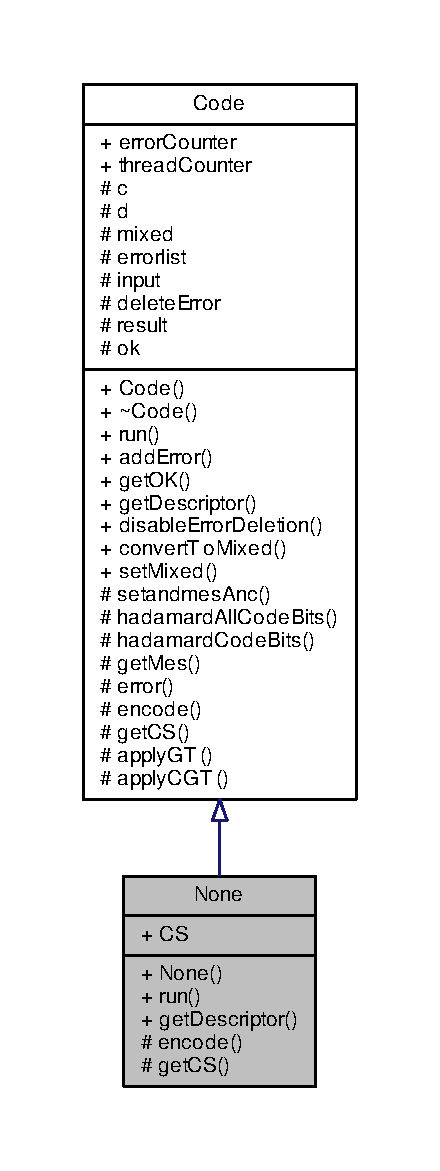
\includegraphics[height=550pt]{class_none__inherit__graph}
\end{center}
\end{figure}
\subsection*{Public Member Functions}
\begin{DoxyCompactItemize}
\item 
\hyperlink{class_none_a57e854dd2b23d85d5476402f85b47ea0}{None} (bool b)
\item 
bool \hyperlink{class_none_aa8386e7d54637a7fd089bb84b5518c9d}{run} () override
\item 
std\+::string \hyperlink{class_none_a0ad5c4d177835a8fc0498d606fefbd79}{get\+Descriptor} () override
\end{DoxyCompactItemize}
\subsection*{Static Public Attributes}
\begin{DoxyCompactItemize}
\item 
static const unsigned \hyperlink{class_none_a7fdf95a5c18d00cc4e81e30f5b04a784}{CS} = 1
\end{DoxyCompactItemize}
\subsection*{Protected Member Functions}
\begin{DoxyCompactItemize}
\item 
void \hyperlink{class_none_a5f7b2a6913822dff79ce6d90b7428ecc}{encode} (bool b) override
\item 
unsigned \hyperlink{class_none_a6e8b66f3489dbc5e1b231c27534c484d}{get\+CS} () override
\end{DoxyCompactItemize}
\subsection*{Additional Inherited Members}


\subsection{Detailed Description}
\hyperlink{class_code}{Code} class using no coding 

\subsection{Constructor \& Destructor Documentation}
\index{None@{None}!None@{None}}
\index{None@{None}!None@{None}}
\subsubsection[{\texorpdfstring{None(bool b)}{None(bool b)}}]{\setlength{\rightskip}{0pt plus 5cm}None\+::\+None (
\begin{DoxyParamCaption}
\item[{bool}]{b}
\end{DoxyParamCaption}
)\hspace{0.3cm}{\ttfamily [inline]}}\hypertarget{class_none_a57e854dd2b23d85d5476402f85b47ea0}{}\label{class_none_a57e854dd2b23d85d5476402f85b47ea0}


\subsection{Member Function Documentation}
\index{None@{None}!encode@{encode}}
\index{encode@{encode}!None@{None}}
\subsubsection[{\texorpdfstring{encode(bool b) override}{encode(bool b) override}}]{\setlength{\rightskip}{0pt plus 5cm}void None\+::encode (
\begin{DoxyParamCaption}
\item[{bool}]{b}
\end{DoxyParamCaption}
)\hspace{0.3cm}{\ttfamily [override]}, {\ttfamily [protected]}, {\ttfamily [virtual]}}\hypertarget{class_none_a5f7b2a6913822dff79ce6d90b7428ecc}{}\label{class_none_a5f7b2a6913822dff79ce6d90b7428ecc}
Encode input bit 
\begin{DoxyParams}{Parameters}
{\em b} & Classical input converted to $\vert$0$>$ or $\vert$1$>$ \\
\hline
\end{DoxyParams}


Implements \hyperlink{class_code_a5f90b0f96002c9b999d8ed7bab319906}{Code}.

\index{None@{None}!get\+CS@{get\+CS}}
\index{get\+CS@{get\+CS}!None@{None}}
\subsubsection[{\texorpdfstring{get\+C\+S() override}{getCS() override}}]{\setlength{\rightskip}{0pt plus 5cm}unsigned None\+::get\+CS (
\begin{DoxyParamCaption}
{}
\end{DoxyParamCaption}
)\hspace{0.3cm}{\ttfamily [inline]}, {\ttfamily [override]}, {\ttfamily [protected]}, {\ttfamily [virtual]}}\hypertarget{class_none_a6e8b66f3489dbc5e1b231c27534c484d}{}\label{class_none_a6e8b66f3489dbc5e1b231c27534c484d}
Return code size of a child \begin{DoxyReturn}{Returns}
code size 
\end{DoxyReturn}


Implements \hyperlink{class_code_a34f52b25d78aeaec3c1fd381f025ad00}{Code}.

\index{None@{None}!get\+Descriptor@{get\+Descriptor}}
\index{get\+Descriptor@{get\+Descriptor}!None@{None}}
\subsubsection[{\texorpdfstring{get\+Descriptor() override}{getDescriptor() override}}]{\setlength{\rightskip}{0pt plus 5cm}std\+::string None\+::get\+Descriptor (
\begin{DoxyParamCaption}
{}
\end{DoxyParamCaption}
)\hspace{0.3cm}{\ttfamily [override]}, {\ttfamily [virtual]}}\hypertarget{class_none_a0ad5c4d177835a8fc0498d606fefbd79}{}\label{class_none_a0ad5c4d177835a8fc0498d606fefbd79}
Returns a descriptor string~\newline
 Format\+:~\newline
 {\itshape N\+O\+NE i-\/$>$o E\+R\+R\+O\+R/\+OK} \begin{DoxyReturn}{Returns}
Log string 
\end{DoxyReturn}


Implements \hyperlink{class_code_a60db2f615a7cff76e3ece1c486b2fd16}{Code}.

\index{None@{None}!run@{run}}
\index{run@{run}!None@{None}}
\subsubsection[{\texorpdfstring{run() override}{run() override}}]{\setlength{\rightskip}{0pt plus 5cm}bool None\+::run (
\begin{DoxyParamCaption}
{}
\end{DoxyParamCaption}
)\hspace{0.3cm}{\ttfamily [override]}, {\ttfamily [virtual]}}\hypertarget{class_none_aa8386e7d54637a7fd089bb84b5518c9d}{}\label{class_none_aa8386e7d54637a7fd089bb84b5518c9d}
Function to simulate the transmission and get the result. To be defined in child classes. \begin{DoxyReturn}{Returns}
Measured bit at Bob 
\end{DoxyReturn}


Implements \hyperlink{class_code_a5621bbd050948ba1e41f69f451a05990}{Code}.



\subsection{Member Data Documentation}
\index{None@{None}!CS@{CS}}
\index{CS@{CS}!None@{None}}
\subsubsection[{\texorpdfstring{CS}{CS}}]{\setlength{\rightskip}{0pt plus 5cm}const unsigned None\+::\+CS = 1\hspace{0.3cm}{\ttfamily [static]}}\hypertarget{class_none_a7fdf95a5c18d00cc4e81e30f5b04a784}{}\label{class_none_a7fdf95a5c18d00cc4e81e30f5b04a784}
\hyperlink{class_code}{Code} size for \hyperlink{class_none}{None} is 1 

The documentation for this class was generated from the following files\+:\begin{DoxyCompactItemize}
\item 
/home/attila/src/qecc-\/netbeans/qecc/\hyperlink{_none_8h}{None.\+h}\item 
/home/attila/src/qecc-\/netbeans/qecc/\hyperlink{_none_8cpp}{None.\+cpp}\end{DoxyCompactItemize}

\hypertarget{class_runable}{}\section{Runable Class Reference}
\label{class_runable}\index{Runable@{Runable}}


{\ttfamily \#include $<$Runable.\+h$>$}



Inheritance diagram for Runable\+:\nopagebreak
\begin{figure}[H]
\begin{center}
\leavevmode
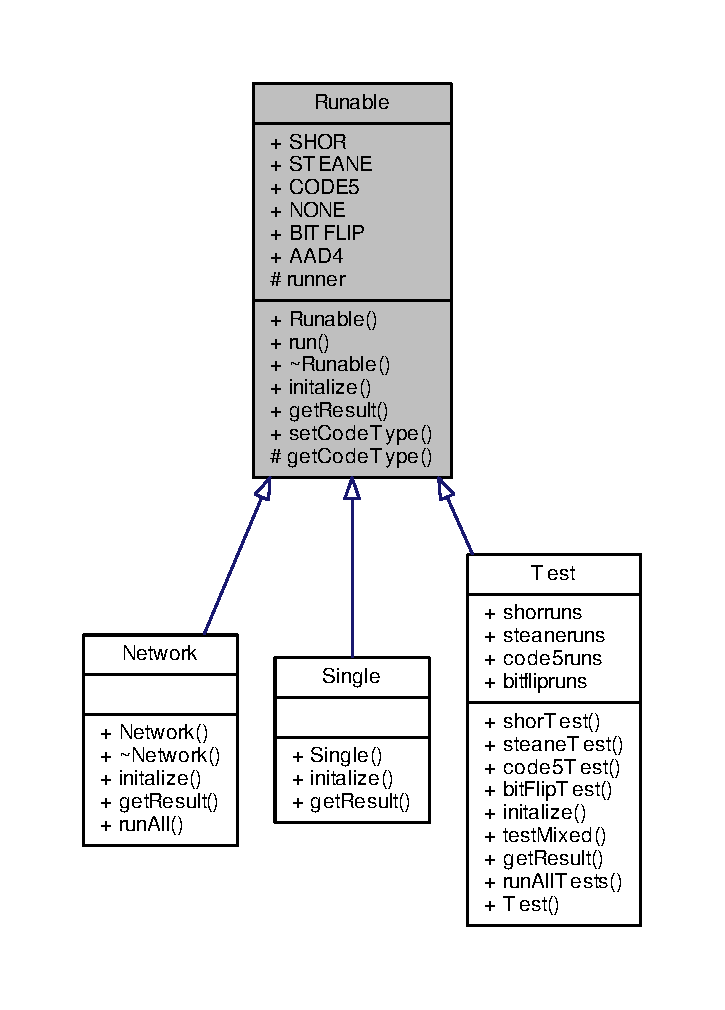
\includegraphics[width=348pt]{class_runable__inherit__graph}
\end{center}
\end{figure}
\subsection*{Public Member Functions}
\begin{DoxyCompactItemize}
\item 
\hyperlink{class_runable_a3e264e6a6e374f7111d5c4fea0a6ca3c}{Runable} (int type, unsigned maxnumthreads, bool p)
\item 
void \hyperlink{class_runable_a766cbda482eeb5c181941f1a1113041c}{run} ()
\item 
virtual \hyperlink{class_runable_a6b1e67cab0fb137e26963f6e8d2687d4}{$\sim$\+Runable} ()
\item 
virtual void \hyperlink{class_runable_ae45ce89bb273ba5863e8ca0951caef85}{initalize} ()=0
\item 
virtual std\+::string \hyperlink{class_runable_a761a0c657253223f3dd7cf2c0762c34e}{get\+Result} ()=0
\item 
void \hyperlink{class_runable_a41f4c8d84fa427f05b82bb530d19e454}{set\+Code\+Type} (int t)
\end{DoxyCompactItemize}
\subsection*{Static Public Attributes}
\begin{DoxyCompactItemize}
\item 
static const int \hyperlink{class_runable_a27f57a3218c5237bdd5c0134db82e3f9}{S\+H\+OR} = 100
\item 
static const int \hyperlink{class_runable_a68af748dc3edebef5e1dd7a3e18a1b5f}{S\+T\+E\+A\+NE} = 101
\item 
static const int \hyperlink{class_runable_ad3dbc64c086f9e02f45c8e877f5ae898}{C\+O\+D\+E5} = 102
\item 
static const int \hyperlink{class_runable_a9dfae104f3c3623e9e39908c1560a7fe}{N\+O\+NE} = 103
\item 
static const int \hyperlink{class_runable_a56fc454699fbd4fcbe05bb90c36b80b0}{B\+I\+T\+F\+L\+IP} = 104
\item 
static const int \hyperlink{class_runable_a89b302b9a67e49ca32abd77560b58bdb}{A\+A\+D4} = 105
\end{DoxyCompactItemize}
\subsection*{Protected Member Functions}
\begin{DoxyCompactItemize}
\item 
int \hyperlink{class_runable_a9e9e55d77ae3cf5486fc60bae62f1141}{get\+Code\+Type} ()
\end{DoxyCompactItemize}
\subsection*{Protected Attributes}
\begin{DoxyCompactItemize}
\item 
\hyperlink{class_runner}{Runner} $\ast$ \hyperlink{class_runable_ad61073e4e8d33b564701edd7e30a967f}{runner}
\end{DoxyCompactItemize}


\subsection{Detailed Description}
\hyperlink{class_runable}{Runable} provides container for \hyperlink{class_runner}{Runner} 

\subsection{Constructor \& Destructor Documentation}
\index{Runable@{Runable}!Runable@{Runable}}
\index{Runable@{Runable}!Runable@{Runable}}
\subsubsection[{\texorpdfstring{Runable(int type, unsigned maxnumthreads, bool p)}{Runable(int type, unsigned maxnumthreads, bool p)}}]{\setlength{\rightskip}{0pt plus 5cm}Runable\+::\+Runable (
\begin{DoxyParamCaption}
\item[{int}]{type, }
\item[{unsigned}]{maxnumthreads, }
\item[{bool}]{p}
\end{DoxyParamCaption}
)\hspace{0.3cm}{\ttfamily [inline]}}\hypertarget{class_runable_a3e264e6a6e374f7111d5c4fea0a6ca3c}{}\label{class_runable_a3e264e6a6e374f7111d5c4fea0a6ca3c}
Constructor 
\begin{DoxyParams}{Parameters}
{\em type} & \hyperlink{class_code}{Code} type \\
\hline
{\em maxnumthreads} & Maximum number of threads running \\
\hline
\end{DoxyParams}
\index{Runable@{Runable}!````~Runable@{$\sim$\+Runable}}
\index{````~Runable@{$\sim$\+Runable}!Runable@{Runable}}
\subsubsection[{\texorpdfstring{$\sim$\+Runable()}{~Runable()}}]{\setlength{\rightskip}{0pt plus 5cm}Runable\+::$\sim$\+Runable (
\begin{DoxyParamCaption}
{}
\end{DoxyParamCaption}
)\hspace{0.3cm}{\ttfamily [virtual]}}\hypertarget{class_runable_a6b1e67cab0fb137e26963f6e8d2687d4}{}\label{class_runable_a6b1e67cab0fb137e26963f6e8d2687d4}


\subsection{Member Function Documentation}
\index{Runable@{Runable}!get\+Code\+Type@{get\+Code\+Type}}
\index{get\+Code\+Type@{get\+Code\+Type}!Runable@{Runable}}
\subsubsection[{\texorpdfstring{get\+Code\+Type()}{getCodeType()}}]{\setlength{\rightskip}{0pt plus 5cm}int Runable\+::get\+Code\+Type (
\begin{DoxyParamCaption}
{}
\end{DoxyParamCaption}
)\hspace{0.3cm}{\ttfamily [inline]}, {\ttfamily [protected]}}\hypertarget{class_runable_a9e9e55d77ae3cf5486fc60bae62f1141}{}\label{class_runable_a9e9e55d77ae3cf5486fc60bae62f1141}
\begin{DoxyReturn}{Returns}
code type 
\end{DoxyReturn}
\index{Runable@{Runable}!get\+Result@{get\+Result}}
\index{get\+Result@{get\+Result}!Runable@{Runable}}
\subsubsection[{\texorpdfstring{get\+Result()=0}{getResult()=0}}]{\setlength{\rightskip}{0pt plus 5cm}virtual std\+::string Runable\+::get\+Result (
\begin{DoxyParamCaption}
{}
\end{DoxyParamCaption}
)\hspace{0.3cm}{\ttfamily [pure virtual]}}\hypertarget{class_runable_a761a0c657253223f3dd7cf2c0762c34e}{}\label{class_runable_a761a0c657253223f3dd7cf2c0762c34e}
Returns descriptor string. To be defined by child! \begin{DoxyReturn}{Returns}
Log string 
\end{DoxyReturn}


Implemented in \hyperlink{class_test_ae53178c2e482ed3a869c742387521a60}{Test}, \hyperlink{class_network_a8bd2e1e2117b07661a149b7e6debb99d}{Network}, and \hyperlink{class_single_adcafbbcea43758d47c2f8b4e0704c8dd}{Single}.

\index{Runable@{Runable}!initalize@{initalize}}
\index{initalize@{initalize}!Runable@{Runable}}
\subsubsection[{\texorpdfstring{initalize()=0}{initalize()=0}}]{\setlength{\rightskip}{0pt plus 5cm}virtual void Runable\+::initalize (
\begin{DoxyParamCaption}
{}
\end{DoxyParamCaption}
)\hspace{0.3cm}{\ttfamily [pure virtual]}}\hypertarget{class_runable_ae45ce89bb273ba5863e8ca0951caef85}{}\label{class_runable_ae45ce89bb273ba5863e8ca0951caef85}
Initalizes code list. To be defined by child! 

Implemented in \hyperlink{class_test_a6baf4b2ddf84f198e156bf78c97b865b}{Test}, \hyperlink{class_network_aac12b9028bdef1c44984b1c8e111e69d}{Network}, and \hyperlink{class_single_afa7dc40314a46c75553a1de77ce020e9}{Single}.

\index{Runable@{Runable}!run@{run}}
\index{run@{run}!Runable@{Runable}}
\subsubsection[{\texorpdfstring{run()}{run()}}]{\setlength{\rightskip}{0pt plus 5cm}void Runable\+::run (
\begin{DoxyParamCaption}
{}
\end{DoxyParamCaption}
)\hspace{0.3cm}{\ttfamily [inline]}}\hypertarget{class_runable_a766cbda482eeb5c181941f1a1113041c}{}\label{class_runable_a766cbda482eeb5c181941f1a1113041c}
Runs codes \index{Runable@{Runable}!set\+Code\+Type@{set\+Code\+Type}}
\index{set\+Code\+Type@{set\+Code\+Type}!Runable@{Runable}}
\subsubsection[{\texorpdfstring{set\+Code\+Type(int t)}{setCodeType(int t)}}]{\setlength{\rightskip}{0pt plus 5cm}void Runable\+::set\+Code\+Type (
\begin{DoxyParamCaption}
\item[{int}]{t}
\end{DoxyParamCaption}
)\hspace{0.3cm}{\ttfamily [inline]}}\hypertarget{class_runable_a41f4c8d84fa427f05b82bb530d19e454}{}\label{class_runable_a41f4c8d84fa427f05b82bb530d19e454}
Sets code type to another 
\begin{DoxyParams}{Parameters}
{\em t} & code type \\
\hline
\end{DoxyParams}


\subsection{Member Data Documentation}
\index{Runable@{Runable}!A\+A\+D4@{A\+A\+D4}}
\index{A\+A\+D4@{A\+A\+D4}!Runable@{Runable}}
\subsubsection[{\texorpdfstring{A\+A\+D4}{AAD4}}]{\setlength{\rightskip}{0pt plus 5cm}const int Runable\+::\+A\+A\+D4 = 105\hspace{0.3cm}{\ttfamily [static]}}\hypertarget{class_runable_a89b302b9a67e49ca32abd77560b58bdb}{}\label{class_runable_a89b302b9a67e49ca32abd77560b58bdb}
4qubit amplitude damping code type int \index{Runable@{Runable}!B\+I\+T\+F\+L\+IP@{B\+I\+T\+F\+L\+IP}}
\index{B\+I\+T\+F\+L\+IP@{B\+I\+T\+F\+L\+IP}!Runable@{Runable}}
\subsubsection[{\texorpdfstring{B\+I\+T\+F\+L\+IP}{BITFLIP}}]{\setlength{\rightskip}{0pt plus 5cm}const int Runable\+::\+B\+I\+T\+F\+L\+IP = 104\hspace{0.3cm}{\ttfamily [static]}}\hypertarget{class_runable_a56fc454699fbd4fcbe05bb90c36b80b0}{}\label{class_runable_a56fc454699fbd4fcbe05bb90c36b80b0}
Bit flip code type int \index{Runable@{Runable}!C\+O\+D\+E5@{C\+O\+D\+E5}}
\index{C\+O\+D\+E5@{C\+O\+D\+E5}!Runable@{Runable}}
\subsubsection[{\texorpdfstring{C\+O\+D\+E5}{CODE5}}]{\setlength{\rightskip}{0pt plus 5cm}const int Runable\+::\+C\+O\+D\+E5 = 102\hspace{0.3cm}{\ttfamily [static]}}\hypertarget{class_runable_ad3dbc64c086f9e02f45c8e877f5ae898}{}\label{class_runable_ad3dbc64c086f9e02f45c8e877f5ae898}
5qubit code type int \index{Runable@{Runable}!N\+O\+NE@{N\+O\+NE}}
\index{N\+O\+NE@{N\+O\+NE}!Runable@{Runable}}
\subsubsection[{\texorpdfstring{N\+O\+NE}{NONE}}]{\setlength{\rightskip}{0pt plus 5cm}const int Runable\+::\+N\+O\+NE = 103\hspace{0.3cm}{\ttfamily [static]}}\hypertarget{class_runable_a9dfae104f3c3623e9e39908c1560a7fe}{}\label{class_runable_a9dfae104f3c3623e9e39908c1560a7fe}
No coding type int \index{Runable@{Runable}!runner@{runner}}
\index{runner@{runner}!Runable@{Runable}}
\subsubsection[{\texorpdfstring{runner}{runner}}]{\setlength{\rightskip}{0pt plus 5cm}{\bf Runner}$\ast$ Runable\+::runner\hspace{0.3cm}{\ttfamily [protected]}}\hypertarget{class_runable_ad61073e4e8d33b564701edd7e30a967f}{}\label{class_runable_ad61073e4e8d33b564701edd7e30a967f}
\hyperlink{class_runner}{Runner} to provide multithreading \index{Runable@{Runable}!S\+H\+OR@{S\+H\+OR}}
\index{S\+H\+OR@{S\+H\+OR}!Runable@{Runable}}
\subsubsection[{\texorpdfstring{S\+H\+OR}{SHOR}}]{\setlength{\rightskip}{0pt plus 5cm}const int Runable\+::\+S\+H\+OR = 100\hspace{0.3cm}{\ttfamily [static]}}\hypertarget{class_runable_a27f57a3218c5237bdd5c0134db82e3f9}{}\label{class_runable_a27f57a3218c5237bdd5c0134db82e3f9}
\hyperlink{class_shor}{Shor} code type int \index{Runable@{Runable}!S\+T\+E\+A\+NE@{S\+T\+E\+A\+NE}}
\index{S\+T\+E\+A\+NE@{S\+T\+E\+A\+NE}!Runable@{Runable}}
\subsubsection[{\texorpdfstring{S\+T\+E\+A\+NE}{STEANE}}]{\setlength{\rightskip}{0pt plus 5cm}const int Runable\+::\+S\+T\+E\+A\+NE = 101\hspace{0.3cm}{\ttfamily [static]}}\hypertarget{class_runable_a68af748dc3edebef5e1dd7a3e18a1b5f}{}\label{class_runable_a68af748dc3edebef5e1dd7a3e18a1b5f}
\hyperlink{class_steane}{Steane} code type int 

The documentation for this class was generated from the following files\+:\begin{DoxyCompactItemize}
\item 
/home/attila/src/qecc-\/netbeans/qecc/\hyperlink{_runable_8h}{Runable.\+h}\item 
/home/attila/src/qecc-\/netbeans/qecc/\hyperlink{_runable_8cpp}{Runable.\+cpp}\end{DoxyCompactItemize}

\hypertarget{class_runner}{}\section{Runner Class Reference}
\label{class_runner}\index{Runner@{Runner}}


{\ttfamily \#include $<$Runner.\+h$>$}

\subsection*{Public Member Functions}
\begin{DoxyCompactItemize}
\item 
\hyperlink{class_runner_a6fff7359862c9eb1e0ab566efa572cd2}{Runner} (unsigned maxnumthreads)
\item 
virtual \hyperlink{class_runner_aec894ad000798237c0975d1ef198522b}{$\sim$\+Runner} ()
\item 
void \hyperlink{class_runner_a1901d1762c18b824e8cf76042816a24b}{add\+Code} (\hyperlink{class_code}{Code} $\ast$c)
\item 
void \hyperlink{class_runner_a352a9423f54145f34abec68a1570b653}{run} ()
\item 
void \hyperlink{class_runner_ac004bc561dd4e784e4142fb7bd331e0f}{reset} ()
\item 
float \hyperlink{class_runner_a21528c823de77ee5947b6e38d634fdf5}{get\+B\+ER} ()
\item 
void \hyperlink{class_runner_a4dce4c81aa544ff23066965b804c1f45}{plus\+Minus} ()
\end{DoxyCompactItemize}


\subsection{Detailed Description}
Runs codes multithreaded 

\subsection{Constructor \& Destructor Documentation}
\index{Runner@{Runner}!Runner@{Runner}}
\index{Runner@{Runner}!Runner@{Runner}}
\subsubsection[{\texorpdfstring{Runner(unsigned maxnumthreads)}{Runner(unsigned maxnumthreads)}}]{\setlength{\rightskip}{0pt plus 5cm}Runner\+::\+Runner (
\begin{DoxyParamCaption}
\item[{unsigned}]{maxnumthreads}
\end{DoxyParamCaption}
)}\hypertarget{class_runner_a6fff7359862c9eb1e0ab566efa572cd2}{}\label{class_runner_a6fff7359862c9eb1e0ab566efa572cd2}
Constructor 
\begin{DoxyParams}{Parameters}
{\em maxnumthreads} & Maximum number of thread running \\
\hline
\end{DoxyParams}
\index{Runner@{Runner}!````~Runner@{$\sim$\+Runner}}
\index{````~Runner@{$\sim$\+Runner}!Runner@{Runner}}
\subsubsection[{\texorpdfstring{$\sim$\+Runner()}{~Runner()}}]{\setlength{\rightskip}{0pt plus 5cm}Runner\+::$\sim$\+Runner (
\begin{DoxyParamCaption}
{}
\end{DoxyParamCaption}
)\hspace{0.3cm}{\ttfamily [virtual]}}\hypertarget{class_runner_aec894ad000798237c0975d1ef198522b}{}\label{class_runner_aec894ad000798237c0975d1ef198522b}


\subsection{Member Function Documentation}
\index{Runner@{Runner}!add\+Code@{add\+Code}}
\index{add\+Code@{add\+Code}!Runner@{Runner}}
\subsubsection[{\texorpdfstring{add\+Code(\+Code $\ast$c)}{addCode(Code *c)}}]{\setlength{\rightskip}{0pt plus 5cm}void Runner\+::add\+Code (
\begin{DoxyParamCaption}
\item[{{\bf Code} $\ast$}]{c}
\end{DoxyParamCaption}
)}\hypertarget{class_runner_a1901d1762c18b824e8cf76042816a24b}{}\label{class_runner_a1901d1762c18b824e8cf76042816a24b}
Adds code to code list 
\begin{DoxyParams}{Parameters}
{\em c} & Pointer to the code to be added \\
\hline
\end{DoxyParams}
\index{Runner@{Runner}!get\+B\+ER@{get\+B\+ER}}
\index{get\+B\+ER@{get\+B\+ER}!Runner@{Runner}}
\subsubsection[{\texorpdfstring{get\+B\+E\+R()}{getBER()}}]{\setlength{\rightskip}{0pt plus 5cm}float Runner\+::get\+B\+ER (
\begin{DoxyParamCaption}
{}
\end{DoxyParamCaption}
)\hspace{0.3cm}{\ttfamily [inline]}}\hypertarget{class_runner_a21528c823de77ee5947b6e38d634fdf5}{}\label{class_runner_a21528c823de77ee5947b6e38d634fdf5}
Get bit error rate \begin{DoxyReturn}{Returns}
Bit error rate 
\end{DoxyReturn}
\index{Runner@{Runner}!plus\+Minus@{plus\+Minus}}
\index{plus\+Minus@{plus\+Minus}!Runner@{Runner}}
\subsubsection[{\texorpdfstring{plus\+Minus()}{plusMinus()}}]{\setlength{\rightskip}{0pt plus 5cm}void Runner\+::plus\+Minus (
\begin{DoxyParamCaption}
{}
\end{DoxyParamCaption}
)\hspace{0.3cm}{\ttfamily [inline]}}\hypertarget{class_runner_a4dce4c81aa544ff23066965b804c1f45}{}\label{class_runner_a4dce4c81aa544ff23066965b804c1f45}
Run codes with ket+, ket-\/ inputs \index{Runner@{Runner}!reset@{reset}}
\index{reset@{reset}!Runner@{Runner}}
\subsubsection[{\texorpdfstring{reset()}{reset()}}]{\setlength{\rightskip}{0pt plus 5cm}void Runner\+::reset (
\begin{DoxyParamCaption}
{}
\end{DoxyParamCaption}
)\hspace{0.3cm}{\ttfamily [inline]}}\hypertarget{class_runner_ac004bc561dd4e784e4142fb7bd331e0f}{}\label{class_runner_ac004bc561dd4e784e4142fb7bd331e0f}
Reset status normally run by \hyperlink{class_runner_a352a9423f54145f34abec68a1570b653}{run()} \index{Runner@{Runner}!run@{run}}
\index{run@{run}!Runner@{Runner}}
\subsubsection[{\texorpdfstring{run()}{run()}}]{\setlength{\rightskip}{0pt plus 5cm}void Runner\+::run (
\begin{DoxyParamCaption}
{}
\end{DoxyParamCaption}
)}\hypertarget{class_runner_a352a9423f54145f34abec68a1570b653}{}\label{class_runner_a352a9423f54145f34abec68a1570b653}
Runs codes in code list 

The documentation for this class was generated from the following files\+:\begin{DoxyCompactItemize}
\item 
/home/attila/src/qecc-\/netbeans/qecc/\hyperlink{_runner_8h}{Runner.\+h}\item 
/home/attila/src/qecc-\/netbeans/qecc/\hyperlink{_runner_8cpp}{Runner.\+cpp}\end{DoxyCompactItemize}

\hypertarget{class_shor}{}\section{Shor Class Reference}
\label{class_shor}\index{Shor@{Shor}}


{\ttfamily \#include $<$Shor.\+h$>$}



Inheritance diagram for Shor\+:\nopagebreak
\begin{figure}[H]
\begin{center}
\leavevmode
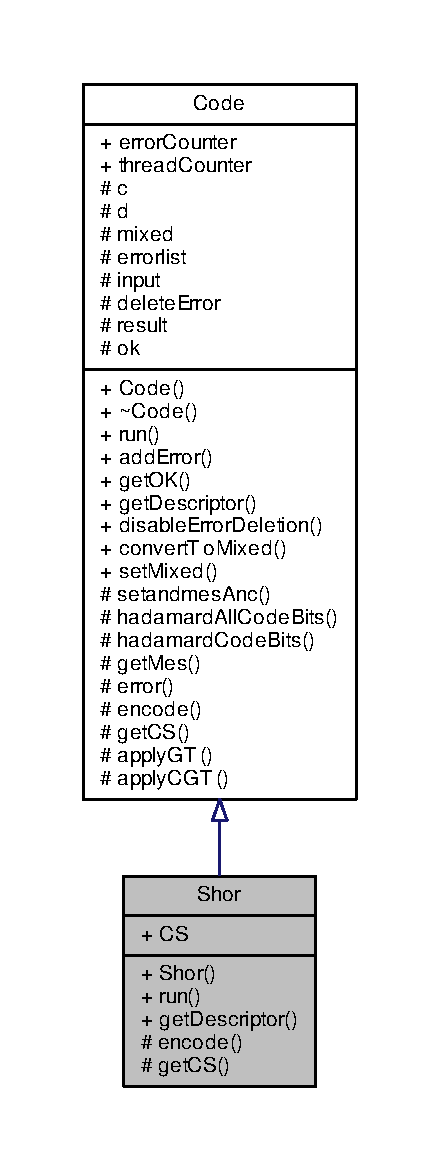
\includegraphics[height=550pt]{class_shor__inherit__graph}
\end{center}
\end{figure}
\subsection*{Public Types}
\begin{DoxyCompactItemize}
\item 
typedef \hyperlink{class_code}{Code} \hyperlink{class_shor_a7ea95c357f9d816b3a37176aa4e01781}{super}
\end{DoxyCompactItemize}
\subsection*{Public Member Functions}
\begin{DoxyCompactItemize}
\item 
\hyperlink{class_shor_ac7cca820563c3eb81c28a8fc736249b6}{Shor} (bool b)
\item 
bool \hyperlink{class_shor_abe454e38fed6f33d832c3d7fd64627ea}{run} () override
\item 
std\+::string \hyperlink{class_shor_ad9a43efd28edf5df378d0c6b7dfbb051}{get\+Descriptor} () override
\end{DoxyCompactItemize}
\subsection*{Static Public Attributes}
\begin{DoxyCompactItemize}
\item 
static const unsigned \hyperlink{class_shor_a5c2bb5ad73004577f8781a001eda8b8f}{CS} = 9
\end{DoxyCompactItemize}
\subsection*{Protected Member Functions}
\begin{DoxyCompactItemize}
\item 
void \hyperlink{class_shor_a77db4d99076a0e581057faae8071574c}{encode} (bool b) override
\item 
unsigned \hyperlink{class_shor_a5cfb32ea0c6f73fd9478ce93b7fafb4f}{get\+CS} () override
\end{DoxyCompactItemize}
\subsection*{Additional Inherited Members}


\subsection{Detailed Description}
\hyperlink{class_shor}{Shor} code class 

\subsection{Member Typedef Documentation}
\index{Shor@{Shor}!super@{super}}
\index{super@{super}!Shor@{Shor}}
\subsubsection[{\texorpdfstring{super}{super}}]{\setlength{\rightskip}{0pt plus 5cm}typedef {\bf Code} {\bf Shor\+::super}}\hypertarget{class_shor_a7ea95c357f9d816b3a37176aa4e01781}{}\label{class_shor_a7ea95c357f9d816b3a37176aa4e01781}


\subsection{Constructor \& Destructor Documentation}
\index{Shor@{Shor}!Shor@{Shor}}
\index{Shor@{Shor}!Shor@{Shor}}
\subsubsection[{\texorpdfstring{Shor(bool b)}{Shor(bool b)}}]{\setlength{\rightskip}{0pt plus 5cm}Shor\+::\+Shor (
\begin{DoxyParamCaption}
\item[{bool}]{b}
\end{DoxyParamCaption}
)\hspace{0.3cm}{\ttfamily [inline]}}\hypertarget{class_shor_ac7cca820563c3eb81c28a8fc736249b6}{}\label{class_shor_ac7cca820563c3eb81c28a8fc736249b6}


\subsection{Member Function Documentation}
\index{Shor@{Shor}!encode@{encode}}
\index{encode@{encode}!Shor@{Shor}}
\subsubsection[{\texorpdfstring{encode(bool b) override}{encode(bool b) override}}]{\setlength{\rightskip}{0pt plus 5cm}void Shor\+::encode (
\begin{DoxyParamCaption}
\item[{bool}]{b}
\end{DoxyParamCaption}
)\hspace{0.3cm}{\ttfamily [override]}, {\ttfamily [protected]}, {\ttfamily [virtual]}}\hypertarget{class_shor_a77db4d99076a0e581057faae8071574c}{}\label{class_shor_a77db4d99076a0e581057faae8071574c}
Encode input bit 
\begin{DoxyParams}{Parameters}
{\em b} & Classical input converted to $\vert$0$>$ or $\vert$1$>$ \\
\hline
\end{DoxyParams}


Implements \hyperlink{class_code_a5f90b0f96002c9b999d8ed7bab319906}{Code}.

\index{Shor@{Shor}!get\+CS@{get\+CS}}
\index{get\+CS@{get\+CS}!Shor@{Shor}}
\subsubsection[{\texorpdfstring{get\+C\+S() override}{getCS() override}}]{\setlength{\rightskip}{0pt plus 5cm}unsigned Shor\+::get\+CS (
\begin{DoxyParamCaption}
{}
\end{DoxyParamCaption}
)\hspace{0.3cm}{\ttfamily [inline]}, {\ttfamily [override]}, {\ttfamily [protected]}, {\ttfamily [virtual]}}\hypertarget{class_shor_a5cfb32ea0c6f73fd9478ce93b7fafb4f}{}\label{class_shor_a5cfb32ea0c6f73fd9478ce93b7fafb4f}
Return code size of a child \begin{DoxyReturn}{Returns}
code size 
\end{DoxyReturn}


Implements \hyperlink{class_code_a34f52b25d78aeaec3c1fd381f025ad00}{Code}.

\index{Shor@{Shor}!get\+Descriptor@{get\+Descriptor}}
\index{get\+Descriptor@{get\+Descriptor}!Shor@{Shor}}
\subsubsection[{\texorpdfstring{get\+Descriptor() override}{getDescriptor() override}}]{\setlength{\rightskip}{0pt plus 5cm}std\+::string Shor\+::get\+Descriptor (
\begin{DoxyParamCaption}
{}
\end{DoxyParamCaption}
)\hspace{0.3cm}{\ttfamily [override]}, {\ttfamily [virtual]}}\hypertarget{class_shor_ad9a43efd28edf5df378d0c6b7dfbb051}{}\label{class_shor_ad9a43efd28edf5df378d0c6b7dfbb051}
Returns descriptor string ~\newline
 Format\+: ~\newline
 {\itshape S\+H\+OR aabbcc zz i-\/$>$o O\+K/\+E\+R\+R\+OR} ~\newline
 Where aabbcc is xflip, zz is zflip \begin{DoxyReturn}{Returns}
Log string 
\end{DoxyReturn}


Implements \hyperlink{class_code_a60db2f615a7cff76e3ece1c486b2fd16}{Code}.

\index{Shor@{Shor}!run@{run}}
\index{run@{run}!Shor@{Shor}}
\subsubsection[{\texorpdfstring{run() override}{run() override}}]{\setlength{\rightskip}{0pt plus 5cm}bool Shor\+::run (
\begin{DoxyParamCaption}
{}
\end{DoxyParamCaption}
)\hspace{0.3cm}{\ttfamily [override]}, {\ttfamily [virtual]}}\hypertarget{class_shor_abe454e38fed6f33d832c3d7fd64627ea}{}\label{class_shor_abe454e38fed6f33d832c3d7fd64627ea}
Function to simulate the transmission and get the result. To be defined in child classes. \begin{DoxyReturn}{Returns}
Measured bit at Bob 
\end{DoxyReturn}


Implements \hyperlink{class_code_a5621bbd050948ba1e41f69f451a05990}{Code}.



\subsection{Member Data Documentation}
\index{Shor@{Shor}!CS@{CS}}
\index{CS@{CS}!Shor@{Shor}}
\subsubsection[{\texorpdfstring{CS}{CS}}]{\setlength{\rightskip}{0pt plus 5cm}const unsigned Shor\+::\+CS = 9\hspace{0.3cm}{\ttfamily [static]}}\hypertarget{class_shor_a5c2bb5ad73004577f8781a001eda8b8f}{}\label{class_shor_a5c2bb5ad73004577f8781a001eda8b8f}
\hyperlink{class_code}{Code} size for \hyperlink{class_shor}{Shor} is 9 

The documentation for this class was generated from the following files\+:\begin{DoxyCompactItemize}
\item 
/home/attila/src/qecc-\/netbeans/qecc/\hyperlink{_shor_8h}{Shor.\+h}\item 
/home/attila/src/qecc-\/netbeans/qecc/\hyperlink{_shor_8cpp}{Shor.\+cpp}\end{DoxyCompactItemize}

\hypertarget{class_single}{}\section{Single Class Reference}
\label{class_single}\index{Single@{Single}}


{\ttfamily \#include $<$Single.\+h$>$}



Inheritance diagram for Single\+:\nopagebreak
\begin{figure}[H]
\begin{center}
\leavevmode
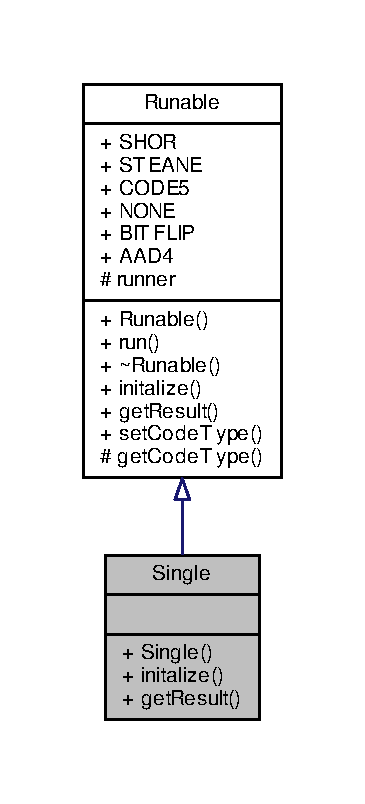
\includegraphics[width=175pt]{class_single__inherit__graph}
\end{center}
\end{figure}
\subsection*{Public Member Functions}
\begin{DoxyCompactItemize}
\item 
\hyperlink{class_single_ac3a75d9c9c94671ba0246b581982db69}{Single} (int type, int maxnumthreads, \hyperlink{class_error}{Error} $\ast$e, int n)
\item 
void \hyperlink{class_single_afa7dc40314a46c75553a1de77ce020e9}{initalize} () override
\item 
std\+::string \hyperlink{class_single_adcafbbcea43758d47c2f8b4e0704c8dd}{get\+Result} () override
\end{DoxyCompactItemize}
\subsection*{Additional Inherited Members}


\subsection{Detailed Description}
\hyperlink{class_single}{Single} class runs a single error channel n times 

\subsection{Constructor \& Destructor Documentation}
\index{Single@{Single}!Single@{Single}}
\index{Single@{Single}!Single@{Single}}
\subsubsection[{\texorpdfstring{Single(int type, int maxnumthreads, Error $\ast$e, int n)}{Single(int type, int maxnumthreads, Error *e, int n)}}]{\setlength{\rightskip}{0pt plus 5cm}Single\+::\+Single (
\begin{DoxyParamCaption}
\item[{int}]{type, }
\item[{int}]{maxnumthreads, }
\item[{{\bf Error} $\ast$}]{e, }
\item[{int}]{n}
\end{DoxyParamCaption}
)\hspace{0.3cm}{\ttfamily [inline]}}\hypertarget{class_single_ac3a75d9c9c94671ba0246b581982db69}{}\label{class_single_ac3a75d9c9c94671ba0246b581982db69}
Constructor 
\begin{DoxyParams}{Parameters}
{\em type} & \hyperlink{class_code}{Code} type \\
\hline
{\em maxnumthreads} & Maximum number of threads running \\
\hline
{\em e} & \hyperlink{class_error}{Error} to apply \\
\hline
{\em n} & Number of runs \\
\hline
\end{DoxyParams}


\subsection{Member Function Documentation}
\index{Single@{Single}!get\+Result@{get\+Result}}
\index{get\+Result@{get\+Result}!Single@{Single}}
\subsubsection[{\texorpdfstring{get\+Result() override}{getResult() override}}]{\setlength{\rightskip}{0pt plus 5cm}std\+::string Single\+::get\+Result (
\begin{DoxyParamCaption}
{}
\end{DoxyParamCaption}
)\hspace{0.3cm}{\ttfamily [override]}, {\ttfamily [virtual]}}\hypertarget{class_single_adcafbbcea43758d47c2f8b4e0704c8dd}{}\label{class_single_adcafbbcea43758d47c2f8b4e0704c8dd}
Returns descriptor string. To be defined by child! \begin{DoxyReturn}{Returns}
Log string 
\end{DoxyReturn}


Implements \hyperlink{class_runable_a761a0c657253223f3dd7cf2c0762c34e}{Runable}.

\index{Single@{Single}!initalize@{initalize}}
\index{initalize@{initalize}!Single@{Single}}
\subsubsection[{\texorpdfstring{initalize() override}{initalize() override}}]{\setlength{\rightskip}{0pt plus 5cm}void Single\+::initalize (
\begin{DoxyParamCaption}
{}
\end{DoxyParamCaption}
)\hspace{0.3cm}{\ttfamily [override]}, {\ttfamily [virtual]}}\hypertarget{class_single_afa7dc40314a46c75553a1de77ce020e9}{}\label{class_single_afa7dc40314a46c75553a1de77ce020e9}
Initalizes code list. To be defined by child! 

Implements \hyperlink{class_runable_ae45ce89bb273ba5863e8ca0951caef85}{Runable}.



The documentation for this class was generated from the following files\+:\begin{DoxyCompactItemize}
\item 
/home/attila/src/qecc-\/netbeans/qecc/\hyperlink{_single_8h}{Single.\+h}\item 
/home/attila/src/qecc-\/netbeans/qecc/\hyperlink{_single_8cpp}{Single.\+cpp}\end{DoxyCompactItemize}

\hypertarget{class_steane}{}\section{Steane Class Reference}
\label{class_steane}\index{Steane@{Steane}}


{\ttfamily \#include $<$Steane.\+h$>$}



Inheritance diagram for Steane\+:\nopagebreak
\begin{figure}[H]
\begin{center}
\leavevmode
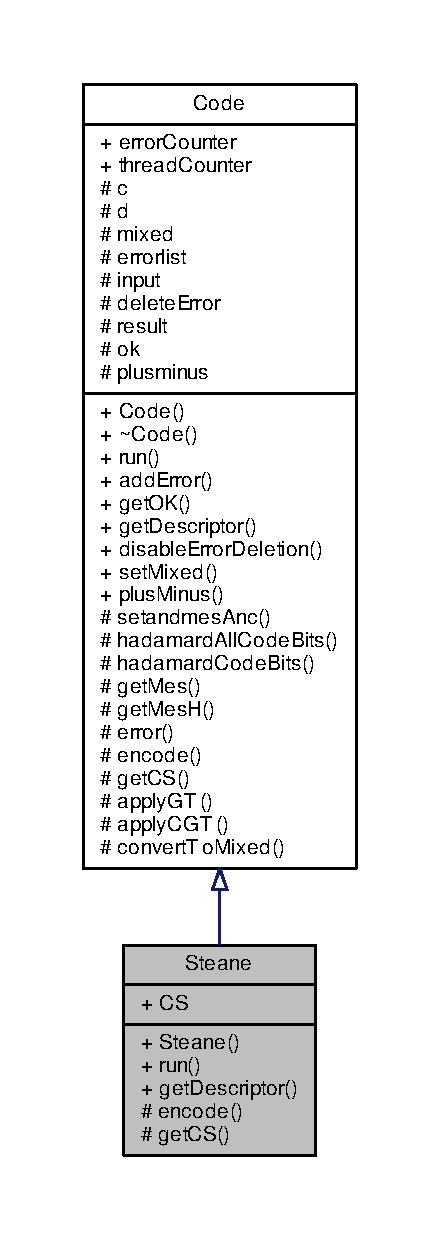
\includegraphics[height=550pt]{class_steane__inherit__graph}
\end{center}
\end{figure}
\subsection*{Public Member Functions}
\begin{DoxyCompactItemize}
\item 
\hyperlink{class_steane_a7cda04d9619fc019d03e16f137851762}{Steane} (bool b)
\item 
bool \hyperlink{class_steane_a0d891a1213b62e1b225fab265fab3fc9}{run} () override
\item 
std\+::string \hyperlink{class_steane_a1fb53da78a66d64cd6aad02735fab4c3}{get\+Descriptor} () override
\end{DoxyCompactItemize}
\subsection*{Static Public Attributes}
\begin{DoxyCompactItemize}
\item 
static const int \hyperlink{class_steane_a3b81ad6daffc03833cea9c333f2cd927}{CS} = 7
\end{DoxyCompactItemize}
\subsection*{Protected Member Functions}
\begin{DoxyCompactItemize}
\item 
void \hyperlink{class_steane_a3c64f20d7329b609984f115cd35651ab}{encode} (bool b) override
\item 
unsigned \hyperlink{class_steane_a7b84b86f9d9737890a146e11479683e6}{get\+CS} () override
\end{DoxyCompactItemize}
\subsection*{Additional Inherited Members}


\subsection{Detailed Description}
!\+Steane code class 

\subsection{Constructor \& Destructor Documentation}
\index{Steane@{Steane}!Steane@{Steane}}
\index{Steane@{Steane}!Steane@{Steane}}
\subsubsection[{\texorpdfstring{Steane(bool b)}{Steane(bool b)}}]{\setlength{\rightskip}{0pt plus 5cm}Steane\+::\+Steane (
\begin{DoxyParamCaption}
\item[{bool}]{b}
\end{DoxyParamCaption}
)\hspace{0.3cm}{\ttfamily [inline]}}\hypertarget{class_steane_a7cda04d9619fc019d03e16f137851762}{}\label{class_steane_a7cda04d9619fc019d03e16f137851762}


\subsection{Member Function Documentation}
\index{Steane@{Steane}!encode@{encode}}
\index{encode@{encode}!Steane@{Steane}}
\subsubsection[{\texorpdfstring{encode(bool b) override}{encode(bool b) override}}]{\setlength{\rightskip}{0pt plus 5cm}void Steane\+::encode (
\begin{DoxyParamCaption}
\item[{bool}]{b}
\end{DoxyParamCaption}
)\hspace{0.3cm}{\ttfamily [override]}, {\ttfamily [protected]}, {\ttfamily [virtual]}}\hypertarget{class_steane_a3c64f20d7329b609984f115cd35651ab}{}\label{class_steane_a3c64f20d7329b609984f115cd35651ab}
Encode input bit 
\begin{DoxyParams}{Parameters}
{\em b} & Classical input converted to $\vert$0$>$ or $\vert$1$>$ \\
\hline
\end{DoxyParams}


Implements \hyperlink{class_code_a5f90b0f96002c9b999d8ed7bab319906}{Code}.

\index{Steane@{Steane}!get\+CS@{get\+CS}}
\index{get\+CS@{get\+CS}!Steane@{Steane}}
\subsubsection[{\texorpdfstring{get\+C\+S() override}{getCS() override}}]{\setlength{\rightskip}{0pt plus 5cm}unsigned Steane\+::get\+CS (
\begin{DoxyParamCaption}
{}
\end{DoxyParamCaption}
)\hspace{0.3cm}{\ttfamily [inline]}, {\ttfamily [override]}, {\ttfamily [protected]}, {\ttfamily [virtual]}}\hypertarget{class_steane_a7b84b86f9d9737890a146e11479683e6}{}\label{class_steane_a7b84b86f9d9737890a146e11479683e6}
Return code size of a child \begin{DoxyReturn}{Returns}
code size 
\end{DoxyReturn}


Implements \hyperlink{class_code_a34f52b25d78aeaec3c1fd381f025ad00}{Code}.

\index{Steane@{Steane}!get\+Descriptor@{get\+Descriptor}}
\index{get\+Descriptor@{get\+Descriptor}!Steane@{Steane}}
\subsubsection[{\texorpdfstring{get\+Descriptor() override}{getDescriptor() override}}]{\setlength{\rightskip}{0pt plus 5cm}std\+::string Steane\+::get\+Descriptor (
\begin{DoxyParamCaption}
{}
\end{DoxyParamCaption}
)\hspace{0.3cm}{\ttfamily [override]}, {\ttfamily [virtual]}}\hypertarget{class_steane_a1fb53da78a66d64cd6aad02735fab4c3}{}\label{class_steane_a1fb53da78a66d64cd6aad02735fab4c3}
Returns a descriptor string~\newline
 Format\+:~\newline
 {\itshape S\+T\+E\+A\+NE xxx zzz i-\/$>$o O\+K/\+E\+R\+R\+OR}~\newline
 Where xxx is xflip, zzz is zflip 

Implements \hyperlink{class_code_a60db2f615a7cff76e3ece1c486b2fd16}{Code}.

\index{Steane@{Steane}!run@{run}}
\index{run@{run}!Steane@{Steane}}
\subsubsection[{\texorpdfstring{run() override}{run() override}}]{\setlength{\rightskip}{0pt plus 5cm}bool Steane\+::run (
\begin{DoxyParamCaption}
{}
\end{DoxyParamCaption}
)\hspace{0.3cm}{\ttfamily [override]}, {\ttfamily [virtual]}}\hypertarget{class_steane_a0d891a1213b62e1b225fab265fab3fc9}{}\label{class_steane_a0d891a1213b62e1b225fab265fab3fc9}
Function to simulate the transmission and get the result. To be defined in child classes. \begin{DoxyReturn}{Returns}
Measured bit at Bob 
\end{DoxyReturn}


Implements \hyperlink{class_code_a5621bbd050948ba1e41f69f451a05990}{Code}.



\subsection{Member Data Documentation}
\index{Steane@{Steane}!CS@{CS}}
\index{CS@{CS}!Steane@{Steane}}
\subsubsection[{\texorpdfstring{CS}{CS}}]{\setlength{\rightskip}{0pt plus 5cm}const int Steane\+::\+CS = 7\hspace{0.3cm}{\ttfamily [static]}}\hypertarget{class_steane_a3b81ad6daffc03833cea9c333f2cd927}{}\label{class_steane_a3b81ad6daffc03833cea9c333f2cd927}
\hyperlink{class_code}{Code} size for steane is 7 

The documentation for this class was generated from the following files\+:\begin{DoxyCompactItemize}
\item 
/home/attila/src/qecc-\/netbeans/qecc/\hyperlink{_steane_8h}{Steane.\+h}\item 
/home/attila/src/qecc-\/netbeans/qecc/\hyperlink{_steane_8cpp}{Steane.\+cpp}\end{DoxyCompactItemize}

\hypertarget{class_test}{}\section{Test Class Reference}
\label{class_test}\index{Test@{Test}}


{\ttfamily \#include $<$Test.\+h$>$}



Inheritance diagram for Test\+:\nopagebreak
\begin{figure}[H]
\begin{center}
\leavevmode
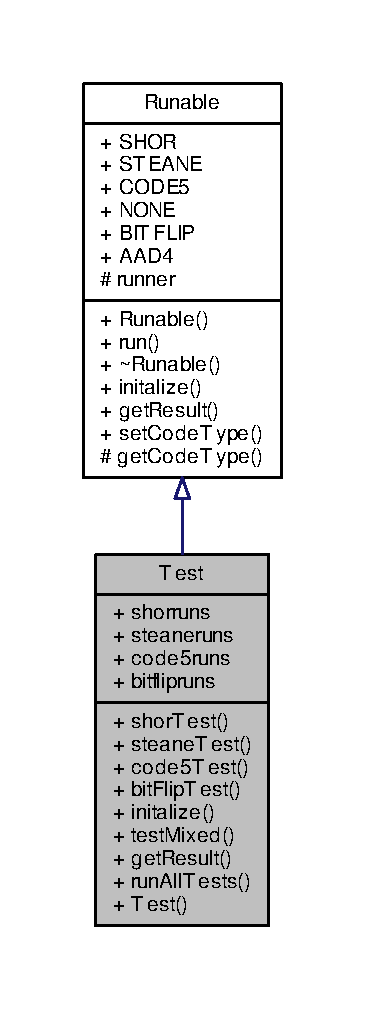
\includegraphics[width=175pt]{class_test__inherit__graph}
\end{center}
\end{figure}
\subsection*{Public Member Functions}
\begin{DoxyCompactItemize}
\item 
void \hyperlink{class_test_aac2e651b089febf2cd5ab1b5d2874c5a}{shor\+Test} (bool input)
\item 
void \hyperlink{class_test_a9bac2c6bc99fbb7f54b79712006956c0}{steane\+Test} (bool input)
\item 
void \hyperlink{class_test_a784d32490d6aa0bf8909d6a1cad5ee33}{code5\+Test} (bool input)
\item 
void \hyperlink{class_test_a89dd7059b847c8429636007515cd42ac}{bit\+Flip\+Test} (bool input)
\item 
void \hyperlink{class_test_a6baf4b2ddf84f198e156bf78c97b865b}{initalize} () override
\item 
void \hyperlink{class_test_afd06ee055f93c52fca29ffd2266b5564}{test\+Mixed} ()
\item 
std\+::string \hyperlink{class_test_ae53178c2e482ed3a869c742387521a60}{get\+Result} () override
\item 
void \hyperlink{class_test_a2616b0b705d644091904f3de58eb46bb}{run\+All\+Tests} ()
\item 
\hyperlink{class_test_ab61976fd1ea38385bd4260d433f930c0}{Test} (int type, int maxnumthreads)
\end{DoxyCompactItemize}
\subsection*{Static Public Attributes}
\begin{DoxyCompactItemize}
\item 
static const int \hyperlink{class_test_af926faddaa7288d10542e78bc1be29f6}{shorruns} = 4 $\ast$ \hyperlink{class_shor_a5c2bb5ad73004577f8781a001eda8b8f}{Shor\+::\+CS} + 6
\item 
static const int \hyperlink{class_test_a1f5e5c6be1ad2c4459ad702c254c72a1}{steaneruns} = 5 $\ast$ \hyperlink{class_steane_a3b81ad6daffc03833cea9c333f2cd927}{Steane\+::\+CS}
\item 
static const int \hyperlink{class_test_af99add0cf16991621c26ea17bd38d41d}{code5runs} = 4 $\ast$ \hyperlink{class_code5_ac252f1c41568341657456564d0417630}{Code5\+::\+CS}
\item 
static const int \hyperlink{class_test_af4a50e78867431da5e5b8cf5110645aa}{bitflipruns} = \hyperlink{class_bit_flip_a8f5442dd93f87ea35fcb0b0bb423bbf0}{Bit\+Flip\+::\+CS}
\end{DoxyCompactItemize}
\subsection*{Additional Inherited Members}


\subsection{Detailed Description}
Runs tests for codes 

\subsection{Constructor \& Destructor Documentation}
\index{Test@{Test}!Test@{Test}}
\index{Test@{Test}!Test@{Test}}
\subsubsection[{\texorpdfstring{Test(int type, int maxnumthreads)}{Test(int type, int maxnumthreads)}}]{\setlength{\rightskip}{0pt plus 5cm}Test\+::\+Test (
\begin{DoxyParamCaption}
\item[{int}]{type, }
\item[{int}]{maxnumthreads}
\end{DoxyParamCaption}
)\hspace{0.3cm}{\ttfamily [inline]}}\hypertarget{class_test_ab61976fd1ea38385bd4260d433f930c0}{}\label{class_test_ab61976fd1ea38385bd4260d433f930c0}

\begin{DoxyParams}{Parameters}
{\em type} & \hyperlink{class_code}{Code} type \\
\hline
{\em maxnumthreads} & Maximum number of threads \\
\hline
\end{DoxyParams}


\subsection{Member Function Documentation}
\index{Test@{Test}!bit\+Flip\+Test@{bit\+Flip\+Test}}
\index{bit\+Flip\+Test@{bit\+Flip\+Test}!Test@{Test}}
\subsubsection[{\texorpdfstring{bit\+Flip\+Test(bool input)}{bitFlipTest(bool input)}}]{\setlength{\rightskip}{0pt plus 5cm}void Test\+::bit\+Flip\+Test (
\begin{DoxyParamCaption}
\item[{bool}]{input}
\end{DoxyParamCaption}
)}\hypertarget{class_test_a89dd7059b847c8429636007515cd42ac}{}\label{class_test_a89dd7059b847c8429636007515cd42ac}
Initialize for bit flip 
\begin{DoxyParams}{Parameters}
{\em input} & input bit \\
\hline
\end{DoxyParams}
\index{Test@{Test}!code5\+Test@{code5\+Test}}
\index{code5\+Test@{code5\+Test}!Test@{Test}}
\subsubsection[{\texorpdfstring{code5\+Test(bool input)}{code5Test(bool input)}}]{\setlength{\rightskip}{0pt plus 5cm}void Test\+::code5\+Test (
\begin{DoxyParamCaption}
\item[{bool}]{input}
\end{DoxyParamCaption}
)}\hypertarget{class_test_a784d32490d6aa0bf8909d6a1cad5ee33}{}\label{class_test_a784d32490d6aa0bf8909d6a1cad5ee33}
Initialize for 5\+Qubit 
\begin{DoxyParams}{Parameters}
{\em input} & input bit \\
\hline
\end{DoxyParams}
\index{Test@{Test}!get\+Result@{get\+Result}}
\index{get\+Result@{get\+Result}!Test@{Test}}
\subsubsection[{\texorpdfstring{get\+Result() override}{getResult() override}}]{\setlength{\rightskip}{0pt plus 5cm}std\+::string Test\+::get\+Result (
\begin{DoxyParamCaption}
{}
\end{DoxyParamCaption}
)\hspace{0.3cm}{\ttfamily [inline]}, {\ttfamily [override]}, {\ttfamily [virtual]}}\hypertarget{class_test_ae53178c2e482ed3a869c742387521a60}{}\label{class_test_ae53178c2e482ed3a869c742387521a60}
Descriptor string~\newline
 If all are okay {\bfseries T\+E\+ST S\+U\+C\+C\+E\+S\+F\+U\+LL}~\newline
 If some failed {\bfseries S\+O\+ME T\+E\+S\+TS F\+A\+I\+L\+ED} \begin{DoxyReturn}{Returns}

\end{DoxyReturn}


Implements \hyperlink{class_runable_a761a0c657253223f3dd7cf2c0762c34e}{Runable}.

\index{Test@{Test}!initalize@{initalize}}
\index{initalize@{initalize}!Test@{Test}}
\subsubsection[{\texorpdfstring{initalize() override}{initalize() override}}]{\setlength{\rightskip}{0pt plus 5cm}void Test\+::initalize (
\begin{DoxyParamCaption}
{}
\end{DoxyParamCaption}
)\hspace{0.3cm}{\ttfamily [override]}, {\ttfamily [virtual]}}\hypertarget{class_test_a6baf4b2ddf84f198e156bf78c97b865b}{}\label{class_test_a6baf4b2ddf84f198e156bf78c97b865b}
Initalizes code list. To be defined by child! 

Implements \hyperlink{class_runable_ae45ce89bb273ba5863e8ca0951caef85}{Runable}.

\index{Test@{Test}!run\+All\+Tests@{run\+All\+Tests}}
\index{run\+All\+Tests@{run\+All\+Tests}!Test@{Test}}
\subsubsection[{\texorpdfstring{run\+All\+Tests()}{runAllTests()}}]{\setlength{\rightskip}{0pt plus 5cm}void Test\+::run\+All\+Tests (
\begin{DoxyParamCaption}
{}
\end{DoxyParamCaption}
)}\hypertarget{class_test_a2616b0b705d644091904f3de58eb46bb}{}\label{class_test_a2616b0b705d644091904f3de58eb46bb}
Runs all inbuilt tests \index{Test@{Test}!shor\+Test@{shor\+Test}}
\index{shor\+Test@{shor\+Test}!Test@{Test}}
\subsubsection[{\texorpdfstring{shor\+Test(bool input)}{shorTest(bool input)}}]{\setlength{\rightskip}{0pt plus 5cm}void Test\+::shor\+Test (
\begin{DoxyParamCaption}
\item[{bool}]{input}
\end{DoxyParamCaption}
)}\hypertarget{class_test_aac2e651b089febf2cd5ab1b5d2874c5a}{}\label{class_test_aac2e651b089febf2cd5ab1b5d2874c5a}
Initialize for shor 
\begin{DoxyParams}{Parameters}
{\em input} & input bit \\
\hline
\end{DoxyParams}
\index{Test@{Test}!steane\+Test@{steane\+Test}}
\index{steane\+Test@{steane\+Test}!Test@{Test}}
\subsubsection[{\texorpdfstring{steane\+Test(bool input)}{steaneTest(bool input)}}]{\setlength{\rightskip}{0pt plus 5cm}void Test\+::steane\+Test (
\begin{DoxyParamCaption}
\item[{bool}]{input}
\end{DoxyParamCaption}
)}\hypertarget{class_test_a9bac2c6bc99fbb7f54b79712006956c0}{}\label{class_test_a9bac2c6bc99fbb7f54b79712006956c0}
Initialize for steane 
\begin{DoxyParams}{Parameters}
{\em input} & input bit \\
\hline
\end{DoxyParams}
\index{Test@{Test}!test\+Mixed@{test\+Mixed}}
\index{test\+Mixed@{test\+Mixed}!Test@{Test}}
\subsubsection[{\texorpdfstring{test\+Mixed()}{testMixed()}}]{\setlength{\rightskip}{0pt plus 5cm}void Test\+::test\+Mixed (
\begin{DoxyParamCaption}
{}
\end{DoxyParamCaption}
)\hspace{0.3cm}{\ttfamily [inline]}}\hypertarget{class_test_afd06ee055f93c52fca29ffd2266b5564}{}\label{class_test_afd06ee055f93c52fca29ffd2266b5564}
Run tests using density matrix notation 

\subsection{Member Data Documentation}
\index{Test@{Test}!bitflipruns@{bitflipruns}}
\index{bitflipruns@{bitflipruns}!Test@{Test}}
\subsubsection[{\texorpdfstring{bitflipruns}{bitflipruns}}]{\setlength{\rightskip}{0pt plus 5cm}const int Test\+::bitflipruns = {\bf Bit\+Flip\+::\+CS}\hspace{0.3cm}{\ttfamily [static]}}\hypertarget{class_test_af4a50e78867431da5e5b8cf5110645aa}{}\label{class_test_af4a50e78867431da5e5b8cf5110645aa}
Number of runs for bit flip code \index{Test@{Test}!code5runs@{code5runs}}
\index{code5runs@{code5runs}!Test@{Test}}
\subsubsection[{\texorpdfstring{code5runs}{code5runs}}]{\setlength{\rightskip}{0pt plus 5cm}const int Test\+::code5runs = 4 $\ast$ {\bf Code5\+::\+CS}\hspace{0.3cm}{\ttfamily [static]}}\hypertarget{class_test_af99add0cf16991621c26ea17bd38d41d}{}\label{class_test_af99add0cf16991621c26ea17bd38d41d}
Number of runs for 5\+Qubit code \index{Test@{Test}!shorruns@{shorruns}}
\index{shorruns@{shorruns}!Test@{Test}}
\subsubsection[{\texorpdfstring{shorruns}{shorruns}}]{\setlength{\rightskip}{0pt plus 5cm}const int Test\+::shorruns = 4 $\ast$ {\bf Shor\+::\+CS} + 6\hspace{0.3cm}{\ttfamily [static]}}\hypertarget{class_test_af926faddaa7288d10542e78bc1be29f6}{}\label{class_test_af926faddaa7288d10542e78bc1be29f6}
Number of runs for \hyperlink{class_shor}{Shor} code \index{Test@{Test}!steaneruns@{steaneruns}}
\index{steaneruns@{steaneruns}!Test@{Test}}
\subsubsection[{\texorpdfstring{steaneruns}{steaneruns}}]{\setlength{\rightskip}{0pt plus 5cm}const int Test\+::steaneruns = 5 $\ast$ {\bf Steane\+::\+CS}\hspace{0.3cm}{\ttfamily [static]}}\hypertarget{class_test_a1f5e5c6be1ad2c4459ad702c254c72a1}{}\label{class_test_a1f5e5c6be1ad2c4459ad702c254c72a1}
Number of runs for steane code 

The documentation for this class was generated from the following files\+:\begin{DoxyCompactItemize}
\item 
/home/attila/src/qecc-\/netbeans/qecc/\hyperlink{_test_8h}{Test.\+h}\item 
/home/attila/src/qecc-\/netbeans/qecc/\hyperlink{_test_8cpp}{Test.\+cpp}\end{DoxyCompactItemize}

\chapter{File Documentation}
\hypertarget{_8dep_8inc}{}\section{/home/attila/src/qecc-\/netbeans/qecc/.dep.\+inc File Reference}
\label{_8dep_8inc}\index{/home/attila/src/qecc-\/netbeans/qecc/.\+dep.\+inc@{/home/attila/src/qecc-\/netbeans/qecc/.\+dep.\+inc}}

\hypertarget{_aad4_8cpp}{}\section{/home/attila/src/qecc-\/netbeans/qecc/\+Aad4.cpp File Reference}
\label{_aad4_8cpp}\index{/home/attila/src/qecc-\/netbeans/qecc/\+Aad4.\+cpp@{/home/attila/src/qecc-\/netbeans/qecc/\+Aad4.\+cpp}}
{\ttfamily \#include \char`\"{}Aad4.\+h\char`\"{}}\\*
{\ttfamily \#include $<$complex$>$}\\*
{\ttfamily \#include $<$math.\+h$>$}\\*

\hypertarget{_aad4_8h}{}\section{/home/attila/src/qecc-\/netbeans/qecc/\+Aad4.h File Reference}
\label{_aad4_8h}\index{/home/attila/src/qecc-\/netbeans/qecc/\+Aad4.\+h@{/home/attila/src/qecc-\/netbeans/qecc/\+Aad4.\+h}}
{\ttfamily \#include \char`\"{}qpp.\+h\char`\"{}}\\*
{\ttfamily \#include \char`\"{}Code.\+h\char`\"{}}\\*
\subsection*{Classes}
\begin{DoxyCompactItemize}
\item 
class \hyperlink{class_aad4}{Aad4}
\end{DoxyCompactItemize}

\hypertarget{_bit_flip_8cpp}{}\section{/home/attila/src/qecc-\/netbeans/qecc/\+Bit\+Flip.cpp File Reference}
\label{_bit_flip_8cpp}\index{/home/attila/src/qecc-\/netbeans/qecc/\+Bit\+Flip.\+cpp@{/home/attila/src/qecc-\/netbeans/qecc/\+Bit\+Flip.\+cpp}}
{\ttfamily \#include \char`\"{}Bit\+Flip.\+h\char`\"{}}\\*

\hypertarget{_bit_flip_8h}{}\section{/home/attila/src/qecc-\/netbeans/qecc/\+Bit\+Flip.h File Reference}
\label{_bit_flip_8h}\index{/home/attila/src/qecc-\/netbeans/qecc/\+Bit\+Flip.\+h@{/home/attila/src/qecc-\/netbeans/qecc/\+Bit\+Flip.\+h}}
{\ttfamily \#include \char`\"{}qpp.\+h\char`\"{}}\\*
{\ttfamily \#include \char`\"{}Code.\+h\char`\"{}}\\*
{\ttfamily \#include $<$iostream$>$}\\*
\subsection*{Classes}
\begin{DoxyCompactItemize}
\item 
class \hyperlink{class_bit_flip}{Bit\+Flip}
\end{DoxyCompactItemize}

\hypertarget{_channel_8cpp}{}\section{/home/attila/src/qecc-\/netbeans/qecc/\+Channel.cpp File Reference}
\label{_channel_8cpp}\index{/home/attila/src/qecc-\/netbeans/qecc/\+Channel.\+cpp@{/home/attila/src/qecc-\/netbeans/qecc/\+Channel.\+cpp}}
{\ttfamily \#include \char`\"{}Channel.\+h\char`\"{}}\\*

\hypertarget{_channel_8h}{}\section{/home/attila/src/qecc-\/netbeans/qecc/\+Channel.h File Reference}
\label{_channel_8h}\index{/home/attila/src/qecc-\/netbeans/qecc/\+Channel.\+h@{/home/attila/src/qecc-\/netbeans/qecc/\+Channel.\+h}}
{\ttfamily \#include \char`\"{}Error.\+h\char`\"{}}\\*
{\ttfamily \#include \char`\"{}Node.\+h\char`\"{}}\\*
{\ttfamily \#include $<$queue$>$}\\*
\subsection*{Classes}
\begin{DoxyCompactItemize}
\item 
class \hyperlink{class_channel}{Channel}
\end{DoxyCompactItemize}

\hypertarget{_code_8cpp}{}\section{/home/attila/src/qecc-\/netbeans/qecc/\+Code.cpp File Reference}
\label{_code_8cpp}\index{/home/attila/src/qecc-\/netbeans/qecc/\+Code.\+cpp@{/home/attila/src/qecc-\/netbeans/qecc/\+Code.\+cpp}}
{\ttfamily \#include \char`\"{}Code.\+h\char`\"{}}\\*

\hypertarget{_code_8h}{}\section{/home/attila/src/qecc-\/netbeans/qecc/\+Code.h File Reference}
\label{_code_8h}\index{/home/attila/src/qecc-\/netbeans/qecc/\+Code.\+h@{/home/attila/src/qecc-\/netbeans/qecc/\+Code.\+h}}
{\ttfamily \#include \char`\"{}qpp.\+h\char`\"{}}\\*
{\ttfamily \#include \char`\"{}Error.\+h\char`\"{}}\\*
{\ttfamily \#include $<$iostream$>$}\\*
{\ttfamily \#include $<$queue$>$}\\*
{\ttfamily \#include $<$atomic$>$}\\*
\subsection*{Classes}
\begin{DoxyCompactItemize}
\item 
class \hyperlink{class_code}{Code}
\end{DoxyCompactItemize}

\hypertarget{_code5_8cpp}{}\section{/home/attila/src/qecc-\/netbeans/qecc/\+Code5.cpp File Reference}
\label{_code5_8cpp}\index{/home/attila/src/qecc-\/netbeans/qecc/\+Code5.\+cpp@{/home/attila/src/qecc-\/netbeans/qecc/\+Code5.\+cpp}}
{\ttfamily \#include \char`\"{}Code5.\+h\char`\"{}}\\*

\hypertarget{_code5_8h}{}\section{/home/attila/src/qecc-\/netbeans/qecc/\+Code5.h File Reference}
\label{_code5_8h}\index{/home/attila/src/qecc-\/netbeans/qecc/\+Code5.\+h@{/home/attila/src/qecc-\/netbeans/qecc/\+Code5.\+h}}
{\ttfamily \#include \char`\"{}qpp.\+h\char`\"{}}\\*
{\ttfamily \#include \char`\"{}Code.\+h\char`\"{}}\\*
{\ttfamily \#include $<$iostream$>$}\\*
\subsection*{Classes}
\begin{DoxyCompactItemize}
\item 
class \hyperlink{class_code5}{Code5}
\end{DoxyCompactItemize}

\hypertarget{_error_8cpp}{}\section{/home/attila/src/qecc-\/netbeans/qecc/\+Error.cpp File Reference}
\label{_error_8cpp}\index{/home/attila/src/qecc-\/netbeans/qecc/\+Error.\+cpp@{/home/attila/src/qecc-\/netbeans/qecc/\+Error.\+cpp}}
{\ttfamily \#include \char`\"{}Error.\+h\char`\"{}}\\*
{\ttfamily \#include \char`\"{}Code.\+h\char`\"{}}\\*

\hypertarget{_error_8h}{}\section{/home/attila/src/qecc-\/netbeans/qecc/\+Error.h File Reference}
\label{_error_8h}\index{/home/attila/src/qecc-\/netbeans/qecc/\+Error.\+h@{/home/attila/src/qecc-\/netbeans/qecc/\+Error.\+h}}
{\ttfamily \#include \char`\"{}qpp.\+h\char`\"{}}\\*
\subsection*{Classes}
\begin{DoxyCompactItemize}
\item 
class \hyperlink{class_error}{Error}
\end{DoxyCompactItemize}

\hypertarget{_network_8cpp}{}\section{/home/attila/src/qecc-\/netbeans/qecc/\+Network.cpp File Reference}
\label{_network_8cpp}\index{/home/attila/src/qecc-\/netbeans/qecc/\+Network.\+cpp@{/home/attila/src/qecc-\/netbeans/qecc/\+Network.\+cpp}}
{\ttfamily \#include \char`\"{}Network.\+h\char`\"{}}\\*
{\ttfamily \#include $<$fstream$>$}\\*
{\ttfamily \#include $<$list$>$}\\*
{\ttfamily \#include \char`\"{}Steane.\+h\char`\"{}}\\*
{\ttfamily \#include \char`\"{}Shor.\+h\char`\"{}}\\*
{\ttfamily \#include \char`\"{}Code5.\+h\char`\"{}}\\*
{\ttfamily \#include \char`\"{}Bit\+Flip.\+h\char`\"{}}\\*
{\ttfamily \#include \char`\"{}Code.\+h\char`\"{}}\\*
{\ttfamily \#include \char`\"{}None.\+h\char`\"{}}\\*
{\ttfamily \#include \char`\"{}Aad4.\+h\char`\"{}}\\*

\hypertarget{_network_8h}{}\section{/home/attila/src/qecc-\/netbeans/qecc/\+Network.h File Reference}
\label{_network_8h}\index{/home/attila/src/qecc-\/netbeans/qecc/\+Network.\+h@{/home/attila/src/qecc-\/netbeans/qecc/\+Network.\+h}}
{\ttfamily \#include \char`\"{}Node.\+h\char`\"{}}\\*
{\ttfamily \#include \char`\"{}Channel.\+h\char`\"{}}\\*
{\ttfamily \#include \char`\"{}Runable.\+h\char`\"{}}\\*
{\ttfamily \#include $<$list$>$}\\*
\subsection*{Classes}
\begin{DoxyCompactItemize}
\item 
class \hyperlink{class_network}{Network}
\end{DoxyCompactItemize}

\hypertarget{_node_8cpp}{}\section{/home/attila/src/qecc-\/netbeans/qecc/\+Node.cpp File Reference}
\label{_node_8cpp}\index{/home/attila/src/qecc-\/netbeans/qecc/\+Node.\+cpp@{/home/attila/src/qecc-\/netbeans/qecc/\+Node.\+cpp}}
{\ttfamily \#include \char`\"{}Node.\+h\char`\"{}}\\*

\hypertarget{_node_8h}{}\section{/home/attila/src/qecc-\/netbeans/qecc/\+Node.h File Reference}
\label{_node_8h}\index{/home/attila/src/qecc-\/netbeans/qecc/\+Node.\+h@{/home/attila/src/qecc-\/netbeans/qecc/\+Node.\+h}}
{\ttfamily \#include $<$atomic$>$}\\*
{\ttfamily \#include $<$string$>$}\\*
\subsection*{Classes}
\begin{DoxyCompactItemize}
\item 
class \hyperlink{class_node}{Node}
\end{DoxyCompactItemize}

\hypertarget{_none_8cpp}{}\section{/home/attila/src/qecc-\/netbeans/qecc/\+None.cpp File Reference}
\label{_none_8cpp}\index{/home/attila/src/qecc-\/netbeans/qecc/\+None.\+cpp@{/home/attila/src/qecc-\/netbeans/qecc/\+None.\+cpp}}
{\ttfamily \#include \char`\"{}None.\+h\char`\"{}}\\*

\hypertarget{_none_8h}{}\section{/home/attila/src/qecc-\/netbeans/qecc/\+None.h File Reference}
\label{_none_8h}\index{/home/attila/src/qecc-\/netbeans/qecc/\+None.\+h@{/home/attila/src/qecc-\/netbeans/qecc/\+None.\+h}}
{\ttfamily \#include \char`\"{}qpp.\+h\char`\"{}}\\*
{\ttfamily \#include \char`\"{}Code.\+h\char`\"{}}\\*
{\ttfamily \#include $<$iostream$>$}\\*
\subsection*{Classes}
\begin{DoxyCompactItemize}
\item 
class \hyperlink{class_none}{None}
\end{DoxyCompactItemize}

\hypertarget{qecc_8cpp}{}\section{/home/attila/src/qecc-\/netbeans/qecc/qecc.cpp File Reference}
\label{qecc_8cpp}\index{/home/attila/src/qecc-\/netbeans/qecc/qecc.\+cpp@{/home/attila/src/qecc-\/netbeans/qecc/qecc.\+cpp}}
{\ttfamily \#include $<$cstdlib$>$}\\*
{\ttfamily \#include \char`\"{}Shor.\+h\char`\"{}}\\*
{\ttfamily \#include \char`\"{}Steane.\+h\char`\"{}}\\*
{\ttfamily \#include \char`\"{}Code.\+h\char`\"{}}\\*
{\ttfamily \#include \char`\"{}Code5.\+h\char`\"{}}\\*
{\ttfamily \#include \char`\"{}None.\+h\char`\"{}}\\*
{\ttfamily \#include \char`\"{}Runner.\+h\char`\"{}}\\*
{\ttfamily \#include \char`\"{}Test.\+h\char`\"{}}\\*
{\ttfamily \#include $<$iostream$>$}\\*
{\ttfamily \#include $<$unistd.\+h$>$}\\*
{\ttfamily \#include \char`\"{}Single.\+h\char`\"{}}\\*
{\ttfamily \#include \char`\"{}Network.\+h\char`\"{}}\\*
\subsection*{Functions}
\begin{DoxyCompactItemize}
\item 
void \hyperlink{qecc_8cpp_a0d20b69b0ad703df78459e1033d5c1d4}{print\+Help} ()
\item 
int \hyperlink{qecc_8cpp_a3c04138a5bfe5d72780bb7e82a18e627}{main} (int argc, char $\ast$$\ast$argv)
\end{DoxyCompactItemize}
\subsection*{Variables}
\begin{DoxyCompactItemize}
\item 
volatile int \hyperlink{qecc_8cpp_a8185543200d06aa88de09672d53fc5f8}{numthreads} = 0
\item 
volatile int \hyperlink{qecc_8cpp_a7ffaff0c74104cca0e85dd9249bd964f}{err\+Run} = 0
\end{DoxyCompactItemize}


\subsection{Function Documentation}
\index{qecc.\+cpp@{qecc.\+cpp}!main@{main}}
\index{main@{main}!qecc.\+cpp@{qecc.\+cpp}}
\subsubsection[{\texorpdfstring{main(int argc, char $\ast$$\ast$argv)}{main(int argc, char **argv)}}]{\setlength{\rightskip}{0pt plus 5cm}int main (
\begin{DoxyParamCaption}
\item[{int}]{argc, }
\item[{char $\ast$$\ast$}]{argv}
\end{DoxyParamCaption}
)}\hypertarget{qecc_8cpp_a3c04138a5bfe5d72780bb7e82a18e627}{}\label{qecc_8cpp_a3c04138a5bfe5d72780bb7e82a18e627}
Main function of qecc 
\begin{DoxyParams}{Parameters}
{\em argc} & \\
\hline
{\em argv} & \\
\hline
\end{DoxyParams}
\begin{DoxyReturn}{Returns}

\end{DoxyReturn}
\index{qecc.\+cpp@{qecc.\+cpp}!print\+Help@{print\+Help}}
\index{print\+Help@{print\+Help}!qecc.\+cpp@{qecc.\+cpp}}
\subsubsection[{\texorpdfstring{print\+Help()}{printHelp()}}]{\setlength{\rightskip}{0pt plus 5cm}void print\+Help (
\begin{DoxyParamCaption}
{}
\end{DoxyParamCaption}
)}\hypertarget{qecc_8cpp_a0d20b69b0ad703df78459e1033d5c1d4}{}\label{qecc_8cpp_a0d20b69b0ad703df78459e1033d5c1d4}
Print help for qecc 

\subsection{Variable Documentation}
\index{qecc.\+cpp@{qecc.\+cpp}!err\+Run@{err\+Run}}
\index{err\+Run@{err\+Run}!qecc.\+cpp@{qecc.\+cpp}}
\subsubsection[{\texorpdfstring{err\+Run}{errRun}}]{\setlength{\rightskip}{0pt plus 5cm}volatile int err\+Run = 0}\hypertarget{qecc_8cpp_a7ffaff0c74104cca0e85dd9249bd964f}{}\label{qecc_8cpp_a7ffaff0c74104cca0e85dd9249bd964f}
\index{qecc.\+cpp@{qecc.\+cpp}!numthreads@{numthreads}}
\index{numthreads@{numthreads}!qecc.\+cpp@{qecc.\+cpp}}
\subsubsection[{\texorpdfstring{numthreads}{numthreads}}]{\setlength{\rightskip}{0pt plus 5cm}volatile int numthreads = 0}\hypertarget{qecc_8cpp_a8185543200d06aa88de09672d53fc5f8}{}\label{qecc_8cpp_a8185543200d06aa88de09672d53fc5f8}

\hypertarget{_r_e_a_d_m_e_8md}{}\section{/home/attila/src/qecc-\/netbeans/qecc/\+R\+E\+A\+D\+ME.md File Reference}
\label{_r_e_a_d_m_e_8md}\index{/home/attila/src/qecc-\/netbeans/qecc/\+R\+E\+A\+D\+M\+E.\+md@{/home/attila/src/qecc-\/netbeans/qecc/\+R\+E\+A\+D\+M\+E.\+md}}

\hypertarget{_runable_8cpp}{}\section{/home/attila/src/qecc-\/netbeans/qecc/\+Runable.cpp File Reference}
\label{_runable_8cpp}\index{/home/attila/src/qecc-\/netbeans/qecc/\+Runable.\+cpp@{/home/attila/src/qecc-\/netbeans/qecc/\+Runable.\+cpp}}
{\ttfamily \#include \char`\"{}Runable.\+h\char`\"{}}\\*

\hypertarget{_runable_8h}{}\section{/home/attila/src/qecc-\/netbeans/qecc/\+Runable.h File Reference}
\label{_runable_8h}\index{/home/attila/src/qecc-\/netbeans/qecc/\+Runable.\+h@{/home/attila/src/qecc-\/netbeans/qecc/\+Runable.\+h}}
{\ttfamily \#include \char`\"{}Runner.\+h\char`\"{}}\\*
\subsection*{Classes}
\begin{DoxyCompactItemize}
\item 
class \hyperlink{class_runable}{Runable}
\end{DoxyCompactItemize}

\hypertarget{_runner_8cpp}{}\section{/home/attila/src/qecc-\/netbeans/qecc/\+Runner.cpp File Reference}
\label{_runner_8cpp}\index{/home/attila/src/qecc-\/netbeans/qecc/\+Runner.\+cpp@{/home/attila/src/qecc-\/netbeans/qecc/\+Runner.\+cpp}}
{\ttfamily \#include $<$queue$>$}\\*
{\ttfamily \#include \char`\"{}Runner.\+h\char`\"{}}\\*
{\ttfamily \#include $<$unistd.\+h$>$}\\*
\subsection*{Functions}
\begin{DoxyCompactItemize}
\item 
void $\ast$ \hyperlink{_runner_8cpp_a3ce50b1c8a5b3c60a7506638373c4751}{run\+Code} (void $\ast$c)
\end{DoxyCompactItemize}


\subsection{Function Documentation}
\index{Runner.\+cpp@{Runner.\+cpp}!run\+Code@{run\+Code}}
\index{run\+Code@{run\+Code}!Runner.\+cpp@{Runner.\+cpp}}
\subsubsection[{\texorpdfstring{run\+Code(void $\ast$c)}{runCode(void *c)}}]{\setlength{\rightskip}{0pt plus 5cm}void$\ast$ run\+Code (
\begin{DoxyParamCaption}
\item[{void $\ast$}]{c}
\end{DoxyParamCaption}
)}\hypertarget{_runner_8cpp_a3ce50b1c8a5b3c60a7506638373c4751}{}\label{_runner_8cpp_a3ce50b1c8a5b3c60a7506638373c4751}
Function to be run by \hyperlink{class_runner}{Runner} using pthread 
\begin{DoxyParams}{Parameters}
{\em c} & Pointer to \hyperlink{class_code}{Code} instance to be run \\
\hline
\end{DoxyParams}
\begin{DoxyReturn}{Returns}
Unused 
\end{DoxyReturn}

\hypertarget{_runner_8h}{}\section{/home/attila/src/qecc-\/netbeans/qecc/\+Runner.h File Reference}
\label{_runner_8h}\index{/home/attila/src/qecc-\/netbeans/qecc/\+Runner.\+h@{/home/attila/src/qecc-\/netbeans/qecc/\+Runner.\+h}}
{\ttfamily \#include \char`\"{}Code.\+h\char`\"{}}\\*
\subsection*{Classes}
\begin{DoxyCompactItemize}
\item 
class \hyperlink{class_runner}{Runner}
\end{DoxyCompactItemize}
\subsection*{Functions}
\begin{DoxyCompactItemize}
\item 
void $\ast$ \hyperlink{_runner_8h_a3ce50b1c8a5b3c60a7506638373c4751}{run\+Code} (void $\ast$c)
\end{DoxyCompactItemize}


\subsection{Function Documentation}
\index{Runner.\+h@{Runner.\+h}!run\+Code@{run\+Code}}
\index{run\+Code@{run\+Code}!Runner.\+h@{Runner.\+h}}
\subsubsection[{\texorpdfstring{run\+Code(void $\ast$c)}{runCode(void *c)}}]{\setlength{\rightskip}{0pt plus 5cm}void$\ast$ run\+Code (
\begin{DoxyParamCaption}
\item[{void $\ast$}]{c}
\end{DoxyParamCaption}
)}\hypertarget{_runner_8h_a3ce50b1c8a5b3c60a7506638373c4751}{}\label{_runner_8h_a3ce50b1c8a5b3c60a7506638373c4751}
Function to be run by \hyperlink{class_runner}{Runner} using pthread 
\begin{DoxyParams}{Parameters}
{\em c} & Pointer to \hyperlink{class_code}{Code} instance to be run \\
\hline
\end{DoxyParams}
\begin{DoxyReturn}{Returns}
Unused 
\end{DoxyReturn}

\hypertarget{_shor_8cpp}{}\section{/home/attila/src/qecc-\/netbeans/qecc/\+Shor.cpp File Reference}
\label{_shor_8cpp}\index{/home/attila/src/qecc-\/netbeans/qecc/\+Shor.\+cpp@{/home/attila/src/qecc-\/netbeans/qecc/\+Shor.\+cpp}}
{\ttfamily \#include \char`\"{}Shor.\+h\char`\"{}}\\*

\hypertarget{_shor_8h}{}\section{/home/attila/src/qecc-\/netbeans/qecc/\+Shor.h File Reference}
\label{_shor_8h}\index{/home/attila/src/qecc-\/netbeans/qecc/\+Shor.\+h@{/home/attila/src/qecc-\/netbeans/qecc/\+Shor.\+h}}
{\ttfamily \#include \char`\"{}qpp.\+h\char`\"{}}\\*
{\ttfamily \#include \char`\"{}Code.\+h\char`\"{}}\\*
{\ttfamily \#include $<$iostream$>$}\\*
\subsection*{Classes}
\begin{DoxyCompactItemize}
\item 
class \hyperlink{class_shor}{Shor}
\end{DoxyCompactItemize}

\hypertarget{_single_8cpp}{}\section{/home/attila/src/qecc-\/netbeans/qecc/\+Single.cpp File Reference}
\label{_single_8cpp}\index{/home/attila/src/qecc-\/netbeans/qecc/\+Single.\+cpp@{/home/attila/src/qecc-\/netbeans/qecc/\+Single.\+cpp}}
{\ttfamily \#include \char`\"{}Single.\+h\char`\"{}}\\*
{\ttfamily \#include \char`\"{}Runable.\+h\char`\"{}}\\*
{\ttfamily \#include \char`\"{}Code5.\+h\char`\"{}}\\*
{\ttfamily \#include \char`\"{}Steane.\+h\char`\"{}}\\*
{\ttfamily \#include \char`\"{}Shor.\+h\char`\"{}}\\*
{\ttfamily \#include \char`\"{}None.\+h\char`\"{}}\\*
{\ttfamily \#include \char`\"{}Bit\+Flip.\+h\char`\"{}}\\*
{\ttfamily \#include \char`\"{}Aad4.\+h\char`\"{}}\\*

\hypertarget{_single_8h}{}\section{/home/attila/src/qecc-\/netbeans/qecc/\+Single.h File Reference}
\label{_single_8h}\index{/home/attila/src/qecc-\/netbeans/qecc/\+Single.\+h@{/home/attila/src/qecc-\/netbeans/qecc/\+Single.\+h}}
{\ttfamily \#include \char`\"{}Runner.\+h\char`\"{}}\\*
{\ttfamily \#include \char`\"{}Runable.\+h\char`\"{}}\\*
\subsection*{Classes}
\begin{DoxyCompactItemize}
\item 
class \hyperlink{class_single}{Single}
\end{DoxyCompactItemize}

\hypertarget{_steane_8cpp}{}\section{/home/attila/src/qecc-\/netbeans/qecc/\+Steane.cpp File Reference}
\label{_steane_8cpp}\index{/home/attila/src/qecc-\/netbeans/qecc/\+Steane.\+cpp@{/home/attila/src/qecc-\/netbeans/qecc/\+Steane.\+cpp}}
{\ttfamily \#include \char`\"{}Steane.\+h\char`\"{}}\\*

\hypertarget{_steane_8h}{}\section{/home/attila/src/qecc-\/netbeans/qecc/\+Steane.h File Reference}
\label{_steane_8h}\index{/home/attila/src/qecc-\/netbeans/qecc/\+Steane.\+h@{/home/attila/src/qecc-\/netbeans/qecc/\+Steane.\+h}}
{\ttfamily \#include \char`\"{}qpp.\+h\char`\"{}}\\*
{\ttfamily \#include \char`\"{}Code.\+h\char`\"{}}\\*
{\ttfamily \#include $<$iostream$>$}\\*
\subsection*{Classes}
\begin{DoxyCompactItemize}
\item 
class \hyperlink{class_steane}{Steane}
\end{DoxyCompactItemize}

\hypertarget{_test_8cpp}{}\section{/home/attila/src/qecc-\/netbeans/qecc/\+Test.cpp File Reference}
\label{_test_8cpp}\index{/home/attila/src/qecc-\/netbeans/qecc/\+Test.\+cpp@{/home/attila/src/qecc-\/netbeans/qecc/\+Test.\+cpp}}
{\ttfamily \#include \char`\"{}Test.\+h\char`\"{}}\\*
{\ttfamily \#include \char`\"{}Shor.\+h\char`\"{}}\\*
{\ttfamily \#include \char`\"{}Steane.\+h\char`\"{}}\\*
{\ttfamily \#include \char`\"{}Code5.\+h\char`\"{}}\\*
{\ttfamily \#include \char`\"{}Bit\+Flip.\+h\char`\"{}}\\*

\hypertarget{_test_8h}{}\section{/home/attila/src/qecc-\/netbeans/qecc/\+Test.h File Reference}
\label{_test_8h}\index{/home/attila/src/qecc-\/netbeans/qecc/\+Test.\+h@{/home/attila/src/qecc-\/netbeans/qecc/\+Test.\+h}}
{\ttfamily \#include \char`\"{}Runner.\+h\char`\"{}}\\*
{\ttfamily \#include \char`\"{}Runable.\+h\char`\"{}}\\*
\subsection*{Classes}
\begin{DoxyCompactItemize}
\item 
class \hyperlink{class_test}{Test}
\end{DoxyCompactItemize}

%--- End generated contents ---

% Index
\backmatter
\newpage
\phantomsection
\clearemptydoublepage
\addcontentsline{toc}{chapter}{Index}
\printindex

\end{document}
